\chapter{降维}
\label{chap:dimensionality-reduction}

基因测量或文档向量可以包含成千上万个坐标，其中许多坐标却描述相近的变化。若能用较少的数值保留分析所需的信息，后续计算和解释就更容易展开。\term{降维}（dimensionality reduction）把观测$\bm{x}\in\mathbb{R}^{d}$转为表示$\bm{z}\in\mathbb{R}^{k}$，通常取$k\ll d$。压缩时需要先决定保留什么：方差、点间距离、邻域关系和生成因素各有用途，对后续预测、分组或解释的价值也需要分别检验。

维数很高还会增加覆盖数据空间的困难。把每个单位坐标区间划成十段，$d$维空间就有$10^d$个区域，有限样本很快不足以覆盖。这样的空间覆盖和统计估计困难统称\term{维数灾难}（curse of dimensionality）。降维只有在冗余、低维结构或任务信息确实可以提取时，才可能减少这部分负担；压缩本身不能保证有用信息仍被保留。

降维方法的发展也围绕这些不同的保留目标展开。20世纪初的PCA提取线性变化的主要方向，1950年代的MDS根据对象差异恢复坐标。1990年代的核PCA将方差分析带入非线性特征空间，2000年前后的Isomap与LLE从局部关系组织几何表示；2008年的t-SNE和2018年的UMAP则扩展了高维邻域的可视化方法\scite{dimScholkopf1998,dimTenenbaum2000}

在压缩、去噪和建模前处理时，PCA可以作为简单基线；探索局部邻域时，t-SNE与UMAP常用来安排便于观察的坐标。图上的分离提示了值得检验的关系，检验仍要使用原始表示和任务证据\scite{classic-decomposition-guide,dim-mcinnes2018umapsoftware}本章沿保留的信息展开：从线性组合及核特征中的全局变化，转向点间差异和局部关系，再讨论如何用低维因素解释观测的生成。

为比较这些方法，以下用$n$表示样本数，$\bm{X}\in\mathbb{R}^{n\times d}$与$\bm{Z}\in\mathbb{R}^{n\times k}$按行存放观测和低维表示，邻居数记为$q$，内在维数记为$m$。“表示”是变换结果的统称；几何或邻域坐标称为“嵌入”；参与生成但未被观测的量称为“潜变量”。第\ref{chap:classic-models-overview}章的共享建模机制为这些不同目标提供了共同背景。

\section{基于线性关系的降维}
\label{sec:dim-linear}

多个传感器若主要随同一个物理量变化，观测可能集中在一条直线附近；多个共同因素则可以对应一个低维线性子空间。线性投影$\bm{z}=\bm{W}^{\top}(\bm{x}-\bm{\mu})$提取沿该子空间的坐标，其中$\bm{W}\in\mathbb{R}^{d\times k}$为列正交的基矩阵，$\bm{\mu}$为中心，$\bm{W}\bm{W}^{\top}$是相应的正交投影算子。方向学得后，矩阵乘法就能编码新样本，每个坐标也对应原特征的一个线性组合。

线性组合还可以用于重构，而不要求编码是输入的线性函数。非负矩阵分解和稀疏编码都用基向量组合观测，新样本的系数却通常由约束优化取得；独立源分离还要使用协方差以外的统计信息。核PCA保留的则是核所定义的特征空间中的方差。因此，本节会分别说明线性关系作用于编码、生成还是映射后的特征，再据此判断各方法保留的信息与求解方式。

\subsection{主成分分析（PCA）}
\label{sec:dim-pca}

多个传感器测量同一个状态时，读数可能一起升降，把每个读数都保存下来会重复记录这部分共同变化。直接保留其中一个传感器，又舍弃了其余测量提供的信息。我们可以把读数组合为少数新坐标，并要求这些坐标尽量保留样本的变化。\term{主成分分析}（principal component analysis, PCA）选择方差最大的正交方向；在同一正交投影设定下，这些方向也使恢复原样本的平均平方误差最小。于是，保留投影后的方差与减小重构误差成为同一个求解问题。Pearson在1901年研究点集的最佳拟合直线与平面，Hotelling在1933年研究多元统计中的主成分，分别从几何拟合与变量变化说明了这一结构\scite{pearson1901pca,hotelling1933pca}

\subsubsection{模型结构}
\label{sec:dim-pca-structure}

比较投影方差之前，需要把共同中心与样本变化分开。减去样本均值后，暂以$\bm{X}$表示中心化数据，样本协方差为$\bm{S}=\bm{X}^{\top}\bm{X}/n$。分母$n$与最大似然的协方差约定一致；使用$n-1$会统一缩放特征值，主成分方向保持相同。

单位方向$\bm{w}$上的投影方差为$\bm{w}^{\top}\bm{S}\bm{w}$。为同时保留$k$个互相正交的变化方向，将它们组成$\bm{W}$，最大化这$k$个坐标的方差总和：
\begin{equation}
  \max_{\bm{W}^{\top}\bm{W}=\bm{I}_k}
      \operatorname{tr}(\bm{W}^{\top}\bm{S}\bm{W}),
  \qquad \bm{Z}=\bm{X}\bm{W}.
  \label{eq:dim-pca-variance}
\end{equation}
约束使$\bm{W}$的列构成候选$k$维子空间的一组正交基，迹目标衡量该子空间保留的总方差。这里比较的是子空间，每一列尚未规定为协方差特征向量。编码得到的得分$\bm{z}=\bm{W}^{\top}\bm{x}$则是样本在这组基下的坐标。

把得分沿基向量组合起来，重构为$\widehat{\bm{x}}=\bm{W}\bm{W}^{\top}\bm{x}$。原样本由投影与正交残差组成，勾股关系因而给出
\begin{equation}
  \lVert\bm{x}-\widehat{\bm{x}}\rVert_2^2
  =\lVert\bm{x}\rVert_2^2-\lVert\bm{W}^{\top}\bm{x}\rVert_2^2.
  \label{eq:dim-pca-pythagoras}
\end{equation}
对全部样本取平均时，右侧第一项与$\bm{W}$无关，第二项就是保留的总方差。因此，增大投影方差等价于减小平均平方重构误差，图\ref{fig:dim-pca-projection}显示了这一分解。新观测编码时使用训练均值中心化，重构时再加回该均值。

\begin{figure}[htbp]
  \centering
  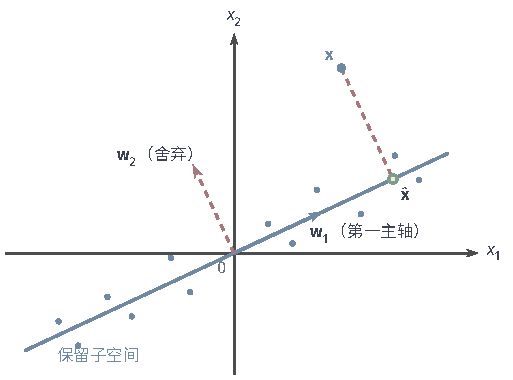
\includegraphics[width=86.935mm]{figures/04-classic-models/00-shared/tikz/dim-pca-projection/figure.pdf}
  \caption{二维到一维的正交投影示意。蓝色实线方向$\bm{w}_1$是保留的第一主轴，红色虚线方向$\bm{w}_2$是被舍弃的正交主轴。点$\bm{x}$投到$\widehat{\bm{x}}$，重构残差沿$\bm{w}_2$方向。图中散点为示意位置，未表示真实实验。}
  \label{fig:dim-pca-projection}
\end{figure}

\subsubsection{参数学习}
\label{sec:dim-pca-learning}

最优方向可以通过协方差的谱求出。在单位方向的约束目标中引入乘子$\lambda$，驻点方程为$\bm{S}\bm{w}=\lambda\bm{w}$，投影方差正好等于$\lambda$。按$\lambda_1\geq\cdots\geq\lambda_d\geq0$排序，前$k$个特征向量组成$\bm{V}_k$，其列称为\term{主成分方向}（principal component directions）。取$\bm{W}=\bm{V}_k$得到一个解析最优解；得分$\bm{X}\bm{V}_k$的经验协方差为$\operatorname{diag}(\lambda_1,\ldots,\lambda_k)$，所以这些得分不相关，统计独立还需要额外条件。

方向的唯一性需要分别看基矩阵、子空间与投影算子。一般最优$\bm{W}$是一组正交基，$\operatorname{span}(\bm{W})$是其张成的主子空间，$\bm{P}=\bm{W}\bm{W}^{\top}$是相应投影。若$\lambda_k>\lambda_{k+1}$，主子空间与投影唯一；子空间内部仍可以旋转，任意$k$阶正交矩阵$\bm{Q}$都使$\bm{W}\bm{Q}$给出同一投影，所有最优基可写成$\bm{V}_k\bm{Q}$。

坐标基的旋转却会改变各列及得分之间的关系。从$\bm{W}=\bm{V}_k$出发，若$\bm{Q}$混合不同特征值的方向，$\bm{W}\bm{Q}$的列一般不再是$\bm{S}$的特征向量，得分协方差$\bm{Q}^{\top}\operatorname{diag}(\lambda_1,\ldots,\lambda_k)\bm{Q}$一般也不再对角。因此，互不相关的主成分得分对应排序特征向量基$\bm{V}_k$，而非主子空间中的任意正交基。

如果进一步要求各列为排序后的特征向量，单特征值方向只差符号；所选范围内的重特征值允许在其重特征子空间中旋转。若$\lambda_k=\lambda_{k+1}$，重特征值跨过截断位置，最优主子空间和投影算子也可能不唯一。

实际计算通常对中心化数据作\term{奇异值分解}（singular value decomposition, SVD），写成$\bm{X}=\bm{U}\bm{\Sigma}\bm{V}^{\top}$。右奇异向量给出主方向，$\lambda_j=\sigma_j^2/n$，得分为$\bm{U}_k\bm{\Sigma}_k$。直接SVD无需显式形成$\bm{X}^{\top}\bm{X}$，可以避免条件数平方带来的数值困难。完整稠密分解约需$O(nd\min(n,d))$次运算，只求少数方向时还可使用截断算法；不同实现需要不同的矩阵和计算预算。

用同一批点比较不同方向，可以直接看出重构目标怎样选择主轴。图\ref{fig:dim-pca-objective}中，水平方向留下的平均平方残差为$0.8125$；改用SVD算出的第一主方向后，残差降为$0.25$。两图的样本、中心和坐标尺度都相同，变化只来自所保留的方向。

\begin{figure*}[tbp]
  \centering
  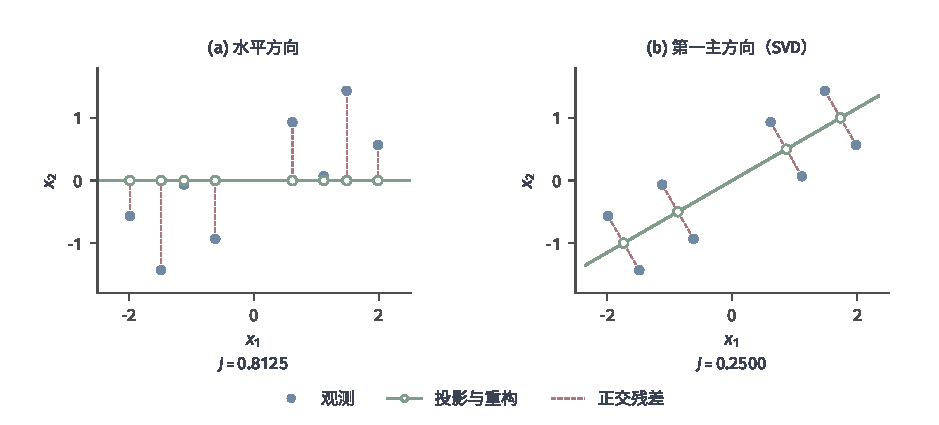
\includegraphics[width=159.000mm]{figures/04-classic-models/00-shared/matplotlib/dim-pca-objective/figure.pdf}
  \caption{PCA重构目标的数值对照。取八个无量纲点$(t,u)$，其中$t\in\{-2,-1,1,2\}$、$u\in\{-1/2,1/2\}$，统一逆时针旋转$30^\circ$；样本均值为零。蓝点为观测，绿线为保留方向，空心点为正交重构，红色虚线为残差；右图部分重构点重合。平均平方残差记为$J$，两个方向分别给出$0.8125$和$0.25$。第一主方向由这组数据的SVD实际计算，图中未人为指定拟合结果。}
  \label{fig:dim-pca-objective}
\end{figure*}

当$d\gg n$时，样本空间中的$n\times n$ Gram矩阵$\bm{X}\bm{X}^{\top}$更小。若$\bm{X}\bm{X}^{\top}\bm{u}_j=\sigma_j^2\bm{u}_j$且$\sigma_j>0$，右奇异向量可由$\bm{v}_j=\bm{X}^{\top}\bm{u}_j/\sigma_j$恢复。这仍是同一SVD；第\ref{sec:dim-kpca}节将沿样本空间计算引出核方法。

求出特征值后，可以衡量前$k$个方向保留的方差比例。\term{累计解释方差}（cumulative explained variance）定义为
\begin{equation}
  \eta_k=\frac{\sum_{j=1}^{k}\lambda_j}
                    {\sum_{j=1}^{d}\lambda_j}.
  \label{eq:dim-explained-variance}
\end{equation}
总方差非零时，可以按预先选择的比例确定$k$，也可以查看特征值随序号下降的碎石图。$85\%$、$95\%$等比例是经验阈值，并非预测信息的保证：低方差方向可能包含第\ref{sec:classification-lda-model}节的类别判别信息，高方差也可能来自量纲或背景干扰。是否标准化由特征单位和任务决定；服务于预测的维数选择应使用训练集内部的验证结果。

矩阵规模过大时，还可以近似求主子空间。随机化SVD先估计列空间，再分解较小的矩阵；增量PCA按批次更新子空间。二者以近似误差或特定更新规则换取内存与时间收益，评价时需要同时检查求解精度\scite{halko2011}

\subsubsection{理论分析}
\label{sec:dim-pca-theory}

\paragraph{表达能力}
PCA能否完整保留观测，取决于数据是否落在一个$k$维仿射子空间中。设观测$\bm X$有有限二阶矩，均值为$\bm\mu$、协方差为$\bm\Sigma_\star$，后者的有序特征值为$\lambda_1^\star\geq\cdots\geq\lambda_d^\star\geq0$。对任一秩$k$正交投影$\bm P$，重构残差的期望平方为$\operatorname{tr}((\bm I-\bm P)\bm\Sigma_\star)$。沿协方差特征方向分解这一量，保留最大的$k$项便得到
\begin{equation}
 \min_{\bm P}\mathbb E\lVert
   (\bm I-\bm P)(\bm X-\bm\mu)\rVert_2^2
   =\sum_{j>k}\lambda_j^\star.
 \label{eq:dim-pca-representation-error}
\end{equation}
右侧为零，恰好意味着观测以概率一落在所保留的仿射子空间中。数据只集中在子空间附近时，舍弃方差之和就是这一候选族无法消除的重构误差，增加求解精度不会减小它。

内在维数小并不足以使这个误差为零。例如在单位圆周上均匀取点，分布只沿一条曲线变化，协方差却为$\bm I_2/2$；任何一维PCA的期望重构误差都是$1/2$。若低秩信号再叠加独立、均值为零、协方差为$\tau^2\bm I_d$的观测噪声，任何秩$k$投影的残差中又至少包含$(d-k)\tau^2$的噪声方差。这里评价的是重构观测；恢复无噪声信号需要另换评价对象。低方差方向也可能承载类别信息，因此较小的重构误差本身不保证保留预测所需的信息。

\paragraph{收敛性}

固定数据上的最优重构可以由Eckart--Young低秩逼近定理说明\scite{eckart1936}下面将这一结果用于PCA的正交重构，再把它与估计总体子空间的问题分开。

在正交投影与平方误差设定下，前$k$维主子空间达到经验全局最优，最小误差等于舍弃特征值的总和。截断处的谱隙进一步决定投影是否唯一：

\begin{theorem}[PCA最优重构解的存在性与谱间隔下的唯一性]
  \label{thm:dim-pca-optimal}
  设$\bm{X}$已中心化，$1\leq k<d$，$\lambda_j$为$\bm{S}=\bm{X}^{\top}\bm{X}/n$按降序排列的特征值。则
  \[
    \min_{\bm{W}^{\top}\bm{W}=\bm{I}_k}
       \frac1n\lVert\bm{X}-\bm{X}\bm{W}\bm{W}^{\top}\rVert_F^2
       =\sum_{j=k+1}^{d}\lambda_j.
  \]
  前$k$个特征向量张成的子空间达到最小值。若$\lambda_k>\lambda_{k+1}$，最优投影算子$\bm{W}\bm{W}^{\top}$唯一，但子空间内的正交基不唯一。
\end{theorem}

\begin{proof}
在所有秩至多为$k$的矩阵中，截断SVD使平方Frobenius误差最小（参见\BookTheoremRef{thm:matrix-analysis-best-low-rank}{卷1《数学准备：计算、分析与几何》第5章“线性空间”第5.5.4节“秩约束下的矩阵逼近”}）。
截断SVD给出$\bm X\bm V_k\bm V_k^\top$，其平方误差为$\sum_{j>k}\sigma_j^2$；
除以$n$并代入$\lambda_j=\sigma_j^2/n$即得结论。
截断处的严格谱隙使主子空间与投影唯一，唯一的投影仍允许在其子空间中选择不同的正交基。
\end{proof}

迭代谱算法要逼近的是定理中的全局最优投影，可以用特征方程残差和方向正交误差检查数值精度。增加迭代可以改善求解误差；样本是否足以估计总体结构，则是下面的统计问题。

\paragraph{泛化性}
训练重构最优的子空间，仍可能在新样本上丢失更多变化。沿用期望风险记号，设$D_n$独立同分布于$P$，总体均值为$\bm\mu$、协方差为$\bm\Sigma_\star$。训练所得均值与投影为$\bar{\bm X}$、$\widehat{\bm P}$，新点的重构规则固定为
$\widehat r_n(\bm x)=\bar{\bm X}+\widehat{\bm P}(\bm x-\bar{\bm X})$。
其风险$R_n=\mathbb E_{\bm X\sim P}\lVert\bm X-\widehat r_n(\bm X)\rVert_2^2$中的新点独立于训练集。下面直接比较这一风险与最佳$k$维仿射重构，而不要求主方向估计唯一。

\begin{theorem}[PCA在有界观测下的期望重构风险界]
 \label{thm:dim-pca-risk}
 假设$\lVert\bm X-\bm\mu\rVert_2\leq r$几乎处处，$\bm S$是以样本均值中心化、分母为$n$的样本协方差。设$\widehat{\bm P}$为秩$k$正交投影，满足
 \[
 \operatorname{tr}(\bm S\widehat{\bm P})
 \geq\max_{\bm P\text{为秩}k\text{正交投影}}
       \operatorname{tr}(\bm S\bm P)-e_n,
 \qquad e_n\geq0.
 \]
 记$R_k^\star=\min_{\bm P}\operatorname{tr}((\bm I-\bm P)\bm\Sigma_\star)$。则
 \begin{equation}
  \mathbb E_{D_n}R_n
  \leq R_k^\star+\frac{2\sqrt{k}\,r^2}{\sqrt n}
          +\frac{(2\sqrt{k}+1)r^2}{n}
          +\mathbb E_{D_n}e_n.
  \label{eq:dim-pca-risk-bound}
 \end{equation}
\end{theorem}
\begin{proof}
将$\bm X-\bar{\bm X}$分成$\bm X-\bm\mu$与均值误差，独立新点的交叉项期望为零，得到
\[
 R_n=\operatorname{tr}((\bm I-\widehat{\bm P})\bm\Sigma_\star)
       +\lVert(\bm I-\widehat{\bm P})(\bar{\bm X}-\bm\mu)\rVert_2^2.
\]
设$\bm P_\star$为总体最优投影。在投影风险差中加入样本协方差，并使用经验最优性，有
\begin{equation}
 \begin{aligned}
 \operatorname{tr}((\bm P_\star-\widehat{\bm P})\bm\Sigma_\star)
 &\leq\operatorname{tr}((\bm P_\star-\widehat{\bm P})
                          (\bm\Sigma_\star-\bm S))+e_n\\
 &\leq2\sqrt{k}\,\lVert\bm S-\bm\Sigma_\star\rVert_F+e_n.
 \end{aligned}
 \label{eq:dim-pca-excess-risk}
\end{equation}
最后一步使用两个秩$k$投影的Frobenius范数至多各为$\sqrt k$。
令$\bm Y_i=\bm X_i-\bm\mu$及$\bm e=\bar{\bm X}-\bm\mu$，则
$\bm S=n^{-1}\sum_i\bm Y_i\bm Y_i^\top-\bm e\bm e^\top$。
独立性与$\lVert\bm Y_i\rVert_2\leq r$给出
\[
 \mathbb E\left\lVert\frac1n\sum_i\bm Y_i\bm Y_i^\top
                        -\bm\Sigma_\star\right\rVert_F
 \leq\frac{r^2}{\sqrt n},
 \qquad \mathbb E\lVert\bm e\rVert_2^2\leq\frac{r^2}{n}.
\]
因此$\mathbb E\lVert\bm S-\bm\Sigma_\star\rVert_F
\leq r^2/\sqrt n+r^2/n$。代入风险分解，并以$\lVert\bm e\rVert_2^2$控制均值项，得到结论。
\end{proof}

定理把总体重构拆成最佳线性近似误差、协方差与均值的估计误差，以及数值求解误差。精确谱分解使$e_n=0$；随机化SVD与增量近似应保留该项。风险界不需要谱隙，相近特征值对应的方向可以明显旋转，重构损失却只改变很少。若要估计方向本身，谱隙才成为另一项条件。

有界观测是本定理的明确条件，重尾或维数随样本量增长时需采用相应矩条件和估计方法。尖峰协方差模型与Marchenko--Pastur型谱极限说明样本谱可能偏离总体结构\scite{nadler2008,marchenko1967}这些参数或谱结论不能代替式\eqref{eq:dim-pca-risk-bound}所评价的新样本重构。奇异值阈值也应在指定噪声与损失条件下使用\scite{donoho2014threshold}

\subsubsection{优化泛化能力}

\paragraph{分离稀疏异常污染}
\label{sec:dim-robust-pca}

普通PCA以平方误差衡量重构，一小部分幅度很大的污染就可能拉动主方向。考虑固定摄像机拍摄的构造场景：背景基本不变，移动物体每帧只覆盖少量像素。把各帧排成观测矩阵$\bm{M}\in\mathbb{R}^{n\times d}$后，相似的背景可以用低秩矩阵$\bm{L}$表示，少量变化像素则放入稀疏矩阵$\bm{E}$。分别估计这两部分，可以让大幅度的局部变化留在扰动中，而不迫使背景子空间追随它们。这里的\term{鲁棒PCA}（robust PCA, RPCA）专指低秩加稀疏分解，稳健子空间估计还包括其他污染设定。

同时寻找低秩部分和稀疏部分时，直接最小化$\operatorname{rank}(\bm{L})+\lambda\lVert\bm{E}\rVert_0$存在组合困难。\term{主成分追踪}（principal component pursuit, PCP）用两个凸惩罚替代秩和非零元素数：
\begin{equation}
  \min_{\bm{L},\bm{E}}\
     \lVert\bm{L}\rVert_*+\lambda\lVert\bm{E}\rVert_1,
  \qquad \bm{M}=\bm{L}+\bm{E}.
  \label{eq:dim-pcp}
\end{equation}
核范数$\lVert\bm{L}\rVert_*=\sum_j\sigma_j(\bm{L})$鼓励较少的非零奇异值；$\lVert\bm{E}\rVert_1$为所有元素绝对值之和，鼓励较少的非零污染项。两个惩罚分别作用于整体秩结构与逐元素扰动。

\paragraph{表达能力}
低秩加稀疏模型可以精确表示“共享背景加少量任意幅度的像素污染”，前提是无污染矩阵确实低秩、污染确实只占少数位置。它不要求污染幅度小，却要求两部分能由结构区分。以$\bm e_i,\bm e_j$表示行、列空间中的坐标向量，取$\bm T=\bm e_i\bm e_j^\top$，它既是秩一矩阵，又只有一个非零元素；观测$\bm M=\bm T$既能解释为$(\bm L,\bm E)=(\bm T,\bm0)$，也能解释为$(\bm0,\bm T)$。只写低秩和稀疏，便无法判断哪一种是真实背景。

若还有稠密测量噪声，等式$\bm M=\bm L+\bm E$便不能同时把它解释成干净低秩信号与稀疏污染，需要允许剩余误差。整行损坏也不同于少量像素损坏，应按污染对象改用相应约束。

\paragraph{参数学习}
两个惩罚可以由\term{交替方向乘子法}（alternating direction method of multipliers, ADMM）分开求解，再通过重构约束协调。取惩罚参数$\rho>0$，引入与$\bm{M}$同形的$\bm{U}$作为缩放对偶变量，即拉格朗日乘子除以$\rho$。固定$\bm{U}$并略去无关常数，增广目标为
\[
  \lVert\bm{L}\rVert_*+\lambda\lVert\bm{E}\rVert_1
  +\frac{\rho}{2}
   \lVert\bm{M}-\bm{L}-\bm{E}+\bm{U}\rVert_F^2.
\]
固定$\bm{E}$更新$\bm{L}$，再用新$\bm{L}$更新$\bm{E}$，分别对应两种阈值运算。随后将尚未满足的重构误差加到$\bm{U}$，让下一轮继续校正约束偏差。从$\bm{U}^{(0)}=\bm{0}$开始时，一轮更新为
\begin{equation}
  \begin{aligned}
  \bm{L}^{(t+1)}&=\operatorname{SVT}_{1/\rho}
                  (\bm{M}-\bm{E}^{(t)}+\bm{U}^{(t)}),\\
  \bm{E}^{(t+1)}&=\mathcal{S}_{\lambda/\rho}
                  (\bm{M}-\bm{L}^{(t+1)}+\bm{U}^{(t)}),\\
  \bm{U}^{(t+1)}&=\bm{U}^{(t)}
                   +\bm{M}-\bm{L}^{(t+1)}-\bm{E}^{(t+1)}.
  \end{aligned}
  \label{eq:dim-rpca-admm}
\end{equation}
逐元素软阈值为$\mathcal{S}_{a}(u)=\operatorname{sign}(u)(|u|-a)_+$，$\operatorname{SVT}_{a}$则将同一运算作用于奇异值。模型中的$\bm{E}$代表稀疏扰动，迭代中的$\bm{U}$累积重构约束误差。为检查固定$\rho$下的停止条件，需要同时计算
\[
  \begin{aligned}
    r_{\mathrm{pri}}^{(t+1)}
      &=\lVert\bm{M}-\bm{L}^{(t+1)}-\bm{E}^{(t+1)}\rVert_F,\\
    r_{\mathrm{dual}}^{(t+1)}
      &=\rho\lVert\bm{E}^{(t+1)}-\bm{E}^{(t)}\rVert_F.
  \end{aligned}
\]
原始残差检查重构等式，对偶残差检查第二个子问题的变化是否仍破坏前一个子问题的平衡。两项均应低于按数据尺度设置的容差；迭代次数只是预算，不能代替这两项检查。

\paragraph{恢复与矩阵风险}
Candès等的精确恢复定理用不相干条件排除低秩信号集中在少数坐标的情形，并限制秩、污染比例与随机支持。满足后面定理\ref{thm:dim-rpca-matrix-risk}的条件时，PCP能恢复两部分，而不只是找到一个满足重构等式的分解\scite{candes2011rpca}。

\begin{theorem}[随机污染支持下的PCP恢复与矩阵风险]
 \label{thm:dim-rpca-matrix-risk}
 设$\bm M=\bm L_0+\bm E_0\in\mathbb R^{n\times d}$，
 $n_{\max}=\max(n,d)\geq2$、$n_{\min}=\min(n,d)$。
 固定秩$r_L$的$\bm L_0=\bm U\bm\Lambda\bm V^\top$，其奇异向量满足
 \[
 \begin{gathered}
 \max_i\lVert\bm U^\top\bm e_i\rVert_2^2\leq\mu r_L/n,
 \qquad
 \max_j\lVert\bm V^\top\bm e_j\rVert_2^2\leq\mu r_L/d,\\
 \lVert\bm U\bm V^\top\rVert_\infty\leq\sqrt{\mu r_L/(nd)}.
 \end{gathered}
 \]
 $\bm e_i$为相应空间的坐标向量，矩阵无穷范数在此为元素绝对值的最大值。
 污染符号与幅度固定，支持$\Omega$在所有含$s$个位置的子集中均匀抽取。
 存在绝对正常数$\rho_r,\rho_s,c$，使当
 \[
 r_L\leq\rho_r n_{\min}/[\mu(\log n_{\max})^2],
 \qquad s\leq\rho_s nd
 \]
 时，式\eqref{eq:dim-pcp}取$\lambda=1/\sqrt{n_{\max}}$，其全局解以至少$1-c n_{\max}^{-10}$的概率精确恢复$\bm L_0,\bm E_0$。
 若还知$|L_{0,ij}|\leq B$，将恢复矩阵逐元素截到$[-B,B]$得到$\widetilde{\bm L}$，则
 \begin{equation}
  \mathbb E_\Omega\frac{\lVert\widetilde{\bm L}-\bm L_0\rVert_F^2}{nd}
  \leq4B^2c n_{\max}^{-10}.
  \label{eq:dim-rpca-matrix-risk}
 \end{equation}
\end{theorem}
精确恢复的概率结论来自Cand\`es等的PCP定理\scite{candes2011rpca}。风险式在成功事件上为零，失败事件上每个元素的平方误差至多为$4B^2$，所以直接乘以失败概率即可。这里的随机性是当前矩阵中的污染支持，结论评价整矩阵恢复；PCP未学习一个处理独立新帧的共享编码器，不能将这个风险改称新帧重构风险。有限轮ADMM的求解误差也未包含在精确全局解结论中。

\paragraph{支持稠密测量噪声}
少量像素污染之外，每个像素还可能都有幅度较小的测量误差。这时精确等式会迫使低秩信号或稀疏污染吸收这部分误差。稳定PCP改为允许$\lVert\bm{M}-\bm{L}-\bm{E}\rVert_F\leq\delta$，用$\delta$限制剩余稠密误差的总量。它放松了重构约束，前面的无噪声精确恢复结论不能直接沿用。

\paragraph{支持成组的异常污染}
若整帧损坏，异常会占据观测矩阵的一整行，逐元素稀疏便不再准确描述污染方式。可以对污染矩阵按行施加组稀疏约束，让整条记录共同进入异常部分。视频背景、遮挡和传感器异常应据此区分局部像素污染与整条记录污染；约束改变后，两部分可识别的条件也需要重新检查。

\paragraph{利用已知子空间方向}
若已经知道部分背景方向，完全从观测重新寻找子空间会舍弃这项信息。侧信息变体把已知子空间特征写入分解的约束或表示，帮助限定仍需估计的信号方向\scite{dimChiang2016side}。收益取决于侧信息是否准确；错误方向也可能限制本来需要的信号，因而应连同其来源和误差一起检查。

\subsubsection{优化解释能力}

\label{sec:dim-sparse-pca}

普通PCA会综合全部坐标，即使只提取一个成分，也可能需要读取几乎所有变量。以基因表达分析为例，一个成分若由数千个基因以很小的权重共同组成，就不容易看出哪一小组基因解释了这项变化。\term{稀疏PCA}（sparse PCA）限制载荷中的非零项，把少量变量的要求与重构目标一同求解。它可能牺牲部分解释方差，换取更容易辨认和测量的变量组合；在普通PCA求解后直接删掉小载荷，通常不能得到这一受约束问题的最优解。Zou、Hastie与Tibshirani在2006年用回归式矩阵分解把成分提取与变量选择结合，并讨论基因表达等高维数据\scite{zou2006spca}其目标写为
\begin{equation}
  \begin{aligned}
  \min_{\bm{A},\bm{B}}\quad&
    \lVert\bm{X}-\bm{X}\bm{B}\bm{A}^{\top}\rVert_F^2
    +\lambda_1\sum_{j=1}^{k}\lVert\bm{b}_j\rVert_1
    +\lambda_2\lVert\bm{B}\rVert_F^2,\\
  \text{约束}\quad&\bm{A}^{\top}\bm{A}=\bm{I}_k.
  \end{aligned}
  \label{eq:dim-sparse-pca}
\end{equation}
在此目标中，$\bm{A},\bm{B}\in\mathbb{R}^{d\times k}$，$\bm{b}_j$是$\bm{B}$第$j$列，$\lambda_1,\lambda_2\geq0$。$\bm{B}$给出编码载荷，$\bm{A}$给出重构方向；$\ell_1$惩罚促使载荷稀疏，平方惩罚缓解相关变量造成的数值不稳定。

\paragraph{表达能力}
这一定义约束的是编码载荷$\bm B$，重构方向$\bm A$仍可使用全部变量。精确重构要求$\bm A\bm B^\top\bm x=\bm x$在数据支持上成立，因此数据必须落在$\bm A$张成的至多$k$维空间中。若数据只在$k$个原坐标上变化，取$\bm A=\bm B$为这些坐标向量，就能以稀疏载荷精确重构。

稀疏载荷也能编码某些稠密方向。设$\bm x=t\bm v$、$\lVert\bm v\rVert_2=1$，且第$j$个分量$v_j\ne0$。以$\bm e_j$表示第$j$个坐标向量，取$\bm A=\bm v$、$\bm B=\bm e_j/v_j$，只读取第$j$个变量便恢复$t$，再用$\bm A$重构整条直线。若$v_j$很小，这种编码需要较大的载荷幅度，也会放大该变量中的测量误差。额外幅度限制可能排除这一表示。无论载荷是否稀疏，重构仍落在一个固定线性子空间，式\eqref{eq:dim-pca-representation-error}仍给出其平方重构误差的下限。

\paragraph{参数学习}
惩罚目标未必会选择前述精确表示，因而需要按实际目标求解。交替求解时，固定$\bm{A}$，可以将$\bm{X}$分到$\bm{A}$的列空间与正交补：
\[
  \lVert\bm{X}-\bm{X}\bm{B}\bm{A}^{\top}\rVert_F^2
  =\lVert\bm{X}\bm{A}-\bm{X}\bm{B}\rVert_F^2
   +\lVert\bm{X}(\bm{I}-\bm{A}\bm{A}^{\top})\rVert_F^2.
\]
第二项与$\bm{B}$无关，所以编码载荷可以按列求弹性网回归。转而固定$\bm{B}$，需要最大化$\operatorname{tr}(\bm{A}^{\top}\bm{X}^{\top}\bm{X}\bm{B})$，这是寻找最佳正交对齐的Procrustes问题，可由SVD求解。交替更新通常得到局部解，初始化与惩罚强度的敏感性需要检查。

稀疏载荷让变量组合更容易辨认，同时也改变了得分之间的关系。$\bm{B}$各列通常不正交，得分方差可能重叠，因此各成分方差之和不能直接作为标准PCA式的解释方差。基因表达和文本等应用需要同时评价稀疏程度、重构效果与跨样本稳定性。

\paragraph{泛化性}
稀疏PCA不能原样套用正交PCA的风险式，因为$\bm A\bm B^\top$一般不是正交投影。仍可复用协方差比较：已知总体零均值时，令$\bm Q=(\bm I-\bm A\bm B^\top)^\top(\bm I-\bm A\bm B^\top)$，总体重构误差就是$\operatorname{tr}(\bm Q\bm\Sigma_\star)$。若抽样前另规定$\lVert\bm B\rVert_F\leq b$，则$\lVert\bm Q\rVert_F\leq\sqrt d(1+b)^2$；再结合有界观测下$\mathbb E\lVert\bm S-\bm\Sigma_\star\rVert_F\leq r^2/\sqrt n$，便能按定理\ref{thm:dim-pca-risk}的两次偏差比较方式控制风险。式\eqref{eq:dim-sparse-pca}的惩罚须同时除以$n$，在经验与总体目标中保持相同。均值也由样本估计时，还需增加均值误差；这组条件不会由载荷稀疏自动成立。

\subsubsection{优化计算能力}

持续接收新帧时，静态PCP要处理不断增长的矩阵，历史观测的存储与反复分解会增加负担。在线变体改为随观测到达更新子空间及污染估计\scite{dimFeng2013orPca}。它们需要规定保留哪些历史信息、怎样允许子空间变化及何时更新，静态矩阵的恢复结论不能自动解释整个流式过程。

\subsubsection{支持响应监督的降维场景}

用于预测时，方差较大的方向未必含有响应信息。例如，传感器读数可能主要随环境温度变化，待预测的状态却只体现为一个变化较小的坐标。这时需要改变方向的评价目标，而不只是增加PCA的成分数。第\ref{sec:regression-regularization}节的PCR按输入方差选成分，可能先删掉这个坐标；PLS让响应参与构造方向，第\ref{sec:classification-lda-model}节的线性判别分析则比较类间变化与类内变化。它们与PCA共享线性表示形式，选择方向的目标却不同。

Li在1991年提出的切片逆回归沿另一条路线，观察不同响应范围下的输入均值怎样改变，即利用$\mathbb{E}[\bm{x}\mid y]$寻找有效方向\scite{li1991sir}。它不直接寻找输入方差最大的轴；相应线性与非退化条件决定哪些响应方向能由条件均值显示，对称响应可能使这些均值不变而遗漏有关方向。

监督降维组合特征形成新方向，特征选择保留原坐标子集，两者可以共同使用。响应参与后，表示学习也增加了监督拟合与选择的环节。比较预测收益时，应将方向学习、特征选择和预测器都放在训练折内，以相同下游任务比较无监督表示、监督表示和不降维基线。

\subsubsection{小结}
\label{sec:dim-pca-summary}

PCA用一组共享线性方向压缩输入，并按平方重构目标选择保留的变化。维数决定压缩程度，变量尺度决定不同测量怎样参与比较；大幅度异常记录也可能改变主要方向。保留较多方差适合重构，却不必保留预测所需的低方差信息。

变量解释与异常污染需要不同调整。稀疏PCA让编码只读取少量变量，换取更容易辨认的组合，同时改变求解与成分方差的计算。低秩加稀疏的RPCA则把局部污染与共享信号分开，代价是更强的结构区分条件和迭代矩阵计算。前者限制载荷，后者改变观测分解，不能相互替代。

若表示服务于有监督预测，方向选择还应对应响应信息，可比较PLS、判别投影或切片逆回归等目标。若需解释测量噪声及潜变量不确定性，第\ref{sec:dim-ppca}节的概率模型提供另一种假设。选择时应先确认需要解释的是变量、污染、预测关系还是观测生成，再评价相应代价。

\subsection{典型相关分析（CCA）}
\label{sec:dim-cca}

同一对象可以有两组测量，例如图像特征与对应文字特征。分别做PCA保留的是各侧最大的变化，却未必是两侧共有的内容。用一个构造例子看这一区别：设$S,U,V$是互相独立、均值为零且方差有限的实值随机变量，$S$表示共同变化，$U,V$表示各侧独有的变化。两组观测为$(S,U)$与$(S,V)$，并令$U,V$的方差都大于$S$。按总体协方差各取一个PCA主成分时，两侧会分别选到$U,V$，丢掉共同的$S$。\term{典型相关分析}（canonical correlation analysis, CCA）改为选择两侧得分相关系数最大的投影；当$S$的方差非零时，两侧选取$S$就得到总体相关系数1。Hotelling的经典工作建立了这一双视图分析框架\scite{hotelling1936cca}。

\subsubsection{模型结构}
\label{sec:dim-cca-structure}

将成对观测中心化，记$\bm{x}\in\mathbb{R}^{d_x}$、$\bm{y}\in\mathbb{R}^{d_y}$，两侧协方差为$\bm{\Sigma}_{xx}$、$\bm{\Sigma}_{yy}$，交叉协方差为$\bm{\Sigma}_{xy}=\mathbb{E}[\bm{x}\bm{y}^{\top}]$。用同一批配对样本估计这些矩阵后，第一对方向按投影相关系数选择：
\begin{equation}
  \max_{\bm{w}_x,\bm{w}_y}
  \frac{\bm{w}_x^{\top}\bm{\Sigma}_{xy}\bm{w}_y}
  {\sqrt{\bm{w}_x^{\top}\bm{\Sigma}_{xx}\bm{w}_x}
   \sqrt{\bm{w}_y^{\top}\bm{\Sigma}_{yy}\bm{w}_y}}.
  \label{eq:dim-cca-correlation}
\end{equation}
相关系数只有在两侧投影方差均非零时有定义。缩放方向不改变相关性，因此可以令两侧方差均为$1$，将求解转为最大化交叉协方差。

图\ref{fig:dim-cca-shared}用两个视图比较方差与共有信息。各自方差最大的坐标$u$、$v$相互独立，较小方差的坐标却同为$t$，所以PCA与CCA会选择不同方向。此比较保留原坐标的方差；逐坐标标准化改变方差结构，也会改变PCA选择。

\begin{figure*}[!ht]
  \centering
  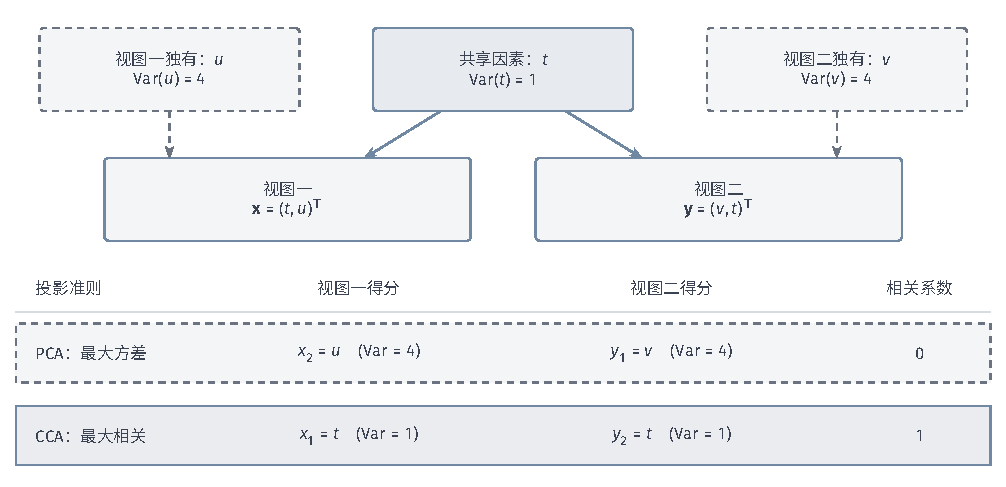
\includegraphics[width=169.000mm]{figures/04-classic-models/00-shared/tikz/dim-cca-shared/figure.pdf}
  \caption{CCA提取共有变化的构造例子。设$t,u,v$相互独立且均值为零，方差依次为$1,4,4$；两视图为$\bm{x}=(t,u)^\top$和$\bm{y}=(v,t)^\top$。实线连接共享因素，虚线连接各视图独有因素。各保留一维时，PCA选择$u,v$，CCA选择$t,t$，对应相关系数分别为$0$和$1$。箭头表示坐标构造关系，图中结论针对给定总体，不是样本拟合结果。}
  \label{fig:dim-cca-shared}
\end{figure*}

提取多对得分时，要求同一视图内$\bm{W}_x^{\top}\bm{\Sigma}_{xx}\bm{W}_x=\bm{I}_k$、$\bm{W}_y^{\top}\bm{\Sigma}_{yy}\bm{W}_y=\bm{I}_k$，使各得分方差为一且互不相关。这是协方差度量下的正交，原坐标中的方向未必欧氏正交。跨视图得分协方差可对角化为$\operatorname{diag}(\rho_1,\ldots,\rho_k)$，可识别的方向对数则同时受维数、样本秩与交叉协方差秩限制。

\subsubsection{参数学习}
\label{sec:dim-cca-learning}

两侧协方差正定时，可以先白化，使每侧协方差变成单位阵。白化后的交叉协方差及其SVD为
\[
  \bm{K}=\bm{\Sigma}_{xx}^{-1/2}
               \bm{\Sigma}_{xy}\bm{\Sigma}_{yy}^{-1/2},
  \qquad
  \bm{K}=\bm{U}\bm{D}\bm{V}^{\top}.
\]
令$\bm{a}=\bm{\Sigma}_{xx}^{1/2}\bm{w}_x$、$\bm{b}=\bm{\Sigma}_{yy}^{1/2}\bm{w}_y$，方差约束成为单位范数约束，目标成为$\max\bm{a}^{\top}\bm{K}\bm{b}$。取$\bm{K}$的首对左右奇异向量，就达到最大奇异值；多对方向由相应奇异向量依次取得：
\begin{equation}
  \bm{W}_x=\bm{\Sigma}_{xx}^{-1/2}\bm{U}_k,\qquad
  \bm{W}_y=\bm{\Sigma}_{yy}^{-1/2}\bm{V}_k,
  \label{eq:dim-cca-svd}
\end{equation}
$\bm{D}$的前$k$个对角元给出典型相关系数。实现白化时，可以使用Cholesky分解和三角求解，避免显式形成逆矩阵。

这一求解也可写成广义特征值问题。约束驻点满足$\bm{\Sigma}_{xy}\bm{w}_y=\rho\bm{\Sigma}_{xx}\bm{w}_x$及另一侧的对称方程，消去$\bm{w}_y$后得到
\[
  \bm{\Sigma}_{xy}\bm{\Sigma}_{yy}^{-1}
       \bm{\Sigma}_{yx}\bm{w}_x
  =\rho^2\bm{\Sigma}_{xx}\bm{w}_x.
\]


\subsubsection{理论分析}

\paragraph{表达能力}
CCA寻找的是两侧能用线性得分表达的共同变化。两侧协方差正定时，白化交叉协方差$\bm K=\bm\Sigma_{xx}^{-1/2}\bm\Sigma_{xy}\bm\Sigma_{yy}^{-1/2}$的奇异值$\rho_1\geq\rho_2\geq\cdots$就是可达的典型相关系数。对标准化得分$U,V$，有$\mathbb E(U-V)^2=2(1-\rho)$；因此$\rho=1$当且仅当两侧得分以概率一相同。前$k$对方向能保留$k$项最强的线性共有变化。各对标准化得分的均方差分别为$2(1-\rho_j)$，所以这一目标也直接给出了尚未匹配的共有变化。本节开头共享变量$S$的例子满足$\rho_1=1$，所以这一误差为零；各侧独有的$U,V$却无需保留。

线性得分可能完全看不到非线性依赖。例如$X\sim\mathcal N(0,1)$、$Y=X^2-1$时，$\mathbb E[XY]=0$，一维CCA的最大相关系数为零，但$Y$由$X$确定。把$X^2-1$纳入第一侧特征后才有可能匹配这一关系。这解释了核CCA扩展候选特征的作用；能否表达具体依赖仍取决于所选核，相关性目标也不保证恢复各视图的全部信息。


\paragraph{收敛性}
当两侧协方差正定时，白化把约束变为单位球面或正交列约束，可行集紧致，最大值存在。式\eqref{eq:dim-cca-svd}的SVD直接给出全局解；最大相关系数唯一，但对应方向只有在相应奇异值单一时才除符号外唯一。重奇异值允许在其子空间中旋转。协方差奇异时，应先限制到有正方差的支持空间；加入正则化则改变了原约束。迭代SVD的速度由具体求解器和奇异值间隔决定，CCA目标本身没有一个独立于谱间隔的统一迭代次数。

\paragraph{泛化性}
CCA的训练相关性可能很高，但新的一对观测不一定仍沿相同方向共同变化。可用总体标准化投影的均方差评价这一任务：对方向$\bm a,\bm b$，令
\[
 R(\bm a,\bm b)
 =\frac12\mathbb E\left(
 \frac{\bm a^\top\bm X}{\sqrt{\bm a^\top\bm\Sigma_{xx}\bm a}}
 -\frac{\bm b^\top\bm Y}{\sqrt{\bm b^\top\bm\Sigma_{yy}\bm b}}
 \right)^2
 =1-\rho(\bm a,\bm b).
\]
均值在此设为已知的零，$\rho$为式\eqref{eq:dim-cca-correlation}的总体相关系数。方向缩放不改变风险，所以可取两方向的欧氏范数为一。

\begin{theorem}[CCA在协方差非退化与扰动受控条件下的期望对齐风险界]
 \label{thm:dim-cca-risk}
 设$n$对观测独立同分布，已知总体均值为零，
 $\lVert(\bm X^\top,\bm Y^\top)^\top\rVert_2\leq r$几乎处处。
 记总维数为$q=d_x+d_y$，假设两侧总体协方差的最小特征值均至少为$v>0$。
 用已知零均值的经验二阶矩计算$\widehat\rho_n$，学习器的输出满足
 $\widehat\rho_n(\widehat{\bm a},\widehat{\bm b})
 \geq\sup_{\bm a,\bm b}\widehat\rho_n(\bm a,\bm b)-e_n$。
 对$0<\delta<1$，令
 \[
 \zeta_n=q r^2\sqrt{\frac{2\log(2q^2/\delta)}n}.
 \]
 若$\zeta_n\leq v/2$，则以至少$1-\delta$的训练抽样概率，
 \begin{equation}
 R(\widehat{\bm a},\widehat{\bm b})
 \leq\inf_{\bm a,\bm b}R(\bm a,\bm b)
       +\frac{8\zeta_n}{v}+e_n.
 \label{eq:dim-cca-risk}
 \end{equation}
\end{theorem}
\begin{proof}
对联合二阶矩的$q^2$个元素用Hoeffding界与并集界，得到全矩阵算子误差至多$\zeta_n$。两侧投影方差至少为$v$，经验方差至少为$v/2$。分子协方差的扰动不超过$\zeta_n$；将分母的两个方差逐项替换，并使用$|\rho|\leq1$，得到全体方向上的
$|\widehat\rho_n-\rho|\leq4\zeta_n/v$。
总体最优方向与经验选中方向各承担一次这一偏差，再加经验求解误差，即得结论。
\end{proof}

这里的风险是新配对观测的共有变化损失，概率界覆盖训练后选择的方向；它并未评价某一视图独有的信息。已知均值的设定省去了均值估计项，实际样本中心化需另外控制该项。协方差接近奇异时，分母使界变差，这也解释了小样本高维CCA的风险；加入正则项可以稳定分母，同时改变比较的风险。核CCA及深度CCA还需控制所选变换的复杂度，不能直接沿用固定线性方向的维数$q$。

\subsubsection{优化表达能力}

两侧共有的信息未必表现为线性相关。前面$Y=X^2-1$的例子中，只有把平方变化纳入候选特征，才可能匹配这一依赖。核CCA先固定两侧核映射，再在特征空间中匹配相关性；深度CCA则把两侧变换也纳入训练\scite{andrew2013dcca}。固定核预先规定哪些依赖可进入表示；联合学习变换使表示随数据调整，同时增加参数拟合与验证的成本。学习后的参数映射可用前向计算编码新样本，核形式则仍需按训练样本展开计算。

\subsubsection{优化泛化能力}

每侧变量数接近或超过配对样本数时，样本协方差可能奇异，前面的白化和求逆就不能按满秩形式执行。可以只在非零方差子空间中求解，或分别加$\lambda_x\bm{I}$、$\lambda_y\bm{I}$进行正则化。正则化改变了归一化度量，训练相关系数因而需要配合留出配对样本的相关性一起评价。

\subsubsection{小结}
\label{sec:dim-cca-summary}

CCA适合从配对观测中提取共有变化，相关性目标与单侧方差目标不同。某一视图独有却重要的信息可能不被保留，相关性也不能单独说明因果关系；使用前要判断两侧是否确实存在希望保留的共同内容。

样本少而维数高时，正则化稳定两侧方差的归一化，同时改变方向选择。共有关系非线性时，核CCA先规定特征映射，深度CCA再将两侧变换纳入训练。后一类方法增加表达与参数学习的自由度，也增加拟合成本；训练相关性应配合未用于拟合的配对观测检验，不能只用更大的训练值选择模型。

\subsection{独立成分分析（ICA）}
\label{sec:dim-ica}

两个麦克风同时录到两个人的声音，每条记录都是两个声源的不同比例混合。PCA可以找出变化较大、彼此不相关的方向，却没有理由让这些方向恰好对应两个说话人。协方差为零只排除了线性相关，例如$X\sim\mathcal{N}(0,1)$时，$X$与$X^2$的协方差为零，后者却完全由前者确定。\term{独立成分分析}（independent component analysis, ICA）进一步假设源信号独立，利用非高斯分布中的信息寻找解混方向，用于说话人分离、脑电活动分析和眼动伪迹分离等任务\scite{comon1994ica}这些假设决定能否识别声源；去相关本身并不能完成分离。

信息论提供了另一种减少分量依赖的准则。Bell与Sejnowski在1995年研究非线性网络中的信息传递，推导出利用协方差以外统计信息的学习规则，并讨论未知混合语音的分离和未知回声的消除\scite{bell1995infomax}这类问题称为盲信号处理，因为混合或传播过程未知；对源信号的结构仍需作出假设。

\subsubsection{模型结构}
\label{sec:dim-ica-structure}

为说明解混关系，先取中心化、无噪声且源数等于观测通道数的模型：
\begin{equation}
  \bm{x}=\bm{A}\bm{s},\qquad
  \bm{z}=\bm{W}^{\top}\bm{x},\qquad
  \bm{W}^{\top}=\bm{A}^{-1}.
  \label{eq:dim-ica-model}
\end{equation}
混合矩阵$\bm{A}\in\mathbb{R}^{d\times d}$可逆，源$\bm{s}$的分量相互独立。此处$\bm{W}$的列存放解混方向，所以$\bm{W}=\bm{A}^{-\top}$。若将$\bm{A}^{-1}$直接称为解混矩阵，则编码用它左乘观测；两种记法描述同一运算。

\subsubsection{参数学习}
\label{sec:dim-ica-learning}

存在密度时，可以比较解混分量的联合分布与边际乘积，用KL散度衡量剩余依赖。写成熵的形式为
\[
  I(z_1,\ldots,z_d)
  =\sum_{j=1}^{d}h(z_j)-h(\bm{z}),
\]
$h$为微分熵，上式要求各项有定义；散度为零恰好对应分量独立。也可以在单位方差约束下寻找非高斯方向，例如最大化负熵$J(z)=h(g)-h(z)$，其中$g$与$z$均值、方差相同且服从高斯分布。独立量相加趋向高斯提供了分离的直觉，具体对比量在有限线性组合中的性质仍需检验，不能直接由中心极限定理得到严格单调性。

指定各源密度$p_j$后，还可以按观测似然估计解混方向。变量替换同时改变密度和体积，得到
\begin{equation}
  \ell(\bm{W})
  =n\log|\det\bm{W}|
   +\sum_{i=1}^{n}\sum_{j=1}^{d}
        \log p_j(\bm{w}_j^{\top}\bm{x}_i).
  \label{eq:dim-ica-likelihood}
\end{equation}
行列式项是解混Jacobian对体积的校正。互信息、非高斯性与似然从不同角度利用分布信息；近似对比函数或错误源密度会改变目标，得到的方向也可能不同。

求独立方向之前，通常先去除协方差中的尺度和相关性。\term{白化}（whitening）将协方差变成单位阵：若$\bm{S}=\bm{V}\bm{\Lambda}\bm{V}^{\top}$且保留特征值为正，取$\widetilde{\bm{x}}=\bm{\Lambda}^{-1/2}\bm{V}^{\top}\bm{x}$。源方差规范为$1$后，白化空间中的混合矩阵正交，剩下的是方向选择。

图\ref{fig:dim-ica-whitening}给出白化仍未分离源的例子。左图协方差已为单位阵，但$x_1$接近边缘时，$x_2$允许的区间随之改变，两个分量仍依赖。旋转到右图源坐标后，均匀方形的联合分布才分成两个一维均匀分布。旋转前后的协方差相同，需要更完整的分布信息选择方向。

\begin{figure}[!ht]
  \centering
  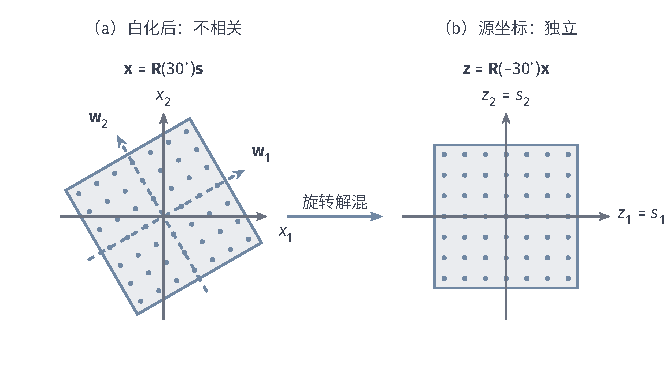
\includegraphics[width=112.000mm]{figures/04-classic-models/00-shared/tikz/dim-ica-whitening/figure.pdf}
  \caption{白化与独立源恢复的区别。设$s_1,s_2$独立且均服从$\mathcal{U}[-\sqrt3,\sqrt3]$，$\bm{R}(\theta)$为逆时针旋转矩阵。左图为$\bm{x}=\bm{R}(30^\circ)\bm{s}$，右图为逆旋转恢复的$\bm{s}$；两者协方差均为$\bm{I}_2$，只有右侧所示坐标对应独立源。实线轮廓为总体支持域，圆点为确定性格点，虚线箭头为解混方向。图为无量纲构造示意，未运行ICA优化；该方形解混本身不减少维数。}
  \label{fig:dim-ica-whitening}
\end{figure}

FastICA用光滑非二次函数$G$构造非高斯性对比量。单位方向$\bm{u}$在白化数据上产生方差为$1$的投影$\bm{u}^{\top}\widetilde{\bm{x}}$，可以将其与标准高斯变量$\nu$比较：
\begin{equation}
  J_G(\bm{u})
  =\left[
    \mathbb{E}G(\bm{u}^{\top}\widetilde{\bm{x}})
    -\mathbb{E}G(\nu)
  \right]^2,
  \qquad \lVert\bm{u}\rVert_2=1.
  \label{eq:dim-fastica-contrast}
\end{equation}
该目标近似前述负熵，其性质取决于$G$的选择。令$g=G'$；括号内的差非零、且期望与微分可交换时，$J_G$的球面驻点满足$\mathbb{E}G(\bm{u}^{\top}\widetilde{\bm{x}})$的约束驻点方程
\[
  \bm{a}(\bm{u})
  :=\mathbb{E}\!\left[\widetilde{\bm{x}}
       g(\bm{u}^{\top}\widetilde{\bm{x}})\right]
  =\beta\bm{u},
  \qquad
  \beta=\bm{u}^{\top}\bm{a}(\bm{u}).
\]
乘子$\beta$对应单位范数约束。近似求解时，在当前点固定$\beta$，并将Jacobian中的
$\mathbb{E}[\widetilde{\bm{x}}\widetilde{\bm{x}}^{\top}
g'(\bm{u}^{\top}\widetilde{\bm{x}})]$
近似为$c\bm{I}$，其中$c=\mathbb{E}g'(\bm{u}^{\top}\widetilde{\bm{x}})$。白化给出单位协方差，加上$g'$权重后的矩阵仍需这一步近似。若$c-\beta\ne0$，近似Newton步为
\[
  \bm{u}-\frac{\bm{a}(\bm{u})-\beta\bm{u}}{c-\beta}
  =\frac{c\bm{u}-\bm{a}(\bm{u})}{c-\beta}.
\]
方向可作符号翻转，归一化又消去非零标量，所以更新可直接使用$\bm{a}(\bm{u})-c\bm{u}$。将期望换成样本平均，从当前单位方向$\bm{u}^{(t)}$出发，就得到FastICA固定点更新：
\begin{equation}
  \begin{aligned}
  \bm{v}^{(t+1)}
    &=\frac1n\sum_{i=1}^{n}
      \widetilde{\bm{x}}_i
           g((\bm{u}^{(t)})^{\top}\widetilde{\bm{x}}_i)\\
    &\quad-\left[\frac1n\sum_{i=1}^{n}
      g'((\bm{u}^{(t)})^{\top}\widetilde{\bm{x}}_i)\right]\bm{u}^{(t)},\\
  \bm{u}^{(t+1)}
    &=\bm{v}^{(t+1)}/\lVert\bm{v}^{(t+1)}\rVert_2.
  \end{aligned}
  \label{eq:dim-fastica}
\end{equation}
常用$G(u)=\log\cosh u$或$G(u)=u^4/4$，对应$g(u)=\tanh u$和$g(u)=u^3$；后者的四次矩对极端值更敏感。多个成分可逐个与已求方向正交化，也可整组对称正交化。停止时检查方向变化，并把符号翻转计为同一方向\scite{hyvarinen1999fastica}

FastICA的收敛速度取决于源分布、对比函数与初始化，更新向量接近零时需重新初始化或调整设置。Infomax按输出非线性最大化输出熵，采用梯度更新；JADE通过联合对角化四阶累积量矩阵使用高阶统计信息。比较这些算法的成本，需要同时计入每次更新所用的信息与运算。

\subsubsection{理论分析}

\paragraph{表达能力}
在式\eqref{eq:dim-ica-model}的无噪声可逆线性混合中，候选解混矩阵包含$\bm A^{-1}$，所以存在精确恢复全部源的表示。若独立源非退化且至多一个为高斯，观测分布还可把这些源识别到排列与非零缩放的等价范围内\scite{comon1994ica}。其关键是：两个独立的源表示若由可逆线性变换相连，独立性限制了同一个非高斯源不能任意混入不同输出；高斯子空间则允许保持独立性的正交旋转。于是交换源及混合列，或作反向缩放，仍无法由观测区分，但除此之外的任意旋转通常会破坏独立性。

两个或更多标准高斯源组成的子空间可任意正交旋转而保持相同联合分布，因而不能恢复其中每个物理源的方向。混合矩阵秩亏时，不存在定义在整个源空间上的线性逆；若源支持包含仅沿其零空间相差的两种状态，它们产生相同观测，任何解混规则都无法区分。若观测还含一般的加性测量噪声，即使使用真实$\bm A^{-1}$，输出也为$\bm s+\bm A^{-1}\bm\epsilon$；无噪声的精确恢复结论不能消去这一项。源本身相关或混合关系非线性时，也未必存在使所有输出独立的线性变换。方形ICA保留全部通道数，若再压缩到更少坐标，还需要说明舍弃哪些源。



\paragraph{收敛性}
对白化后有限样本，若对比函数连续，单位方向或正交矩阵的可行集紧致，对比目标的最大值便存在；这不保证源成分可识别，也不保证极值唯一。FastICA是固定点更新，未必逐步改善同一目标，归一化向量为零时甚至没有下一步。若更新映射在某个固定点邻域内有定义、映射该邻域到自身，且导数算子范数至多为$q<1$，则从该邻域出发有$\lVert\bm u^{(t)}-\bm u_\star\rVert_2\leq q^t\lVert\bm u^{(0)}-\bm u_\star\rVert_2$；方向符号按一致方式选取。这是局部收缩条件给出的速度，实际$q$依赖分布、对比函数和初始化，不能推广为任意数据上的全局保证。

\paragraph{泛化性}
FastICA把总体期望换成样本平均，所需保证是训练选出的非高斯方向在新观测上仍有相近的对比值。

\begin{theorem}[FastICA在固定白化与有界输入下的期望对比风险界]
 \label{thm:dim-ica-risk}
先考虑一个方向，并在训练前固定白化变换。设白化观测$\widetilde{\bm X}$独立同分布且$\lVert\widetilde{\bm X}\rVert_2\leq r$，令
$h(t)=G(t)-\mathbb E G(\nu)$。
假设在$[-r,r]$上$|h(t)|\leq B$且$h$为$L$-Lipschitz。用两个独立新观测定义
\[
 R_G(\bm u)=\mathbb E\bigl[B^2
       -h(\bm u^\top\widetilde{\bm X})
        h(\bm u^\top\widetilde{\bm X}')\bigr]
       =B^2-J_G(\bm u),\qquad\lVert\bm u\rVert_2=1.
\]
这一非负损失把最大化非高斯性写成明确的期望风险；样本版本是样本均值的平方，而非假定$n^2$个点对相互独立。

记$\widehat J_{G,n}$为式\eqref{eq:dim-fastica-contrast}的经验版本，学习器输出满足
\[
 \widehat J_{G,n}(\widehat{\bm u})
 \geq\sup_{\lVert\bm u\rVert_2=1}\widehat J_{G,n}(\bm u)-e_n.
\]
单位方向的$\epsilon$覆盖数至多为$(1+2/\epsilon)^d$。对覆盖点的样本均值作集中，再用Lipschitz性扩展到全部方向，取$\epsilon=1/n$可得
\begin{equation}
 \begin{aligned}
 \mathbb E_{D_n}R_G(\widehat{\bm u})
 &\leq\inf_{\lVert\bm u\rVert_2=1}R_G(\bm u)
       +\frac{8BLr}{n}\\
 &\quad+4B^2\sqrt{\frac{2[d\log(1+2n)+\log2]}n}
       +\mathbb E_{D_n}e_n.
 \end{aligned}
 \label{eq:dim-ica-risk}
\end{equation}
\end{theorem}

具体地，所有方向上均值的期望偏差至多为
\[
 2Lr/n+B\sqrt{2[d\log(1+2n)+\log2]/n}.
\]
两个均值都在$[-B,B]$内，故平方差至多为均值差的$2B$倍，再按经验最优性承担两次偏差，得到该式。高概率版本将$\log2$换成$\log(2/\delta)$。

这一结论控制所选$G$的期望对比风险，FastICA的局部求解保留在$e_n$中。源是否真正分离还需对比函数在指定源模型下识别真实方向，并控制风险差到方向误差的关系。错误源模型或对比函数可以有很低的对比风险，却不能恢复声源。同一批数据上估计白化矩阵也增加统计误差，不能当作定理中的固定预处理。

\subsubsection{小结}
\label{sec:dim-ica-summary}

ICA从去相关转向独立源识别，依赖源独立、非高斯与可识别性条件。标准方形ICA仍输出原维数；先截断白化空间，或取源数少于通道数的模型，才同时压缩。源数多于通道数时是欠定混合，通常需要稀疏等额外结构；非线性混合、相关源、多个高斯源及强噪声也需要不同的识别条件与算法。

\subsection{非负矩阵分解（NMF）}
\label{sec:dim-nmf}

在词频、光谱强度或像素亮度的表示中，观测量本身非负。如果希望把一条记录解释为几类成分的叠加，普通线性分解中的负基与负系数就不容易对应“加入了多少某种成分”。\term{非负矩阵分解}（nonnegative matrix factorization, NMF）同时要求基与系数非负，使每个成分只增加重构值。例如，文本可由几个非负的词频模式相加表示，一张图像可由若干非负部件叠加表示。非负约束表达了这种加性解释，但学得的成分是否对应有意义的主题或部件，仍需结合数据检查。

% 为两条完整的历史文献边注保留空间。
\Needspace{12\baselineskip}
非负结构可以与不同的误差模型配合。Paatero与Tapper在1994年根据环境测量误差加权残差，并在正矩阵分解中施加非负约束\scite{paatero1994nmf}Lee与Seung在1999年用人脸和文本说明加性表示如何形成组成成分\scite{lee1999nmf}两项工作分别强调测量约束与部件表示，损失及应用假设也随所解释的对象而变。

\subsubsection{模型结构}
\label{sec:dim-nmf-structure}

将非负观测排成$\bm{X}\in\mathbb{R}_{+}^{n\times d}$，寻找较少的共享基及各样本的非负系数：
\begin{equation}
  \bm{X}\approx\bm{W}\bm{H},\qquad
  \bm{W}\in\mathbb{R}_{+}^{n\times k},\quad
  \bm{H}\in\mathbb{R}_{+}^{k\times d}.
  \label{eq:dim-nmf-factorization}
\end{equation}
此处$\bm{W}$存放样本系数，与PCA的正交基约定不同；第$i$行是样本$i$的表示，$\bm{H}$各行是共享基。文档可由主题词模式相加，光谱可由成分谱相加。非负约束规定这种加性关系，基是否局部化、系数是否稀疏以及主题是否可读，则需要数据与额外约束支持。

图\ref{fig:dim-nmf-parts}用固定的横条与竖条基演示加性重构。九个像素按行展开后，$\bm{H}$的两行为基的转置，系数$(0.6,1.0)$给出右侧图案。中心像素同时获得两项贡献，值为$1.6$。这一固定字典下，两系数足以描述该图案；压缩成本还需计入字典，一般观测也可能存在重构误差。

\begin{figure}[htbp]
  \centering
  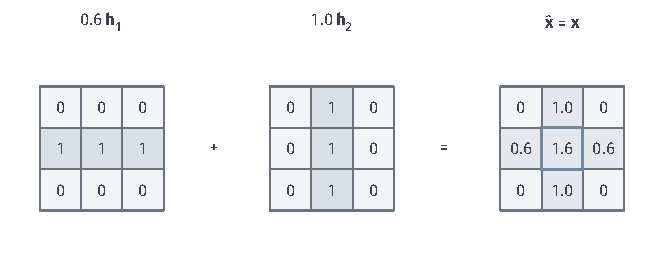
\includegraphics[width=112.000mm]{figures/04-classic-models/00-shared/tikz/dim-nmf-parts/figure.pdf}
  \caption{两个非负基的加性重构。左侧两幅$3\times3$栅格分别给出未加权的横条、竖条基，外侧系数为$0.6$与$1.0$；右侧为逐像素加权和，粗框中心格等于$0.6+1.0=1.6$。数值无量纲，本构造恰好精确重构，不表示NMF总能学出这样的部件或保证唯一分解。}
  \label{fig:dim-nmf-parts}
\end{figure}

观测类型决定怎样衡量重构误差。连续观测常用$\frac12\lVert\bm{X}-\bm{W}\bm{H}\rVert_F^2$，对应固定方差高斯残差的似然；非负计数可以使用广义KL散度，也称I散度：
\begin{equation}
  \mathcal{L}_{\mathrm{KL}}
  =\sum_{i,j}\left[
      \bm{X}_{i,j}\log\frac{\bm{X}_{i,j}}{(\bm{W}\bm{H})_{i,j}}
      -\bm{X}_{i,j}+(\bm{W}\bm{H})_{i,j}\right].
  \label{eq:dim-nmf-kl}
\end{equation}
计算采用$0\log(0/u)=0$；观测$\bm{X}_{i,j}>0$而重构为零时，损失为无穷大。条件独立Poisson计数的负对数似然与上式只差数据常数；存在过度离散时，则需要调整观测模型。

NMF的分解具有尺度和排列自由度。对正对角矩阵$\bm{D}$，$\bm{W}\bm{H}=(\bm{W}\bm{D})(\bm{D}^{-1}\bm{H})$，同时交换基与对应系数也保持重构。稀疏、平滑和归一化可以减少部分歧义，唯一性仍需相应识别条件。

\subsubsection{参数学习}
\label{sec:dim-nmf-learning}

基与系数的联合优化非凸，固定一侧后，平方误差子问题则是非负约束凸问题。Lee与Seung的乘法更新用非负比率维持可行性；下面的乘除均逐元素计算，两侧按顺序更新\scite{lee2001nmf}
\begin{equation}
  \begin{aligned}
    \bm{W}&\leftarrow\bm{W}\odot
       \frac{\bm{X}\bm{H}^{\top}}
        {\bm{W}\bm{H}\bm{H}^{\top}},\\
    \bm{H}&\leftarrow\bm{H}\odot
       \frac{\bm{W}^{\top}\bm{X}}
        {\bm{W}^{\top}\bm{W}\bm{H}}.
  \end{aligned}
  \label{eq:dim-nmf-mu}
\end{equation}
实现乘法更新时需要处理零分母；零元素可能被锁定，还应检查约束梯度残差，并比较多次初始化结果。

其他求解方式可以更直接地检查约束残差。投影梯度用$\max(0,\cdot)$返回非负区域，交替非负最小二乘更充分地求各子问题；HALS和坐标下降逐个更新基或系数，可以利用稀疏结构。达到给定精度的速度取决于损失、稀疏性和初始化，目标单调性只说明下降性质\scite{lin2007nmf}

固定$\bm{H}$后，新样本通过非负最小二乘或相应KL目标编码。平方误差下求$\min_{\bm{w}\geq0}\lVert\bm{x}-\bm{H}^{\top}\bm{w}\rVert_2^2$，需要求系数，而非复用一个线性投影。稠密平方误差更新的主要乘法约需$O(ndk)$，训练总成本还取决于迭代次数。

\subsubsection{理论分析}

\paragraph{表达能力}
固定共享基$\bm H$后，NMF能精确重构的观测集合是
\[
 \mathcal C_H=\{\bm H^\top\bm w:\bm w\in\mathbb R_+^k\}.
\]
它是由$k$个非负基生成的锥：每个系数表示添加多少相应成分。若真实观测以概率一属于$\mathcal C_H$，非负编码便能精确重构；一般观测的最佳平方误差则是到这个锥的距离平方。锥位于至多$k$维的线性空间内，所以线性低秩逼近误差仍是下限，非负限制还可能增加误差。例如只提供横条和竖条两个基，就能生成图\ref{fig:dim-nmf-parts}中的加性图案。若要求中心像素为零而其他条形像素为正，这两个基却不能生成该图案，因为中心值等于两个非负系数之和。

精确重构也不一定识别唯一成分。若字典同时含二维坐标向量$\bm e_1,\bm e_2$及其和$\bm e_1+\bm e_2$，观测$(1,1)^\top$既可用前两个基各一次，也可只用第三个基一次。这是系数歧义，尚未计入学习共享基本身的自由度。额外稀疏、分离或已知成分约束是否能消除歧义，要在这些约束下单独判断；非负性本身不保证基对应真实物质或语义部件。


\paragraph{收敛性}
平方误差NMF的最小值可以达到。为看清尺度问题，把每个非零基向量归一化为$\ell_1$范数一，并将缩放吸收到其系数中；零基可替换为任意归一化非负向量且令系数为零。在一个不劣于零重构的目标水平集内，重构矩阵有界；非负性使每条记录的系数和等于其重构向量的$\ell_1$范数，因而系数也有界。基与系数于是可限制在闭有界集合中，连续目标取得最小值。

正初始化且乘法更新始终有定义时，辅助函数论证给出目标不增加；目标有零下界，所以目标值收敛。这个结论没有给出统一收敛速度，也未单独保证参数收敛到驻点。固定一侧的非负最小二乘是凸子问题，可以用投影梯度控制子问题误差；交替更新两侧仍是非凸求解，不能沿用单个凸子问题的全局保证。

\paragraph{泛化性}
NMF为每个训练样本拟合一组系数，但可复用的是共享基。评价新记录时，要冻结基，再按同一约束求系数；这样才得到从经验重构到总体重构的同一个损失。以下给出带幅度限制的平方误差版本，也供稀疏字典使用。

\begin{theorem}[NMF在有界基与系数下的期望重构风险界]
 \label{thm:dim-dictionary-risk}
 设$\lVert\bm X\rVert_2\leq r$几乎处处，训练样本独立同分布。
 字典$\bm B\in\mathbb R^{d\times q}$的每列范数至多为$1$；
 系数集合$\mathcal A\subseteq\{\bm a:\lVert\bm a\rVert_1\leq c\}$在抽样前固定、为紧集并包含零。
 取连续惩罚$g\geq0$且$g(\bm0)=0$，定义
 \[
 \ell_{\bm B}(\bm x)=\min_{\bm a\in\mathcal A}
   \{\tfrac12\lVert\bm x-\bm B\bm a\rVert_2^2+g(\bm a)\},
 \qquad R(\bm B)=\mathbb E_P\ell_{\bm B}(\bm X).
 \]
 字典可另有抽样前固定的非负或结构约束。设$\widehat{\bm B}$的经验风险距该候选族全局最优的差为$e_n$，则
 \begin{equation}
  \mathbb E_{D_n}R(\widehat{\bm B})
  \leq\inf_{\bm B}R(\bm B)
   +\frac{4c(r+c)}n
   +r^2\sqrt{\frac{dq\log(1+2n)+\log2}{2n}}
   +\mathbb E_{D_n}e_n.
  \label{eq:dim-dictionary-risk}
 \end{equation}
\end{theorem}
\begin{proof}
零系数给出$0\leq\ell_{\bm B}\leq r^2/2$。若两组字典的每列距离至多为$\epsilon$，相同系数产生的重构距离至多为$c\epsilon$，残差范数至多为$r+c$，所以最小化后的损失差至多为$c(r+c)\epsilon$。列范数球的乘积有至多$(1+2/\epsilon)^{dq}$个覆盖点；有额外固定约束时，可在该候选集内选覆盖点并保持这一上界。引理\ref{thm:clustering-cover-risk}取$M=r^2/2$、$L=c(r+c)$与$\epsilon=1/n$，得到结论。
\end{proof}

对NMF，可规范化共享基$\bm H^\top$的列，并在训练和新点编码中同时要求系数非负、$\ell_1$范数至多为$c$；取$q=k$、$g=0$，式\eqref{eq:dim-dictionary-risk}便是该受约束NMF的总体重构界。系数幅度限制是本结论的条件，并非所有无约束NMF都自动满足。非凸交替求解及不精确编码进入$e_n$；训练残差下降并不消除这项误差。广义KL版本在重构趋零时损失可无界，需另设正下界或采用相应尾部条件。

\subsubsection{优化解释能力}

\paragraph{限制单条记录使用的成分数}
非负性只要求各成分相加，并没有要求一条记录只用少量成分。若解释希望每篇文档集中于几个主题，或每条光谱主要由少数材料组成，就可以在非负系数上再施加稀疏约束。约束前需要规范化基的尺度，否则放大基、缩小系数就能降低系数惩罚，而不改变重构。稀疏约束缩小了允许的组合，可能增加重构误差，也改变系数的求解。

\paragraph{限定成分的共同使用方式}
有些成分需要共同出现，只限制活跃成分数还不能表达这种关系。例如，可以把同一来源的几个谱峰作为一组，按组比较是否使用这些成分。分组约束把这种取舍写入系数学习，协调各组的使用，而不必要求组内每个系数都非零。分组是否符合实际组成仍要验证，更新也需处理相应的联合约束。

\subsubsection{小结}
\label{sec:dim-nmf-summary}

NMF让非负基与非负系数组成观测，适合需要加性成分的解释。成分数与损失决定怎样比较重构，非凸求解和表示歧义则影响学得的分解。把中心化后的负值平移成非负会改变加性的基准，需要由测量或任务含义支持。

少量成分参与与成分共同出现是不同要求，分别可以通过稀疏或分组约束调整系数学习。解释需要这些结构时，应同时比较重构损失、成分含义与新点编码成本。

文档主题还可以由概率模型描述。Ding、Li与Peng说明，在相应归一化和计数似然约定下，广义KL形式的NMF与概率隐语义索引的目标存在联系，更新算法仍不同\scite{ding2008nmf-plsi}。潜在狄利克雷分配进一步为主题比例设置先验\scite{blei2003}；它改变了生成假设和推断任务，不能仅凭矩阵形式相似就当作NMF求解器。

\subsection{稀疏编码与字典学习}
\label{sec:dim-sparse-coding}

一个图像块可能只含几条边缘，不同图像块中的边缘位置与方向却各不相同。若只保留少数PCA方向，这些变化都要由同一组小基底组合；若希望为许多边缘形态都准备候选基，又不想让每个图像块使用全部候选，就可以允许字典较大、单个样本的活跃系数较少。\term{稀疏编码}（sparse coding）在固定字典中求这些系数，\term{字典学习}（dictionary learning）进一步从数据学习共享的基。稀疏性约束每次使用多少基，非负性则约束组合符号，两种要求可以分别采用，也可以同时采用。

Olshausen与Field在1996年研究自然图像的统计规律是否能解释初级视觉皮层响应的局部性、方向选择性与空间频率选择性。他们用稀疏线性编码学习具有这些性质的基，并与小波表示比较\scite{olshausen1996}这给视觉神经科学和信号表示建立了联系；感受野外观相似的证据，仍不足以确定生物学习过程与该算法相同。

\subsubsection{模型结构}
\label{sec:dim-sparse-coding-structure}

把共享基作为$\bm{D}\in\mathbb{R}^{d\times p}$的列，称$\bm{d}_j$为字典原子，$p$为原子数。允许$p>d$时，字典称为过完备。样本由$\bm{x}_i\approx\bm{D}\bm{\alpha}_i$重构，$\bm{\alpha}_i\in\mathbb{R}^{p}$只激活少数坐标。取$\lambda>0$控制稀疏惩罚的强度，通过误差与惩罚的加权和选择字典和系数：
\begin{equation}
  \begin{aligned}
  \min_{\bm{D},\{\bm{\alpha}_i\}}\quad&
   \sum_{i=1}^{n}\left[
      \tfrac12\lVert\bm{x}_i-\bm{D}\bm{\alpha}_i\rVert_2^2
      +\lambda\lVert\bm{\alpha}_i\rVert_1\right],\\
  \text{约束}\quad&\lVert\bm{d}_j\rVert_2\leq1
                 \quad(j=1,\ldots,p).
  \end{aligned}
  \label{eq:dim-dictionary-objective}
\end{equation}
若字典无限放大、系数相应缩小，重构不变而$\ell_1$惩罚降低；列范数约束排除了这种尺度退化。此模型允许正负系数和非正交基，表示长度甚至可以超过原维数，与NMF的非负及PCA的正交约束不同。

\subsubsection{参数学习}
\label{sec:dim-sparse-coding-learning}

$\lambda>0$时的惩罚解通常会收缩系数。即使$\bm x=\bm D\bm\alpha\ne\bm0$能精确重构，把系数缩为$(1-t)\bm\alpha$只增加二次量级的残差，却减少一次量级的稀疏惩罚；足够小的$t>0$会降低目标。因此不能把存在精确稀疏表示，直接写成Lasso型编码一定零残差。

给定字典后，每个样本独立求Lasso型系数，可用坐标下降、LARS或近端梯度。对一个样本，取$L\geq\lVert\bm{D}^{\top}\bm{D}\rVert_2$且$L>0$，ISTA把重构误差的梯度步与稀疏惩罚结合：
\begin{equation}
  \bm{\alpha}^{(t+1)}
  =\mathcal{S}_{\lambda/L}\left(
      \bm{\alpha}^{(t)}
      +L^{-1}\bm{D}^{\top}
          (\bm{x}-\bm{D}\bm{\alpha}^{(t)})\right).
  \label{eq:dim-ista}
\end{equation}
该更新先沿重构误差的负梯度移动，再作$\ell_1$惩罚的软阈值近端映射。FISTA增加外推，在固定字典的凸子问题条件下改善目标值收敛率；字典与系数联合学习仍需单独分析\scite{beck2009fista}

给定编码，记$\bm{A}=[\bm{\alpha}_1,\ldots,\bm{\alpha}_n]\in\mathbb{R}^{p\times n}$，字典步最小化$\frac12\lVert\bm{X}^{\top}-\bm{D}\bm{A}\rVert_F^2$并满足列范数约束。MOD用无约束解$\bm{X}^{\top}\bm{A}^{\dagger}$更新方向，常见实现再归一化各列。各字典列共同影响重构残差，无约束解后逐列归一化一般不能得到列范数约束下的精确解。需要严格下降时，应采用适当的约束求解或验证更新。

K-SVD通常采用$\lVert\bm{\alpha}_i\rVert_0\leq s$的活跃原子数约束。更新一个原子时，先去掉其他原子的重构，只保留使用该原子的样本，再用残差的秩一SVD同时更新原子与活跃系数。该求解配合的是非零项数约束，与式\eqref{eq:dim-dictionary-objective}的$\ell_1$目标不同\scite{aharon2006ksvd}

\subsubsection{理论分析}

\paragraph{表达能力}
若硬性限制每个样本至多使用$s$个原子，候选重构集合为各支持集张成的子空间之并：
\begin{equation}
 \mathcal C_{D,s}
 =\bigcup_{|S|\leq s}\operatorname{span}\{\bm d_j:j\in S\}.
 \label{eq:dim-sparse-coding-representation}
\end{equation}
真实观测落在这一集合中时，存在精确稀疏重构；否则最佳平方残差就是到该集合的距离平方。更换支持集可以表达不同边缘形态，不必把全部样本塞进同一个$s$维子空间。不过有限字典、$s=1$只能给出有限条直线，无法精确表示连续变化的整条圆周。这里的硬支持限制对应K-SVD等设定，式\eqref{eq:dim-dictionary-objective}的$\ell_1$惩罚本身并未指定固定的非零项数。

重构准确与编码唯一也有区别。若字典任意至多$2s$列都线性无关，则两个$s$稀疏编码不可能生成同一个非零观测：相减会产生一个至多$2s$稀疏的零空间向量，与该条件矛盾。重复原子或高度相关原子则可能使编码不唯一或对噪声敏感。



\paragraph{收敛性}
\begin{theorem}[固定字典下稀疏编码解的存在性与ISTA、FISTA收敛速度]
固定字典且$\lambda>0$时，单样本目标$F(\bm\alpha)=\tfrac12\lVert\bm x-\bm D\bm\alpha\rVert_2^2+\lambda\lVert\bm\alpha\rVert_1$为连续凸函数，并在系数趋于无穷时趋于无穷，故最小值存在。字典列不独立时，最优系数未必唯一。取$L\geq\lVert\bm D^\top\bm D\rVert_2$、$L>0$，ISTA和标准FISTA对任一最优系数$\bm\alpha_\star$分别满足
\[
 \begin{aligned}
 F(\bm\alpha^{(t)})-F(\bm\alpha_\star)
 &\leq\frac{L\lVert\bm\alpha^{(0)}-\bm\alpha_\star\rVert_2^2}{2t},\\
 F(\bm\alpha_{\mathrm{FISTA}}^{(t)})-F(\bm\alpha_\star)
 &\leq\frac{2L\lVert\bm\alpha^{(0)}-\bm\alpha_\star\rVert_2^2}{(t+1)^2}.
 \end{aligned}
\]
\end{theorem}

后一方法以外推把目标差的$O(1/t)$改善为$O(1/t^2)$\scite{beck2009fista}。联合学习时，字典列范数约束与正的$\ell_1$惩罚分别控制字典、系数的大小，最小值仍可达到，但联合目标非凸。交替步骤即使逐次下降，也不能直接继承固定字典的速度与全局最优结论。

\paragraph{泛化性}
稀疏编码的新点风险可以使用与训练相同的惩罚重构损失：
$R_\lambda(\bm D)=\mathbb E_P\min_{\bm\alpha}
\{\tfrac12\lVert\bm X-\bm D\bm\alpha\rVert_2^2
+\lambda\lVert\bm\alpha\rVert_1\}$。
\begin{theorem}[稀疏编码在有界输入与字典下的期望重构风险界]
 \label{thm:dim-sparse-coding-risk}
设$D_n$独立同分布于$P$，假设$\lVert\bm X\rVert_2\leq r$、$\lambda>0$且字典列范数至多为$1$。
零编码的损失至多为$r^2/2$，所以每个最优编码都满足
$\lVert\bm\alpha\rVert_1\leq c_\lambda:=r^2/(2\lambda)$。
将系数限制到这一紧球不改变最优编码，定理\ref{thm:dim-dictionary-risk}因而给出
\begin{equation}
 \begin{aligned}
 \mathbb E_{D_n}R_\lambda(\widehat{\bm D})
 &\leq\inf_{\bm D}R_\lambda(\bm D)
       +\frac{4c_\lambda(r+c_\lambda)}n\\
 &\quad+r^2\sqrt{\frac{dp\log(1+2n)+\log2}{2n}}
       +\mathbb E_{D_n}e_n.
 \end{aligned}
 \label{eq:dim-sparse-coding-risk}
\end{equation}
\end{theorem}

$e_n$衡量联合字典学习的经验误差，内层编码未精确求解也须纳入求解评价。这里比较的是惩罚重构风险，不能将右侧最佳值改成无惩罚重构风险。减小$\lambda$允许更大的系数，也使本界的幅度常数增大；$\ell_0$约束的K-SVD还需另控制系数幅度。预先固定的非负、分组或卷积结构可进入候选集，但数据选择结构时须另计选择复杂度。

\subsubsection{优化解释能力}

只要求系数稀疏，没有规定哪些原子应当一起使用。若若干原子描述同一来源的不同部分，可以用分组约束协调它们的激活。它改变的是允许的活跃组合，与标签监督或位置共享各自回答的问题不同；额外结构应由信号组成支持，并配套相应的编码方法。

\subsubsection{优化计算能力}

\paragraph{降低计算与存储成本}
反复交替求全部样本的编码与字典，会重复读取大规模训练数据。在线字典学习按小批样本更新，积累编码二阶统计量及观测交叉统计量以近似求字典，减少反复扫描全数据的开销。总成本还取决于原子数、每个稀疏子问题的精度和更新次数，一次遍历不能确定达到指定精度的完整成本\scite{mairal2009online}。

\paragraph{减少重复位置的原子存储}
同一个局部边缘反复出现在不同位置时，为每个位置分别保存原子会重复记录相同模式。卷积稀疏编码改为在位置之间共享滤波器，由系数指出出现位置；它减少了重复基，却引入平移共享的假设及卷积编码的计算。

\subsubsection{支持标签监督的字典学习场景}

重构得好未必保留预测信息。例如，图像中的背景占据较大能量，区分类别的局部细节却可能很小，只拟合重构时，字典可能优先分配原子给背景。让标签参与字典学习，可以用预测损失与重构损失共同选择原子；代价是增加监督目标及其权重，也要将标签参与的字典训练放入验证流程。

\subsubsection{小结}
\label{sec:dim-sparse-coding-summary}

稀疏编码用少量活跃原子组合信号，字典学习再调整这些共享原子，适合去噪、修复与局部模式表示。过完备字典可以准备更多模式，系数也可能比输入更长；稀疏表示不等于坐标维数更低。新样本仍需推断系数，训练与使用都要预留优化预算。

预测任务可让标签参与原子选择，重复局部模式可采用位置共享，成分共现可采用结构约束。这些调整分别改变要保留的信息、基的复用方式与允许的组合，也改变求解成本。应先确认缺口位于哪一步，再选择约束，而不是仅凭系数更稀疏判断表示更合适。

\subsection{随机投影（Random Projection）}
\label{sec:dim-rp}

前述投影和字典都先从数据学习。流式输入的维数很高时，保存协方差或反复拟合方向可能超过预算；如果后续任务主要使用点间欧氏距离，就可以改为先固定一个较小的映射。\term{随机投影}（random projection）按指定分布抽取矩阵，再统一变换全部样本，不需要先找出方差最大的方向。Johnson--Lindenstrauss引理说明，输出维数足够时，针对抽取映射前固定的有限点集，所有点对距离都能以较高概率近似保留\scite{johnson1984jl}它用随机保距换取省去方向拟合的计算，但不直接提供PCA式的最小重构误差。

实现这种映射还要考虑生成和计算成本。Achlioptas于2003年构造离散随机矩阵，让投影由属性的加减、聚合和统一缩放实现\scite{achlioptas2003}其变化在于算术操作，有限点集上的几何保证仍不依赖先拟合数据。

\subsubsection{模型结构}
\label{sec:dim-rp-structure}

用$\bm{\Pi}\in\mathbb{R}^{k\times d}$编码$\bm{z}=\bm{\Pi}\bm{x}$。独立高斯元素$\bm{\Pi}_{i,j}\sim\mathcal{N}(0,1/k)$给出最直接的构造：对固定$\bm{x}$，平方范数的平均值为
\[
  \mathbb{E}_{\bm{\Pi}}\lVert\bm{\Pi}\bm{x}\rVert_2^2
  =\lVert\bm{x}\rVert_2^2.
\]
该期望只说明平均保范数。一次采样要同时服务整批样本，还需控制偏离均值的尾概率，再让各点对的误差同时受限。

稀疏矩阵进一步减少乘法和存储。Achlioptas的元素以$1/6$概率取$\sqrt{3/k}$、以$1/6$概率取$-\sqrt{3/k}$，其余取零，也可建立集中界。Li、Hastie与Church研究更稀疏的构造时，还需考虑输入分量的集中程度；二阶矩相同并不足以支持任意稀疏率下的同一误差界\scite{li2006sparserp}

快速Johnson--Lindenstrauss变换用随机符号、Hadamard变换及后续抽样或稀疏映射组织计算。结构化变换部分约为$O(d\log d)$，总成本还包括输出维数和精度相关项。与直接存储$kd$个高斯元素相比，它对内存、算术和输入尺寸有不同要求\scite{ailon2009fjlt}

\subsubsection{参数学习}
\label{sec:dim-rp-learning}

随机投影直接生成映射，需要选择的是$k$、矩阵分布和稀疏程度。训练与新样本使用相同矩阵，稠密编码每样本约需$O(kd)$次运算。分布式环境若用共同种子复现映射，还要固定伪随机数实现和矩阵元素的生成顺序。

输出维数决定误差、点数和失败概率之间的取舍。下面的充分条件往往保守，给出的$k$若已超过$d$，就没有实际压缩收益。可以在训练或验证数据上测量距离失真，比较较小维数，或先随机压缩到中等维数再做PCA、最近邻搜索；下游结果则按任务另行评价。

对映射抽取前固定的有限点集，高斯随机投影给出同时保留平方距离的充分维数条件，可用来设置候选$k$（参见\BookTheoremRef{thm:probability-johnson-lindenstrauss}{卷2《数学准备：概率、因果与决策》第1章“随机变量”第1.4.2节“候选族累计量的统一偏差控制”}）。观察映射后，从这批固定点中选择要比较的点对，仍被同时保距事件覆盖；观察映射后再构造点集之外的新查询，则超出这里的固定点集保证。

若所有观测落在一个预定$m$维线性子空间，$k\geq m$的高斯投影以概率一在该子空间上单射：把投影限制到一组子空间基，得到一个以概率一满列秩的$k\times m$高斯矩阵。这个结论只保证所选子空间上的单射，距离失真还需要另行控制。

要用一次采样同时服务全部点对，需要让维数足以控制整批失败概率。给定点数、相对误差和失败概率后，可使用以下充分条件。

对$n\geq2$个预先固定的点，取$0<\varepsilon,\delta<1$。
上述定理给出充分条件
\[
  k\geq\frac{8}{\varepsilon^2}\log\frac{n(n-1)}{\delta},
\]
使同一高斯投影以至少$1-\delta$的概率同时把全部点对的平方距离保持在原值的
$1\pm\varepsilon$倍内。这里$\delta$控制整批点对的失败概率，不是每一对单独的失败概率。

在相应参数区间，JL的$\varepsilon^{-2}\log n$维数尺度有匹配下界\scite{larsen2017jl}例如要求失败概率至多$1/n$时，可取$k\geq24\log n/\varepsilon^2$。具体集中界决定常数；主要尺度随点数对数增长，上界本身不直接依赖$d$。

\subsubsection{理论分析}
\label{sec:dim-rp-theory}

\paragraph{表达能力}
随机投影能以少量坐标近似保留预先固定点集的欧氏关系，前述JL条件给出全部点对的相对失真。这个目标没有要求重构原向量。$k<d$时，$\bm\Pi$有非零零空间；对任一$\bm v\ne0$且$\bm\Pi\bm v=\bm0$，$\bm x$与$\bm x+\bm v$的编码相同。因此它不可能在整个$\mathbb R^d$上既压缩又精确保距、可逆。

限制数据支持后，结论可以不同。若所有观测落在一个预定线性子空间，且投影在该子空间上单射，已知该子空间时便可反求坐标；距离失真仍需另行控制。对有限点集，$k$甚至可以小于点集的仿射维数而近似保距；这正是有限集近似与整个支持上的精确表示之间的区别。

\paragraph{收敛性}
映射按预设分布采样，所以没有训练目标的迭代求解。稠密高斯矩阵生成和存储为$O(kd)$规模，每个输入也约需$O(kd)$运算。增大$k$是在保距精度和计算成本之间选择，而非提高训练收敛速度。

\paragraph{泛化性}
JL界同时控制预先固定的有限点集；新样本风险还可以按新点对的分布单独计算。

\begin{theorem}[高斯随机投影的期望相对距离误差]
 \label{thm:dim-rp-risk}
取整数$k\geq1$及$0<\delta<1$。设$\bm A$的元素独立服从$\mathcal N(0,1/k)$，且$\bm A$独立于$\bm X,\bm X'\overset{\mathrm{iid}}\sim P$。用相对平方距离失真评价固定映射：
\[
 R(\bm A)=\mathbb E_{\bm X,\bm X'}
 \left[\left(\frac{\lVert\bm A(\bm X-\bm X')\rVert_2^2}
                    {\lVert\bm X-\bm X'\rVert_2^2}-1\right)^2
              \mathbf1\{\bm X\ne\bm X'\}\right],
\]
重合点的被积项约定为零。对每个非零固定向量，距离比服从$\chi_k^2/k$，其均值为$1$、方差为$2/k$；先对映射、再对新点积分，得到
\begin{equation}
 \mathbb E_{\bm A}R(\bm A)=\frac2kP(\bm X\ne\bm X')\leq\frac2k,
 \qquad
 P_{\bm A}\{R(\bm A)\leq2/(k\delta)\}\geq1-\delta.
 \label{eq:dim-rp-risk}
\end{equation}
\end{theorem}

第二个结论由Markov不等式得到。若$\mathbb E\lVert\bm X-\bm X'\rVert_2^4<\infty$，未归一化的平方距离误差也满足
\[
 \mathbb E_{\bm A,\bm X,\bm X'}
 \left(\lVert\bm A(\bm X-\bm X')\rVert_2^2
              -\lVert\bm X-\bm X'\rVert_2^2\right)^2
 =\frac2k\mathbb E\lVert\bm X-\bm X'\rVert_2^4.
\]
这里没有经验风险最小化步骤，误差由随机映射的分布直接控制，样本数$n$不进入这一平均新点对风险。$k<d$时映射仍有非零核空间，因而不能同时保留所有向量。观察映射后专门选择落入核空间的查询违反独立性条件；流式新点若按固定$P$独立到来，则满足上述风险设定。

\subsubsection{小结}
\label{sec:dim-rp-summary}

随机投影可以用于流式或超高维预处理，无需先拟合输入分布。它以给定度量下的点集几何为目标；预测信息是否保留、所需维数及矩阵计算预算仍需按用途评价。

\subsection{核主成分分析（Kernel PCA）}
\label{sec:dim-kpca}

PCA只能在原坐标中选择直的子空间。以二维构造数据$(x,x^2)$为例，所有点由一个标量控制，却沿抛物线变化；用一条直线重构时，曲线偏离直线的部分会留下误差。对这个已知构造，映射$\bm\phi(u,v)=(u,v-u^2)$把点变成$(x,0)$，一个直线方向就足以表示它们。这个例子说明，先改变特征表示，再做线性降维，可以表达原坐标中弯曲的变化。

\term{核主成分分析}（kernel principal component analysis, Kernel PCA）在非线性特征空间中选择主方向，用核函数计算所需的内积，省去显式列出特征的步骤。Schölkopf、Smola与Müller于1998年提出了这一核特征值方法\scite{dimScholkopf1998}与前述已知抛物线的构造不同，实际数据需要选择并检验合适的核。核PCA优化的是核特征空间的方差与重构，原坐标中的重构还需要求逆映射，不能直接由特征空间误差代替。

\subsubsection{模型结构}

这里需要的特征由第\ref{sec:classic-overview-kernel-validity}节的正定核$K$定义，记Hilbert空间为$\mathcal{H}$、映射为$\bm{\phi}$。训练核矩阵及中心化矩阵$\bm{H}$沿用第\ref{sec:classic-overview-kernel-matrix}节。核PCA以保留特征方差为目标，核SVM的间隔目标则用于分类。

方差要相对于训练特征均值计算，因此取
\[
  \bar{\bm{\phi}}=\frac1n\sum_i\bm{\phi}(\bm{x}_i),
  \qquad
  \bm{\phi}_{\mathrm{c}}(\bm{x})=\bm{\phi}(\bm{x})-\bar{\bm{\phi}}.
\]
方向$\bm{v}\in\mathcal{H}$上的经验协方差运算为
\begin{equation}
  \label{eq:dim-kpca-covariance}
  \widehat{\mathcal{C}}\bm{v}
  =\frac1n\sum_i
    \bm{\phi}_{\mathrm{c}}(\bm{x}_i)
    \langle\bm{\phi}_{\mathrm{c}}(\bm{x}_i),\bm{v}\rangle_{\mathcal{H}}.
\end{equation}
若$\widehat{\mathcal{C}}\bm{v}=\lambda^{\mathrm{C}}\bm{v}$且$\lambda^{\mathrm{C}}>0$，右侧的有限和说明$\bm{v}$落在中心化训练特征张成的空间。正特征值方向因而可以用训练特征展开；零特征值方向没有这一约束。

将方向写为$\bm{v}_\ell=\sum_i(\bm{\alpha}_\ell)_i\bm{\phi}_{\mathrm{c}}(\bm{x}_i)$，并令$\bm{K}_{\mathrm{c}}=\bm{H}\bm{K}\bm{H}$。代入协方差方程，核矩阵特征值满足$\lambda_\ell^{\mathrm{K}}=n\lambda_\ell^{\mathrm{C}}$，把特征空间的谱计算转成样本矩阵计算。

\subsubsection{参数学习}

核矩阵的单位特征向量需要缩放，才能成为特征空间单位方向的展开系数。令$\bm{u}_\ell$为中心化核矩阵的欧氏单位特征向量，归一化关系为
\begin{equation}
  \label{eq:dim-kpca-normalization}
  \begin{aligned}
    \bm{K}_{\mathrm{c}}\bm{u}_\ell
      &=\lambda_\ell^{\mathrm{K}}\bm{u}_\ell,
      \qquad\lVert\bm{u}_\ell\rVert_2=1,\\
    \bm{\alpha}_\ell
      &=\frac{\bm{u}_\ell}{\sqrt{\lambda_\ell^{\mathrm{K}}}},\\
    \lVert\bm{v}_\ell\rVert_{\mathcal{H}}^2
      &=\bm{\alpha}_\ell^{\top}\bm{K}_{\mathrm{c}}\bm{\alpha}_\ell=1.
  \end{aligned}
\end{equation}
将各训练点投到方向$\bm{v}_\ell$，得到表示矩阵的一列：
\begin{equation}
  \label{eq:dim-kpca-training}
  \bm{Z}_{:,\ell}
  =\bm{K}_{\mathrm{c}}\bm{\alpha}_\ell
  =\sqrt{\lambda_\ell^{\mathrm{K}}}\,\bm{u}_\ell
  =\lambda_\ell^{\mathrm{K}}\bm{\alpha}_\ell.
\end{equation}
$\bm{u}_\ell$在欧氏范数下归一化，$\bm{\alpha}_\ell$则使特征空间方向范数为一。因此训练坐标是$\sqrt{\lambda_\ell^{\mathrm{K}}}\bm{u}_\ell$，展开系数乘上的尺度要按上式计算，不能改为$\sqrt{\lambda_\ell^{\mathrm{K}}}\bm{\alpha}_\ell$。

选择核相当于先决定观察输入的哪些变化。图\ref{fig:dim-kernel-radial}用$\phi(\bm{x})=\lVert\bm{x}\rVert_2^2$只记录半径平方，$K(\bm{x},\bm{y})=\phi(\bm{x})\phi(\bm{y})$由此为正半定核。两圆样本数相同，均值为$(1+4)/2=2.5$，中心化坐标为$-1.5$和$1.5$。径向差异得以保留，角度在特征映射中已丢失，后续PCA无法恢复。

\begin{figure*}[htbp]
  \centering
  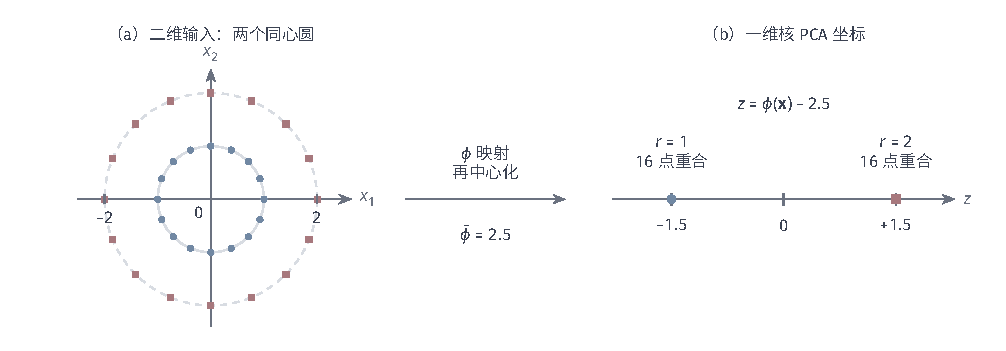
\includegraphics[width=169.000mm]{figures/04-classic-models/00-shared/tikz/dim-kernel-radial/figure.pdf}
  \caption{由核选择保留量的构造例子。左图在半径为$1,2$的圆上各取16个等角度样本，圆点与方点区分两圈。所示特制核对应标量特征$\phi(\bm{x})=\lVert\bm{x}\rVert_2^2$，中心化核矩阵秩为1；选择图示主轴方向，核PCA坐标为$\pm1.5$。右侧每个标记表示16点重合，坐标无量纲。此结果依赖所选核，不能推广为任意高斯核或多项式核的输出。}
  \label{fig:dim-kernel-radial}
\end{figure*}

新样本必须沿用训练特征均值，才能与训练表示处于同一坐标系。令$\bm{k}(\bm{x})_i=K(\bm{x}_i,\bm{x})$，中心化及投影为
\begin{equation}
  \label{eq:dim-kpca-extension}
  \begin{aligned}
    \bm{k}_{\mathrm{c}}(\bm{x})
      ={}&\bm{k}(\bm{x})-\frac1n\bm{K}\bm{1}\\
         &-\frac1n\bm{1}\bm{1}^{\top}\bm{k}(\bm{x})
          +\frac1{n^2}\bm{1}\bm{1}^{\top}\bm{K}\bm{1},\\
    z_\ell(\bm{x})
      ={}&\bm{\alpha}_\ell^{\top}\bm{k}_{\mathrm{c}}(\bm{x}).
  \end{aligned}
\end{equation}
两个减项分别扣除与训练均值的内积，末项补回均值自内积。只减新核向量自身均值会漏掉这些量；加入新点重算均值，则是在改变原先的映射。

高斯核带宽过大时，各核值接近，中心化信号变弱；带宽过小时，核矩阵接近单位阵，主方向难以辨认。距离中位数可作初始尺度，再用任务验证选择。监督任务中的中心化和主方向均应在训练折拟合。

对当前训练点，误差相应为$n^{-1}\sum_{j>k}\lambda_j^{\mathrm K}$，所以保留中心化核矩阵的全部正谱能够精确重构训练特征，却未必提供低维压缩。

\subsubsection{理论分析}
\label{sec:dim-kpca-theory}

\paragraph{表达能力}
核PCA的候选重构仍是线性的，但线性子空间位于$\mathcal H$中。若$\mathcal H$可分且$\mathbb E K(\bm X,\bm X)<\infty$，总体特征协方差的有序特征值记为$\lambda_j^{\mathcal H}$，同样的正交分解给出最佳$k$维特征重构误差$\sum_{j>k}\lambda_j^{\mathcal H}$。只有中心化特征以概率一位于一个至多$k$维的子空间中，该误差才为零；输入由$k$个参数控制，并不自动满足这个核特征秩条件。

相对于原输入的非线性来自核映射，核也可能先丢掉信息。图\ref{fig:dim-kernel-radial}的径向核只保留半径，所有同半径点的编码相同，保留再多主方向也不能恢复角度。即使核映射可区分不同输入，有限维截断仍可能合并它们；特征重构点还不一定属于$\bm\phi(\mathbb R^d)$。因此特征误差小是否意味着原空间误差小，需要可逆性及逆映射稳定条件，不能仅由核技巧推出。

\paragraph{收敛性}

固定正定核后，经验方差目标可由谱分解全局求解，核矩阵近似及求谱精度决定数值误差。相同谱计算还连接点间距离：第\ref{sec:dim-mds}节定义经典MDS后，引理\ref{thm:dim-kpca-mds}将证明核诱导距离与中心化核PCA给出相同训练坐标。该联系针对特征距离，局部重构和图平滑则使用不同目标。

\paragraph{泛化性}
核PCA的新点公式定义了共享编码，期望风险则应按它实际优化的特征重构来评价。

\begin{theorem}[核PCA在有界核条件下的期望特征重构风险界]
 \label{thm:dim-kpca-risk}
设训练样本独立同分布于$P$，核在训练前固定、特征空间$\mathcal H$可分，且
$K(\bm x,\bm x)\leq\kappa^2$几乎处处。总体特征均值为$\bm m=\mathbb E\bm\phi(\bm X)$，训练特征均值为$\widehat{\bm m}$，所学秩$k$正交投影为$\widehat{\mathcal P}$。固定重构规则
$\widehat r_{\mathcal H}(\bm x)=\widehat{\bm m}
 +\widehat{\mathcal P}(\bm\phi(\bm x)-\widehat{\bm m})$后，定义
\[
 R_{\mathcal H,n}
 =\mathbb E_{\bm X\sim P}
   \lVert\bm\phi(\bm X)-\widehat r_{\mathcal H}(\bm X)\rVert_{\mathcal H}^2.
\]
新点独立于训练集。记$R_{\mathcal H,k}^\star$为以总体均值中心化后的最佳秩$k$投影风险，$e_n$为经验特征重构距全局最优的差。则
\begin{equation}
 \mathbb E_{D_n}R_{\mathcal H,n}
 \leq R_{\mathcal H,k}^\star
       +\frac{8\sqrt{k}\,\kappa^2}{\sqrt n}
       +\frac{4(2\sqrt{k}+1)\kappa^2}{n}
       +\mathbb E_{D_n}e_n.
 \label{eq:dim-kpca-risk}
\end{equation}
\end{theorem}

证明沿用定理\ref{thm:dim-pca-risk}：$\lVert\bm\phi(\bm X)-\bm m\rVert_{\mathcal H}\leq2\kappa$，有限矩阵的Frobenius范数换成协方差算子的Hilbert--Schmidt范数，即算子奇异值平方和的平方根；独立平均、均值校正和秩$k$投影的估计仍相同。取$r=2\kappa$便得到该界，特征空间不必有限维。核PCA的重构风险也有更细致的专门分析\scite{blanchard2007kpca}

经验协方差逼近总体协方差，使经验最佳投影的总体特征损失接近该族最佳值，这是风险转移所需的链路；谱隙只在进一步估计主子空间时需要。数据自适应核需另外控制核选择，不能将固定核界原样使用。式\eqref{eq:dim-kpca-risk}也不保证原输入重构：截断特征可能没有原像，原像算法还需独立误差分析。

\subsubsection{优化计算能力}

常用核的全矩阵构造约需$O(n^2d)$，存储为$O(n^2)$，稠密谱分解为$O(n^3)$。Nystr\"om近似使用代表列减少矩阵计算，随机Fourier特征则对合适的平移不变核构造有限特征后再做线性PCA。近似误差需要单独评价，适用核也各有条件。

两种近似处理的对象不同：代表列概括训练样本间的核关系，随机特征直接给输入一个有限维映射。前者仍依赖代表样本的覆盖，后者需要选择特征数；省去全核计算的同时，应检查近似后的谱方向与新点编码是否仍保留所需变化。

\subsubsection{小结}

核PCA先用核规定特征几何，再按方差选择该空间中的主方向。它能够让某些原空间非线性关系进入线性表示，却也可能在核映射时丢掉角度等信息；选核与选择保留维数因而回答不同问题。新样本须沿用训练中心化与核投影，原空间重构还需处理原像问题。

全核矩阵成为瓶颈时，代表列近似减少处理的样本方向，有限随机特征则对适用核先构造显式映射。两者节省不同计算，也引入不同近似。应同时比较核几何、近似精度和新点计算，不能把特征空间方差的改善直接解释为原输入重构或下游预测改善。

\subsection{模型对比与总结}
\label{sec:dim-linear-comparison}

同一组线性坐标可以为不同信息服务。PCA按输入方差选方向，适合保留主要变化；若大方差来自单侧噪声或任务无关因素，这一准则就没有理由优先保留所需信息。CCA让配对视图的共同变化决定方向，PLS与判别投影让响应或类别参与方向选择。它们改变的是选择方向的依据，输入、输出和验证数据也因此需要相应调整。

ICA进一步改变了要分离的统计关系。PCA的正交方向让得分不相关，但不相关仍可能包含非线性依赖；ICA用独立源假设及非高斯信息寻找解混方向。这里的任务是分离来源，标准方形ICA并不自动减少维数。源假设不成立时，换一个对比函数也不能保证得到真实来源。

重构方法的差别还在允许怎样组合基。PCA对全部样本使用一个正交子空间；稀疏PCA限制编码需要读取的变量，RPCA则把共享低秩信号与稀疏污染分开。NMF要求成分只作非负叠加，稀疏编码允许较大的字典和正负组合，再以稀疏约束控制每个样本的活跃原子。非负、稀疏、正交与异常污染分别约束不同对象，应按成分含义和污染方式组合，不能把一种约束当成其他要求的替代。

原空间的线性方向不够时，核PCA先改变观察输入的特征几何，再按该空间的方差选择方向。随机投影则省去数据方向的拟合，以固定随机矩阵压缩点间距离信息；它没有以最大方差或最小重构残差选择矩阵。表\ref{tab:dim-linear-comparison}把这些目标与新点编码并列，便于区分表示要保留什么，以及训练后怎样复用它。

\begin{table*}[htbp]
  \centering
  \small
  \begin{tabularx}{\linewidth}{@{}l>{\RaggedRight\arraybackslash}X>{\RaggedRight\arraybackslash}X>{\RaggedRight\arraybackslash}X@{}}
    \toprule
    方法 & 主要目标与约束 & 新样本的表示 & 典型边界\\
    \midrule
    PCA & 正交投影下保留方差 & 中心化后矩阵乘法 & 对尺度、异常值敏感\\
    CCA & 配对视图的相关性最大 & 两侧分别线性投影 & 需配对观测，易过拟合相关性\\
    ICA & 独立源的线性解混 & 白化及解混乘法 & 独立性、非高斯性与可识别性\\
    NMF & 非负基与非负系数重构 & 非负约束推断 & 非凸、通常不唯一\\
    稀疏编码 & 少量原子重构观测 & 稀疏优化 & 可为高维编码，需控制推断成本\\
    随机投影 & 随机矩阵近似保距 & 固定矩阵乘法 & 维数、误差与失败概率的权衡\\
    核PCA & 特征空间方差 & 训练中心化核投影 & 核几何、样本展开与原空间重构\\
    \bottomrule
  \end{tabularx}
  \caption{线性投影与线性组合方法的比较。目标成立均依赖各小节的具体条件；“新样本可编码”不等于编码具有统计泛化保证。}
  \label{tab:dim-linear-comparison}
\end{table*}

求解方式进一步决定预算。谱分解类方法主要处理协方差或数据矩阵，迭代拟合还需计入稀疏结构、停止精度与总轮数，固定映射则需计入生成和使用矩阵的成本。基可以追溯原始特征，是否对应可解释概念仍要由数据和任务验证。

选择线性组合时，先确定要保留的信息和新样本的编码方式。若还需解释各特征的测量误差，可转向第\ref{sec:dim-probabilistic}节的生成模型；只有对象差异时，下一节将讨论如何从距离安排坐标。原空间线性基不足以描述弯曲结构时，还需要改变特征或关系。

\section{基于距离的降维}
\label{sec:dim-distance}

对象之间的差异有时比原始坐标更容易取得，例如相似性评分或编辑距离。此时需要根据差异安排位置，而非直接投影特征。多维缩放提供了这种坐标恢复；下一节还会把差异限制到局部邻域，用来研究弯曲几何。

\subsection{多维缩放（MDS）}
\label{sec:dim-mds}

有时我们只有对象之间的差异，没有每个对象的向量坐标。例如，受试者可以评价两种气味有多相似，却不一定能为每种气味给出同一组数值属性；PCA因而缺少可以投影的坐标矩阵。\term{多维缩放}（multidimensional scaling, MDS）从点对差异反求低维位置，让这些位置的几何关系尽量符合输入。Young与Householder于1938年研究距离对坐标的代数约束，为坐标恢复建立了几何依据\scite{dimYoung1938}差异不一定能精确表示为指定维数中的欧氏距离，因此目标还需要规定允许怎样的失真。

Torgerson在1952年系统提出经典MDS时，还要处理心理距离怎样测量。刺激比较的差异可能缺少确定零点，因此原工作先估计比较距离中的未知加性常数，再分析维数和刺激坐标\scite{dimTorgerson1952}差异输入本身也有测量假设，这里的加性常数与下面的坐标、核矩阵中心化承担不同作用。

\subsubsection{模型结构}

将对象差异记为对称矩阵$\bm{D}\in\mathbb{R}^{n\times n}$，要求$\bm{D}_{i,j}\geq0$、$\bm{D}_{i,i}=0$。它可以来自欧氏、编辑、图距离或人工评分；这些关系未必能在指定维数中由欧氏距离实现。MDS的拟合准则决定采用哪一种近似。

要恢复欧氏几何，可以先从距离平方求中心化内积。\term{经典MDS}（classical MDS）采用这一转换，令$\bm{1}\in\mathbb{R}^n$为全一向量、$\bm{I}_n$为单位矩阵：
\begin{equation}
  \label{eq:dim-mds-centering}
  \begin{aligned}
    \bm{H}&=\bm{I}_n-\frac{1}{n}\bm{1}\bm{1}^{\top},\\
    \bm{D}^{\circ2}_{i,j}&=(\bm{D}_{i,j})^2,\\
    \bm{B}&=-\frac12\bm{H}\bm{D}^{\circ2}\bm{H}.
  \end{aligned}
\end{equation}
$\circ2$是逐元素平方。左右乘$\bm{H}$分别扣去列、行均值，即双中心化；欧氏输入得到的$\bm{B}$是中心化坐标的Gram矩阵，记录两两内积且为半正定。

从$\bm{B}$的正谱取得实数坐标。记$\lambda_1\geq\cdots\geq\lambda_r>0$，相应欧氏单位特征向量为$\bm{u}_1,\ldots,\bm{u}_r$；选择$k\leq r$后，坐标为
\begin{equation}
  \label{eq:dim-mds-coordinates}
  \bm{Z}=\bm{U}_k\bm{\Lambda}_k^{1/2},
  \qquad
  \bm{Z}_{i,\ell}=\sqrt{\lambda_\ell}\,(\bm{u}_\ell)_i.
\end{equation}
$\bm{U}_k$收集所选特征向量，$\bm{\Lambda}_k$收集相应特征值。其平方根缩放使坐标内积逼近$\bm{B}$，最小化的内积残差称为strain：
\begin{equation}
  \label{eq:dim-mds-strain}
  \min_{\substack{\bm{Z}\in\mathbb{R}^{n\times k}\\
                  \bm{Z}^{\top}\bm{1}=\bm{0}}}
  \left\lVert\bm{B}-\bm{Z}\bm{Z}^{\top}\right\rVert_{\mathrm{F}}^2.
\end{equation}
非欧氏差异可能使$\bm{B}$含负特征值。半正定秩约束近似舍弃负谱，保留最大的至多$k$个正特征值；这种内积近似通常也会改变输入距离。

\paragraph{距离残差目标}
任务若直接比较距离数值，可以让\term{度量MDS}（metric MDS）最小化距离残差。给定对称非负权重$w_{i,j}$，记$\delta_{i,j}(\bm{Z})=\lVert\bm{z}_i-\bm{z}_j\rVert_2$，常用应力（stress）目标为
\begin{equation}
  \label{eq:dim-mds-stress}
  S(\bm{Z})
  =\sum_{i<j}w_{i,j}
    \bigl(\delta_{i,j}(\bm{Z})-\bm{D}_{i,j}\bigr)^2.
\end{equation}
strain比较内积，stress比较距离。虽然距离与中心化内积可互相转换，两种残差平方和仍有不同的最优近似。有些文献也将经典MDS称为metric scaling，本章按实际目标区分。

\subsubsection{参数学习}

经典MDS的平方Frobenius目标可以沿正交特征方向分解。半正定约束排除负谱，秩约束保留较大的正谱，因此双中心化和谱截断给出全局最优表达；特征向量仍需数值求解。

应力型MDS可用梯度法、拟牛顿法，或\term{SMACOF}（scaling by majorizing a complicated function）。SMACOF在当前坐标构造与目标相切的二次上界，再最小化该上界；记上界为$Q$，下降关系为
\[
  S(\bm{Z}^{(s+1)})
  \leq Q(\bm{Z}^{(s+1)}\mid\bm{Z}^{(s)})
  \leq Q(\bm{Z}^{(s)}\mid\bm{Z}^{(s)})
  =S(\bm{Z}^{(s)}).
\]
目标非负且不增加时，目标值收敛；迭代点是否到达驻点、极小或全局最优仍要另查。实践中可以用经典MDS初始化并比较多次运行，SMACOF的构造与实现见de Leeuw和Mair的系统介绍\scite{dimDeLeeuw2009}

\subsubsection{理论分析}
\label{sec:dim-mds-theory}

\paragraph{表达能力}
给定对称非负差异矩阵$\bm D$及零对角，所有距离能在$k$维欧氏坐标中精确实现，当且仅当式\eqref{eq:dim-mds-centering}的$\bm B$半正定且秩至多为$k$。必要性来自$\bm B=\bm Z\bm Z^\top$；反过来对这样的$\bm B$作谱分解即可构造坐标，再以$D_{i,j}^2=B_{i,i}+B_{j,j}-2B_{i,j}$恢复原距离。因此真实低维欧氏点集可以零失真重现，含负谱的相异度却不能靠增加有限的欧氏维数消除失真。

经典MDS对内积的最佳平方残差也可以直接读出：保留$\bm B$最大的至多$k$个正特征值后，最小strain为“所有负特征值的平方和，加上未保留正特征值的平方和”。负谱反映非欧氏性，正谱尾部反映维数不足，两者不是求解误差。应力型MDS直接拟合距离，数值最优值通常不同。即使全部距离精确，坐标还允许整体平移、旋转及反射，距离本身无法恢复原特征轴。

\paragraph{收敛性}

经典MDS的全局最优针对内积目标；应力型MDS的迭代通常在适当条件下保证下降。要进一步联系PCA，需要让两者处理同一批欧氏观测，并比较同一中心化坐标的谱截断。

设$\bm{D}$来自坐标矩阵$\bm{X}$各行的欧氏距离，中心化坐标为$\bm{X}_{\mathrm{c}}=\bm{H}\bm{X}$。平移不改变这些距离，双中心化得到
\[
  \bm{B}=\bm{H}\bm{X}\bm{X}^{\top}\bm{H}
  =\bm{X}_{\mathrm{c}}\bm{X}_{\mathrm{c}}^{\top}.
\]
该Gram矩阵来自中心化后的$\bm{X}_{\mathrm{c}}$。选择相同维数和相应奇异方向时，PCA与经典MDS共享谱截断；证明的关键是展开距离平方，说明双中心化怎样消去平移项并恢复该Gram矩阵。

\begin{theorem}[经典MDS在欧氏距离下的全局最优解]
  \label{thm:dim-mds-pca}
  设$\bm{X}^{\top}\bm{1}=\bm{0}$，$\bm{D}_{i,j}=\lVert\bm{x}_i-\bm{x}_j\rVert_2$，且$1\leq k\leq\operatorname{rank}(\bm{X})$。若PCA与经典MDS选取相互对应的前$k$个奇异方向，则两者的坐标都可取为$\bm{U}_k\bm{\Sigma}_k$，从而得到相同的坐标Gram矩阵$\bm{U}_k\bm{\Sigma}_k^2\bm{U}_k^{\top}$。同一所选子空间内的坐标可相差右侧正交变换，而Gram矩阵保持不变。
\end{theorem}
\begin{proof}
  令$\bm{a}\in\mathbb{R}^n$满足$a_i=\lVert\bm{x}_i\rVert_2^2$。展开距离平方并双中心化，得到
  \[
    \begin{aligned}
      \bm{D}^{\circ2}
        &=\bm{a}\bm{1}^{\top}+\bm{1}\bm{a}^{\top}
          -2\bm{X}\bm{X}^{\top},\\
      \bm{B}
        &=\bm{H}\bm{X}\bm{X}^{\top}\bm{H}
         =\bm{X}\bm{X}^{\top}.
    \end{aligned}
  \]
  第一、第二项消失，是因为$\bm{H}\bm{1}=\bm{0}$；末步使用样本已经中心化。对薄奇异值分解$\bm{X}=\bm{U}\bm{\Sigma}\bm{V}^{\top}$，有$\bm{B}=\bm{U}\bm{\Sigma}^2\bm{U}^{\top}$。MDS坐标与PCA得分因而分别为
  \[
    \bm{Z}_{\mathrm{MDS}}=\bm{U}_k\bm{\Sigma}_k,
    \qquad
    \bm{X}\bm{V}_k=\bm{U}_k\bm{\Sigma}_k.
  \]
  在同一所选子空间内旋转坐标轴不改变Gram矩阵。
\end{proof}

等价对象是同一保留维数$k$下的中心化坐标Gram矩阵及其诱导距离，原特征轴并未恢复。只有$k=\operatorname{rank}(\bm{X}_{\mathrm{c}})$、保留全部正特征值时，坐标才保留全部输入欧氏距离；$k<\operatorname{rank}(\bm{X}_{\mathrm{c}})$时，两者共享一个改变原距离的谱截断。

截断若满足$\lambda_k=\lambda_{k+1}$，可以选择不同的最优部分子空间，结果未必只差一个$k$维旋转。小谱隙也使方向对距离扰动敏感；评价稳定性时可比较对齐坐标、子空间或重构距离。

核特征距离也具有同一内积展开，因而第\ref{sec:dim-kpca}节预告的联系可以按相同方式证明。

\begin{lemma}[核诱导距离下的等价关系]
  \label{thm:dim-kpca-mds}
  设$K$为正定核，记$\bm{K}_{i,j}=K(\bm{x}_i,\bm{x}_j)$。训练点间的特征距离为
  \[
    \bm{D}_{i,j}^2
    =\bm{K}_{i,i}+\bm{K}_{j,j}-2\bm{K}_{i,j}.
  \]
  对此距离进行经典MDS，与对$\bm{K}$进行中心化核PCA，在选择相同正特征子空间和归一化后给出相同训练坐标。重特征值和截断处的非唯一性与定理\ref{thm:dim-mds-pca}相同。
\end{lemma}
\begin{proof}
  令向量$\bm{a}$的元素$a_i=\bm{K}_{i,i}$，距离平方矩阵为$\bm{a}\bm{1}^{\top}+\bm{1}\bm{a}^{\top}-2\bm{K}$。双中心化消去前两项，得到$\bm{B}=\bm{H}\bm{K}\bm{H}=\bm{K}_{\mathrm{c}}$。式\eqref{eq:dim-mds-coordinates}与式\eqref{eq:dim-kpca-training}因而输出相同的$\bm{U}_k\bm{\Lambda}_k^{1/2}$。
\end{proof}

\paragraph{泛化性}
经典MDS在给定点集上恢复坐标，评价独立新对象时还需规定坐标扩展与重构方式。距离来自欧氏观测、且使用同一训练中心时，可以借助它与PCA的等价关系得到下面的风险结论。

\begin{theorem}[经典MDS在有界欧氏观测下的期望重构风险界]
 \label{thm:dim-mds-risk}
若距离恰好来自独立同分布的欧氏观测，且$\lVert\bm X-\bm\mu\rVert_2\leq r$，经典MDS及下述固定中心扩展与PCA给出相同的子空间坐标。将坐标与原欧氏空间对齐，并用该子空间重构新点，其风险因此满足
\[
 \mathbb E_{D_n}R_{\mathrm{MDS},n}
 \leq R_k^\star+2\sqrt{k}\,r^2/\sqrt n
                  +(2\sqrt{k}+1)r^2/n+\mathbb E e_n,
\]
其中$e_n$为谱求解的经验重构误差，结论由定理\ref{thm:dim-pca-risk}及PCA--MDS等价关系得到。它要求真实欧氏距离与同一训练中心，测量误差或非欧氏差异不满足这一设定。

\end{theorem}

只有固定差异矩阵时，可以合法评价的对象是该矩阵上的点对损失。度量MDS按$w_{ij}/\sum_{a<b}w_{ab}$抽取一对对象，平方距离残差的期望为
$R_G(\bm Z)=S(\bm Z)/\sum_{a<b}w_{ab}$。
若学习器的完整应力距全局最小值至多为$e_G$，便有
$R_G(\widehat{\bm Z})\leq\inf_{\bm Z}R_G(\bm Z)+e_G/\sum_{a<b}w_{ab}$。
这里是有限对象集上的关系风险，并无独立新对象的保证；经典MDS则最小化内积残差，不能将其谱最优性改称距离应力最优。


新对象到训练对象的距离已知时，可以固定原坐标作经典MDS扩展。记这些距离平方为$s_i$，$\bar s=n^{-1}\sum_i s_i$；训练距离的行均值为$r_i=n^{-1}\sum_j\bm{D}_{i,j}^2$，总均值为$\bar r=n^{-1}\sum_i r_i$。相对训练中心的内积与坐标为
\begin{equation}
  \label{eq:dim-mds-extension}
  \begin{aligned}
    b_i&=-\frac12(s_i-\bar s-r_i+\bar r),\\
    \bm{z}(\bm{x})
      &=\bm{\Lambda}_k^{-1/2}\bm{U}_k^{\top}\bm{b}.
  \end{aligned}
\end{equation}
第一行沿用训练中心计算内积，第二行用最小二乘取得相应坐标。训练点保持固定，与加入新点重做MDS的结果不同；非欧氏差异下，该扩展是相对已有表示的近似投影\scite{dimBengio2003}

\subsubsection{优化计算能力}

完整稠密经典MDS需要$O(n^2)$存储，谱分解通常为$O(n^3)$。部分谱或Nystr\"om近似可以减少计算；标志点MDS先嵌入代表点，再按到代表点的距离扩展，近似质量依赖代表点的覆盖。

\subsubsection{支持距离数值保持场景}

若评价直接针对对象间的距离误差，就应采用式\eqref{eq:dim-mds-stress}的应力目标，而不是内积残差。前述SMACOF等方法用于求解这一目标；相同的输入距离和输出维数下，它与经典MDS仍可能给出不同坐标，因为两者所衡量的失真不同。

\subsubsection{支持差异顺序保持场景}

当差异顺序比数值更可信时，\term{非度量MDS}（nonmetric MDS）用非递减函数$g(\bm{D}_{i,j})$作为式\eqref{eq:dim-mds-stress}中的目标距离，同时估计$g$和$\bm{Z}$。尺度约束排除共同缩到零的退化，保序要求作用于拟合差异；有限维坐标仍可能无法满足所有严格次序。Kruskal于1964年将顺序信息与应力准则结合\scite{dimKruskal1964}

非度量MDS可以交替求保序回归和坐标更新。它放宽了距离数值，只要求拟合后的次序，但低维点集仍须满足相应的几何关系。

\subsubsection{支持局部距离优先保持场景}

距离残差通常采用迭代拟合，也可以按距离选择权重。例如所有非对角距离$\bm{D}_{i,j}>0$时，\term{Sammon映射}使用
\begin{equation}
  \label{eq:dim-sammon}
  S_{\mathrm{Sammon}}(\bm{Z})
  =\frac{1}{\sum_{i<j}\bm{D}_{i,j}}
    \sum_{i<j}
    \frac{\bigl(\delta_{i,j}(\bm{Z})-\bm{D}_{i,j}\bigr)^2}
         {\bm{D}_{i,j}}.
\end{equation}
小距离的相同绝对误差在此受到更大惩罚，使局部距离更受重视。它仍是近似目标，零差异需要合并对象或另定权重\scite{dimSammon1969}

\subsubsection{小结}

MDS根据对象差异安排坐标，选择时需明确要保留内积、距离还是顺序。目标维数、差异的来源及矩阵规模共同影响可用表示；新对象还需按固定参考坐标扩展。

\subsection{模型对比与总结}

距离法的共同输入是对象差异，主要分歧在允许改变什么。经典MDS把距离平方转成中心化内积，再作谱近似；这与PCA从坐标协方差提取方向相联系，但前者可以直接接收差异矩阵。任务若关心距离数值的误差，度量MDS改为拟合点对距离，谱截断因而不再直接完成所选目标的求解。

非度量MDS进一步放松距离数值，只要求拟合差异保留可信顺序。它适合顺序比数值尺度更可靠的输入，同时增加保序函数的估计；这一放松也会舍弃绝对差异大小的信息。Sammon映射仍比较距离数值，但让较短距离的同等绝对误差承担更大代价，回应全局平方误差可能弱化局部距离的问题。

计算规模与拟合准则是另一组取舍。部分谱、矩阵近似和标志点减少需要处理的方向或点对，不能修正不适合任务的差异来源，也不能消除目标维数带来的失真。比较这些方法时，应先固定同一批差异和保留要求，再比较相应的失真、样本外定位和计算预算；内积残差、距离应力与保序误差的数值不能直接排名。

\section{基于邻域的降维}
\label{sec:dim-neighbors}
\label{sec:dim-manifold}

如果原空间距离主要在小范围内可信，可以先建立邻域，再组织全局坐标。第\ref{sec:classic-overview-neighborhood}节给出了邻域与图的共同机制；这里按要保留的关系展开：图路径描述长度，局部组合描述重构，图上平滑和随机游走描述连通性，邻居概率或边权则用于安排可观察的布局。

几何方法中的部分模型假设数据接近\term{流形}（manifold），即局部可以用少量连续坐标描述的空间。弯曲结构的方向随位置改变，直接投影可能混合沿曲面相距较远的点；局部自由度少，整体却仍可能无法在同维数中无失真展开。各方法需要的采样和几何条件将在具体构造中给出。

以下继续使用$n,d,k,m,q$与$\bm{X},\bm{Z}$。布局的输入距离记为$\delta_{i,j}=\lVert\bm{x}_i-\bm{x}_j\rVert_2$，低维距离记为$r_{i,j}=\lVert\bm{z}_i-\bm{z}_j\rVert_2$。训练坐标是这些方法直接求得的对象，接收新样本还需规定相应映射或扩展。

\subsection{等距映射（Isomap）}
\label{sec:dim-isomap}

把一张平面纸卷起来，纸上原本相隔很远的两点可能隔着相邻卷层靠得很近。若MDS直接保留卷起后的直线距离，就会把这两点也放得很近，难以恢复展开时的关系。沿纸面行走的最短长度则保留了这种关系；在一般流形上，这一长度称为\term{测地距离}（geodesic distance），记为$d_{\mathcal{M}}$。\term{等距映射}（isometric mapping, Isomap）先只连接局部邻居，再以图中的最短路径估计测地距离，最后交给经典MDS恢复坐标。Tenenbaum、de Silva与Langford于2000年提出了该方法\scite{dimTenenbaum2000}它改变了MDS的距离输入；邻域若误连相邻卷层，图上的捷径仍会破坏这一估计。

\subsubsection{模型结构}

将样本作为顶点建立无向图$\mathcal{G}=(V,E)$，连接距离不超过$\varepsilon$的点，或对称化$q$近邻。近邻并集与互近邻给出的边不同，需要明确采用哪一种。每条边的长度为$\ell_{i,j}=\lVert\bm{x}_i-\bm{x}_j\rVert_2$，是路径成本；长度越小越近，与后文连接越强数值越大的相似度权重不同。

路径只能沿图中边行走。将一条路径的边长相加，再在全部可行路径中选择最短者：
\begin{equation}
  \label{eq:dim-isomap-distance}
  d_{\mathcal{G}}(i,j)
  =\min_{\substack{i=i_0,\ldots,i_s=j\\(i_{a-1},i_a)\in E}}
    \sum_{a=1}^{s}\ell_{i_{a-1},i_a}.
\end{equation}
由全部图距离组成$\bm{D}_{\mathcal{G}}$，计算$\bm{B}_{\mathcal{G}}=-\tfrac12\bm{H}\bm{D}_{\mathcal{G}}^{\circ2}\bm{H}$，再按式\eqref{eq:dim-mds-coordinates}取坐标。局部连接、全局路径和欧氏表示依次承担三项工作；路径近似与MDS拟合也分别引入误差。

邻域决定路径能否合理近似曲面长度。图\ref{fig:dim-geodesic}中的两段曲线在观测空间接近，沿曲线却相距很远；跨过弯曲部分的一条错误边，可能缩短许多点对的图距离。
\begin{figure}[htbp]
  \centering
  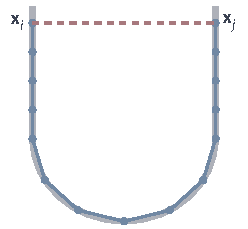
\includegraphics[width=42.012mm]{figures/04-classic-models/00-shared/tikz/dim-geodesic/figure.pdf}
  \caption{一维弯曲曲线上的距离示意。曲线表示嵌入观测空间的一维流形，曲线上的点表示离散样本；沿相邻样本连接的折线表示邻域图路径，其各段长度之和用于近似沿曲线的测地距离。顶部红色虚线是两点间的欧氏直线；若邻域取值过大而把它误纳入图中，就会形成穿过流形外部、低估测地距离的短路。图为几何示意，不是算法输出或实验结果，未给出数值误差。}
  \label{fig:dim-geodesic}
\end{figure}

\subsubsection{参数学习}

暴力建邻域约需$O(n^2d)$时间，空间索引的收益依赖维数与分布。非负边长下，从每点运行二叉堆Dijkstra的成本为$O(n(|E|+n)\log n)$，Floyd--Warshall为$O(n^3)$。后续稠密MDS仍需$O(n^2)$存储、通常$O(n^3)$的完整谱分解；稀疏邻域并未使全体点对距离也稀疏。

输入度量、预处理、$q$或$\varepsilon$以及$k$共同决定结果。小邻域可能断连，大邻域可能跨过卷层，噪声和非均匀采样也会改变可用尺度。可检查连通分量、边长分布及随邻域变化的稳定性。距离相关残差$1-R^2$提供辅助诊断，但对统一缩放不敏感，仍需直接检查失真与测地近似。

\subsubsection{理论分析}
\label{sec:dim-isomap-theory}

\paragraph{表达能力}
Isomap能精确表示的理想对象，是测地距离本来就等于某个$k$维欧氏区域中直线距离的流形。例如一张无拉伸卷起的纸，若参数区域凸，最短纸面路径对应展开后的直线段；图距离恰好等于测地距离时，MDS可以恢复这些展开坐标；图距离仅近似准确时，坐标也仍有相应的近似误差。凸性在这里保证两点之间的直线段没有离开参数区域。带孔区域中的最短路可能绕过孔洞，即使局部平坦，全局测地距离也未必等于展开坐标的直线距离。

并非每个低维流形都有这种全局欧氏表示。取圆周上的四个等间隔点，沿圆的相邻距离为$a>0$、相对点距离为$2a$。若欧氏坐标精确保留这些距离，两条长度为$a+a$的路径都必须满足三角不等式取等；两个中间点便都成为同一线段的中点。但它们在圆周上相距$2a$，产生矛盾。因此即使图距离恰好等于真实圆周测地距离，任何欧氏维数也不能同时零失真实现全部点对。实际Isomap还会叠加邻域短路、覆盖不足及MDS截断的误差；前两项改善后，后一项的几何限制仍然存在。

\paragraph{收敛性}
固定图后，最短路径算法求出图距离，经典MDS求相应的谱近似。数值精度可以通过路径与谱求解检查，邻域是否近似真实几何则属于建模条件；计算完成并未消除两层近似的误差。

\paragraph{泛化性}
样本增加时，希望图距离也越来越接近测地距离。覆盖不足会漏掉必要连接，边长失真过大又会形成捷径，下面的确定性界分别控制这两种问题。

覆盖空隙$h$衡量流形上各位置到最近样本的最大测地距离，单边失真$\eta$衡量弦长比测地距离短多少。证明沿最短测地线放置分割点，再用附近样本替代它们，构造图路径以控制误差；这里尚未要求该距离能嵌入指定$k$维。

\begin{lemma}[覆盖条件下的图距离界]
  \label{thm:dim-isomap-bound}
  设$\mathcal{M}\subset\mathbb{R}^d$连通，任意两点间存在最短测地线。样本的测地填充距离为
  \[
    h=\sup_{\bm{x}\in\mathcal{M}}\min_i
      d_{\mathcal{M}}(\bm{x},\bm{x}_i).
  \]
  图连接全部欧氏距离不超过$\varepsilon$的样本对，并以欧氏弦长为边长。假设$h<\varepsilon/2$，且存在$0\leq\eta<1$，使每条边都满足
  \[
    \lVert\bm{x}_i-\bm{x}_j\rVert_2
    \geq(1-\eta)d_{\mathcal{M}}(\bm{x}_i,\bm{x}_j).
  \]
  则对所有样本对，图距离有限，且
  \begin{equation}
    \label{eq:dim-isomap-bound}
    \begin{aligned}
      d_{\mathcal{G}}(i,j)
        &\geq(1-\eta)d_{\mathcal{M}}(\bm{x}_i,\bm{x}_j),\\
      d_{\mathcal{G}}(i,j)
        &\leq\left(1+\frac{2h}{\varepsilon-2h}\right)
          d_{\mathcal{M}}(\bm{x}_i,\bm{x}_j).
    \end{aligned}
  \end{equation}
\end{lemma}
\begin{proof}
  对任意图路径，各边弦长至少是对应测地距离的$1-\eta$倍。将其相加，再用测地距离的三角不等式，就得到下界。

  为证明上界，记两端点的测地距离为$L$，取连接它们的一条最短测地线，令$a=\varepsilon-2h>0$。若$L=0$，结论成立；否则沿测地线每隔$a$放一个分割点，末段不足$a$，总段数为$s=\lceil L/a\rceil$。保留原来的两个样本端点，把每个内部分割点替换成测地距离不超过$h$的样本。相邻替代样本的测地距离至多$a+2h=\varepsilon$，欧氏距离不更大，因此构成图中的边；重复样本可略去。

  每个内部分割点的替代误差至多在两条相邻边中各计一次，而两端点无需替代，故所构造路径的长度至多
  \[
    L+2h(s-1)
    \leq L+\frac{2hL}{\varepsilon-2h}.
  \]
  图最短路径不长于这条路径，得到上界，同时证明图中这些端点相连。
\end{proof}

对一列样本与邻域，若$h/\varepsilon\to0$且$\eta\to0$，两侧界给出样本点对上的统一相对距离一致性。曲率有界仍需配合足够小的邻域尺度，才能排除卷层间连接。若采样独立且密度有正下界，可以研究覆盖空隙$h$的概率界，条件还需包括体积、内在维数、覆盖数和密度。

还可以把覆盖条件转成新点对的期望风险。

\begin{theorem}[Isomap在覆盖与无短路条件下的期望测地距离误差界]
 \label{thm:dim-isomap-risk}
设$\mathcal M$紧致，测地直径至多为已知常数$D$；训练样本独立同分布于$P$，$P$的支持为$\mathcal M$。假设流形上任意欧氏距离不超过$\varepsilon$的点对均满足前述图距离引理中的无短路条件。对独立新点$\bm x,\bm x'$，冻结训练边，将两个查询节点按同一半径接入图，并保留满足半径条件的查询间边；以该图的最短路径$d_n(\bm x,\bm x')$预测测地距离。为使覆盖失败时的风险也有限，取$\widehat d_n=\min\{d_n,D\}$，不连通时约定$\widehat d_n=D$。

用$N_h$个测地半径$h/2$的球覆盖$\mathcal M$，并假设每个覆盖球的$P$质量至少为$p_h>0$，其中$h<\varepsilon/2$。任一球未包含训练点的概率至多为$e^{-np_h}$；所有球均有样本时，填充距离至多为$h$。查询节点加入后仍保持这一覆盖，引理\ref{thm:dim-isomap-bound}给出新点对上的距离误差。因此，令
$\beta_h=\max\{\eta,2h/(\varepsilon-2h)\}$，有
\begin{equation}
 \mathbb E_{D_n}\mathbb E_{\bm X,\bm X'\sim P}
  [\widehat d_n(\bm X,\bm X')-d_{\mathcal M}(\bm X,\bm X')]^2
 \leq D^2\beta_h^2+D^2N_h e^{-np_h}.
 \label{eq:dim-isomap-risk}
\end{equation}
\end{theorem}

内层两个新点独立同分布且独立于训练集。覆盖事件上，双侧距离界使误差至多$D\beta_h$；失败事件上，截断使误差至多$D$，再用覆盖球的并集界得到该式。这是图距离估计阶段的期望风险，尚未包括后续低维欧氏嵌入的失真。

图距离准确之后，还要判断是否存在欧氏坐标保留它。单位球面赤道上四个等间隔点，相邻测地距离为$\pi/2$，两组对点为$\pi$。若都能成为欧氏距离，三角不等式取等号迫使另外两点成为同一对点的中点；它们却应相距$\pi$，产生矛盾。这说明真实测地距离本身也可能无法同时欧氏实现。

当流形与$\mathbb{R}^m$中凸区域在长度意义下等距时，区域内测地长度就是直线距离，这是恢复平直坐标的一类充分情形。带孔非凸区域即使局部平直，绕孔长度仍可能不同。后续MDS还需控制距离误差对内积和谱子空间的影响。新点可通过到邻居的边长加训练图距离，再用式\eqref{eq:dim-mds-extension}定位；原图固定，不等于加入点后重新计算全体最短路径。

\subsubsection{优化表达能力}

若局部几何在各方向按同一比例缩放，原始图路径会同时记录这种尺度变化。共形Isomap（Conformal Isomap, C-Isomap）在潜在区域均匀采样的假设下，用观测中的局部近邻距离估计缩放程度，先修正邻域边长，再计算路径和MDS坐标\scite{dimDeSilva2002}。它扩大了允许的局部几何变化，却增加了尺度估计和采样假设；潜在采样本来不均匀时，密度变化可能被误解释为几何缩放。

\subsubsection{优化计算能力}

原始Isomap需要全体点对的图距离，邻域图稀疏也不能免去这部分存储和后续谱计算。标志点Isomap（Landmark Isomap）选$s\ll n$个代表点，只从这些点出发求最短路径，保留$s\times n$距离表，再用标志点MDS和距离扩展安排其余点\scite{dimDeSilva2002}。它减少了距离计算的规模，代表点覆盖不足时，也可能遗漏稀有区域或细窄连接。

\subsubsection{小结}

Isomap将局部边长汇总成全局长度，适合考察可展开的几何结构。覆盖、无短路邻域与目标欧氏维数共同决定可靠性。断连分量之间没有有限路径，需分别处理或依据额外信息连接；随意填入大数会引入新的距离假设。

\subsection{局部线性嵌入（LLE）}
\label{sec:dim-lle}

展开弯曲点集并不一定要拟合全部路径长度。只看一小块足够平滑的区域，它近似一个平面，某个点可以由附近点的仿射组合重构；当这块区域平移或旋转时，同一组组合权重仍然成立。\term{局部线性嵌入}（locally linear embedding, LLE）先为每个样本求这种局部重构权重，再安排低维坐标，使原来的组合关系尽量保留。与Isomap保留路径距离相比，它把约束集中在局部组合上，省去全体点对的最短路径计算。区域较大或曲率较强时，局部线性近似也会留下误差。

LLE与Isomap在2000年同一期《Science》上相邻发表，都利用局部信息建立全局坐标。LLE原文致谢中记载了作者与Tenenbaum的讨论，以及对方提供Isomap代码的帮助\scite{dimRoweis2000}两项工作有实际交流，采用的约束却不同：Isomap拟合路径长度，LLE拟合局部重构关系。

\subsubsection{模型结构}

令$\mathcal{N}_i$包含样本$i$的$q$个邻居。重构矩阵$\bm{W}\in\mathbb{R}^{n\times n}$只在邻居位置取非零权重，且每行权重和为一。通过最小化原空间的重构残差求这些权重：
\begin{equation}
  \label{eq:dim-lle-weights}
  \begin{aligned}
    \min_{\bm{W}}\quad&
      \sum_i\left\lVert\bm{x}_i-\sum_j\bm{W}_{i,j}\bm{x}_j
      \right\rVert_2^2,\\
    \text{满足}\quad&
      \bm{W}\bm{1}=\bm{1},\qquad
      \bm{W}_{i,j}=0\quad(j\notin\mathcal{N}_i).
  \end{aligned}
\end{equation}
行和为一使重构关系对整体平移不变：所有点加上同一个向量，中心点及其重构点同步移动。权重可以为负，因此组合是仿射的，未必是凸的。$\bm{W}$通常不对称，其元素也不能解释为随机游走概率。

固定$\bm{W}$后，在低维空间最小化同一组权重对应的残差。记$\bm{M}=(\bm{I}_n-\bm{W})^{\top}(\bm{I}_n-\bm{W})$，目标为
\begin{equation}
  \label{eq:dim-lle-embedding}
  \begin{aligned}
    \min_{\bm{Z}}\quad&
      \lVert(\bm{I}_n-\bm{W})\bm{Z}\rVert_{\mathrm{F}}^2
      =\operatorname{tr}(\bm{Z}^{\top}\bm{M}\bm{Z}),\\
    \text{满足}\quad&
      \bm{Z}^{\top}\bm{1}=\bm{0},\qquad
      \bm{Z}^{\top}\bm{Z}=n\bm{I}_k.
  \end{aligned}
\end{equation}
样本按行排列，因而残差写作$(\bm{I}_n-\bm{W})\bm{Z}$。中心化约束去掉整体平移，列正交与定范数约束防止坐标全部塌缩。这里选定的是代数尺度，未要求坐标距离等于原始距离。

图\ref{fig:dim-lle-weights}用权重$0.3,0.3,0.4$重构中心点。邻居移动后，以同一权重安排中心仍可得到零残差，三角形边长却已改变。完整LLE还需协调其他点的邻域并满足全局约束，图中只展示一项局部关系。

\begin{figure*}[htbp]
  \centering
  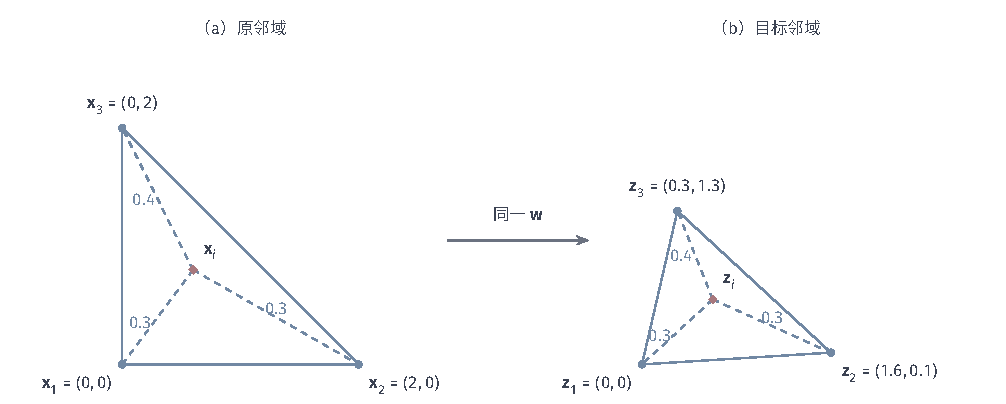
\includegraphics[width=169.000mm]{figures/04-classic-models/00-shared/tikz/dim-lle-weights/figure.pdf}
  \caption{LLE局部权重保持的示意。左图用二维局部坐标绘出三个邻居和菱形中心点；虚线旁为重构权重，其和为1。右图将邻居移至所标位置，同样的权重给出中心$(0.60,0.55)^\top$。两图使用相同的无量纲尺度，实线三角形的形状与边长可以改变。两个画面用于对照高维局部几何与目标邻域，不是完整LLE输出，也不表示一次二维到二维的降维。}
  \label{fig:dim-lle-weights}
\end{figure*}

\subsubsection{参数学习}

按固定顺序排列第$i$个邻域，令$\bm{A}_i\in\mathbb{R}^{q\times d}$的每行为$(\bm{x}_j-\bm{x}_i)^{\top}$，并记$\bm{C}_i=\bm{A}_i\bm{A}_i^{\top}$。该邻域的权重$\bm{w}_i\in\mathbb{R}^q$满足
\[
  \min_{\bm{1}^{\top}\bm{w}_i=1}
    \bm{w}_i^{\top}\bm{C}_i\bm{w}_i.
\]
当$\bm{C}_i$正定时，驻点条件为$\bm{C}_i\bm{w}_i=c\bm{1}$。用权重和为一确定$c$，得到
\begin{equation}
  \label{eq:dim-lle-local}
  \bm{w}_i
  =\frac{\bm{C}_i^{-1}\bm{1}}
         {\bm{1}^{\top}\bm{C}_i^{-1}\bm{1}}.
\end{equation}
求权重时直接解线性方程即可。$q>d$使$\bm{C}_i$必然奇异；即使$q\leq d$，局部样本接近低维切空间也可能造成秩亏或病态。可用$\bm{C}_i+\rho_i\bm{I}_q$改善条件数，例如令$\rho_i$与迹成比例。邻居全部重合时迹为零，需另设正的尺度下限或单独处理。加入正则项也改变了原重构目标。

行和约束给出$\bm{M}\bm{1}=\bm{0}$。在常数方向的正交补中，取最小的$k$个特征方向组成单位列矩阵$\bm{U}_k$，则$\bm{Z}=\sqrt n\,\bm{U}_k$解式\eqref{eq:dim-lle-embedding}。零空间只有常数方向时，才能取最小$k+1$个特征向量后丢掉一个。断连分量的指示向量也属于零空间；对于带符号权重，连通本身仍不足以保证零空间只有一维。

额外零模态会使部分坐标只给各分量分配常数，未表达分量内部的形状。分别嵌入各分量也无法由局部关系确定它们的相对位置、方向和尺度，断连问题仍需额外处理。

局部矩阵构造及求解约需$O(nq^2d+nq^3)$。全局阶段可依次乘$\bm{I}_n-\bm{W}$及其转置，无需显式形成$\bm{M}$；一次矩阵向量乘约为$O(nq)$。部分谱求解还受谱隙、迭代次数和重正交成本影响。邻居数$q$、输出维数$k$与正则尺度都需要选择。

对新点先求局部重构权重，再以$\bm{z}(\bm{x})=\sum_{j\in\mathcal{N}(\bm{x})}w_j(\bm{x})\bm{z}_j$插值。训练坐标固定，这一步未重新求全局谱。邻域不稳定或新点远离训练支持时，插值可能失真。

\subsubsection{理论分析}

\paragraph{表达能力}
固定邻域权重后，LLE要求的是$\bm Z=\bm W\bm Z$，而非点间距离相同。若原数据位于一个$m$维仿射子空间，且每个点的邻居能够仿射重构该点，无正则化的权重可使$\bm X=\bm W\bm X$成立。对数据作中心化和任意线性变换仍保留这个等式；当样本实际张成该空间、$k=m$时，再白化坐标即可同时满足列正交约束，得到零嵌入残差。白化会改变长度与角度，因此零残差本身不表示等距恢复。

一般固定权重未必允许$k$个非平凡的零残差方向。只有$\ker(\bm I_n-\bm W)$在常数方向之外至少还有$k$维，才存在满足本节规范化的零目标表示；否则最小残差为正。光滑流形上的局部仿射关系只能近似成立，后面的Taylor展开说明曲率与权重幅度怎样产生剩余误差。邻域关系也不能确定断连分量之间的位置；对齐或插值不能补回图中未提供的关系。

局部重构关系为何可能在降维后保留，可以用坐标函数的Taylor展开解释。令邻居的局部位移为$\bm{\xi}_j$，对光滑函数$f$有
\[
  \begin{aligned}
    f(\bm{x}_i)-\sum_j\bm{W}_{i,j}f(\bm{x}_j)
    ={}&-\nabla f^{\top}\sum_j\bm{W}_{i,j}\bm{\xi}_j\\
       &+O\left(\sum_j|\bm{W}_{i,j}|
                  \lVert\bm{\xi}_j\rVert_2^2\right).
  \end{aligned}
\]
权重和为一消去常数项，加权位移接近零又使一阶项较小，剩余误差主要来自二阶变化。余项中出现权重绝对值，所以大幅正负抵消可能放大误差。噪声还会改变邻域和局部矩阵，局部近似是否可靠需要另行检查。



\paragraph{收敛性}
每个局部权重问题是带仿射约束的凸二次问题，最小值存在；局部矩阵正定时解唯一，奇异时可能有多个解。加入正的对角正则可以得到唯一权重，但会改变局部重构目标。冻结权重后，$k\leq n-1$时中心化且规范化的坐标集紧致，嵌入最小值存在，并由常数方向正交补中的最小$k$个特征方向达到。截断位置有谱间隔时，最优子空间唯一，坐标仍允许正交旋转。求特征向量的迭代速度依赖谱间隔与求解器；两阶段求解的精确性也不表示它在联合优化权重与坐标。

\paragraph{泛化性}
固定邻域权重后，令$I$在训练索引中均匀抽取，LLE的局部关系风险为
\[
 R_G(\bm Z)=\mathbb E_I\left\lVert\bm z_I
                 -\sum_jW_{I,j}\bm z_j\right\rVert_2^2
            =\frac1n\operatorname{tr}(\bm Z^\top\bm M\bm Z).
\]
在式\eqref{eq:dim-lle-embedding}的约束下，记常数方向正交补中最小的$k$个特征值为$\nu_1,\ldots,\nu_k$。谱解达到
$R_G^\star=\sum_{\ell=1}^k\nu_\ell$；若完整目标的数值误差为$e_G$，则
$R_G(\widehat{\bm Z})\leq\sum_{\ell=1}^k\nu_\ell+e_G/n$。
这个期望只对固定对象集上的随机索引取平均，不能称为独立新点风险。局部插值规定了新点编码，但若未另外规定总体目标坐标函数、采样密度与权重稳定条件，就没有从训练残差到新点重构或几何损失的界。Hessian LLE与LTSA改变局部目标，同样需按各自目标分析，不能套用本节的特征值和。

\subsubsection{优化表达能力}

\paragraph{约束展开坐标的局部曲率}
LLE保留局部的一阶组合关系，还可以进一步约束坐标在局部怎样弯曲。Donoho与Grimes在2003年提出的\term{Hessian LLE}（Hessian特征映射）估计局部坐标函数的二阶变化，寻找其平方积分接近零的方向。这样做的依据是：连通且局部等距于欧氏区域等条件下，展开坐标在局部为仿射函数，Hessian为零。原理论允许某些非凸、带孔参数区域，但未涵盖任意带孔流形；估计二阶项还需足够且分布合适的邻居，采样要求通常比一阶拟合更强\scite{dimDonoho2003}。在$m$维展开区域对应的连续理想模型中，常数与$m$个展开坐标张成$m+1$维零空间，排除常数后即可恢复展开表示；有内在曲率的流形未必具有这些零Hessian坐标，有限样本中估计到的小特征值也还包含邻域和求谱误差。

\paragraph{协调邻域之间的坐标方向}
弯曲点集的各小块可以分别近似为平面，但不同小块的平面朝向不同，局部PCA坐标不能直接拼在一起。Zhang与Zha在2004年的\term{局部切空间对齐}（local tangent space alignment, LTSA）中，在邻域内估计$m$维切空间及局部坐标，再寻找一组全局坐标，使它们经过各邻域的仿射变换后与局部坐标对齐。重叠邻域提供了拼接所需的共同样本，切空间估计与邻域选择的误差也会传到全局\scite{dimZhang2004}。若目标全局坐标与每块局部坐标之间确实有一致的仿射关系，候选对齐就能做到零残差；若局部弯曲在所选尺度下不可忽略，仿射变换只能近似它。重叠不足时，各块的位置还可分别改变，局部精确并不唯一确定整体表示。

\subsubsection{小结}

LLE保留样本与邻居之间的仿射重构关系，再让这些局部关系共同约束坐标。邻域尺度和局部秩影响权重，权重是否稳定也影响不同小块怎样拼接；局部残差小不能单独说明整体几何已经保留。

Hessian LLE进一步使用局部二阶变化，回应展开坐标应怎样弯曲的问题，同时需要更充分的局部采样。LTSA改为估计并对齐邻域切空间，让重叠样本连接各块坐标，同时增加局部方向估计及对齐误差。两者改变了局部目标，选择时应检查数据支持的是仿射重构、局部等距展开还是切空间拼接。

\subsection{拉普拉斯特征映射（Laplacian Eigenmaps）}
\label{sec:dim-le}

局部信息也可以只说明“这两个样本应当靠近”，而不要求给出路径长度或重构权重。例如，相邻时刻的观测若变化平缓，我们希望它们的低维坐标也平缓变化。\term{拉普拉斯特征映射}（Laplacian Eigenmaps）给相似点连边，对边两端的坐标差施加平方惩罚；边权越大，分开这两个点的代价越大。若只有这项惩罚，把全部点放在同一处就会得到零值，所以还需中心化与尺度约束防止塌缩。Belkin与Niyogi在NIPS 2001介绍相关谱方法，2003年期刊论文展开其模型与几何联系\scite{dimBelkin2003}它与第\ref{sec:clustering-spectral}节的谱聚类共享图拉普拉斯与低频特征方向，直接输出连续坐标，谱聚类则继续将这些坐标转为簇分配。

\subsubsection{模型结构}

在对称邻域图上设非负权重$\bm{W}_{i,j}$。相邻点可取$\exp(-\lVert\bm{x}_i-\bm{x}_j\rVert_2^2/(4\tau))$或$1$，其他位置为零，$\tau>0$控制衰减尺度。令$b_i=\sum_j\bm{W}_{i,j}$、$\bm{D}_b=\operatorname{diag}(b_1,\ldots,b_n)$，图拉普拉斯为$\bm{L}=\bm{D}_b-\bm{W}$。对标量信号$\bm{f}\in\mathbb{R}^n$，由对称性有
\begin{equation}
  \label{eq:dim-le-energy}
  \bm{f}^{\top}\bm{L}\bm{f}
  =\frac12\sum_{i,j}\bm{W}_{i,j}(f_i-f_j)^2.
\end{equation}
能量非负，故$\bm{L}$半正定，常数信号的能量为零。将各坐标列的能量相加，得到
\begin{equation}
  \label{eq:dim-le-objective}
  \begin{aligned}
    \min_{\bm{Z}}\quad&
      \operatorname{tr}(\bm{Z}^{\top}\bm{L}\bm{Z}),\\
    \text{满足}\quad&
      \bm{Z}^{\top}\bm{D}_b\bm{Z}=\bm{I}_k,\qquad
      \bm{Z}^{\top}\bm{D}_b\bm{1}=\bm{0}.
  \end{aligned}
\end{equation}
度加权范数排除零解，加权中心化排除常数方向。缺少后一个约束，就可能将没有区分能力的常数列纳入嵌入。目标只惩罚邻近点的坐标差异，远点是否分开还由全局约束和所选模式决定。

\subsubsection{参数学习}

对坐标列求驻点，在常数的加权正交补中得到$\bm{L}\bm{v}=\lambda\bm{D}_b\bm{v}$。各点度为正时，令$\bm{u}=\bm{D}_b^{1/2}\bm{v}$，将它化成对称特征值问题：
\[
  \bm{L}_{\mathrm{sym}}\bm{u}=\lambda\bm{u},
  \qquad
  \bm{L}_{\mathrm{sym}}
  =\bm{I}_n-\bm{D}_b^{-1/2}\bm{W}\bm{D}_b^{-1/2}.
\]
求得单位向量后，要变回$\bm{v}=\bm{D}_b^{-1/2}\bm{u}$以满足模型的归一化。连通图的广义问题以常数为零特征向量，对称问题的零方向却与$\bm{D}_b^{1/2}\bm{1}$成比例。多个连通分量对应多个零模态，应一并识别；零度点也需单独处理，不能直接作逆度归一化。

若权重矩阵有$O(nq)$个非零元，一次矩阵向量乘为$O(nq)$。总求解成本还包括建图、$k$个方向的迭代及正交化。$q$控制哪些点连接，$\tau$控制连接强弱，$k$控制保留的模式数。过小带宽可能使部分度数接近零，过大带宽则削弱局部差异，可结合图诊断与任务表现选择。

\subsubsection{理论分析}
\label{sec:dim-le-theory}

\paragraph{表达能力}
拉普拉斯坐标能够表示的是选定图上的低频变化。设图连通且各点度为正，把广义特征向量按$\bm D_b$内积归一化，以$\bm v_0$表示常数方向、$\bm v_1,\ldots,\bm v_{n-1}$表示非平凡方向。任何节点信号都可展开为$\bm f=\sum_{\ell=0}^{n-1}a_\ell\bm v_\ell$；若信号只使用前$k$个非平凡模式及常数，它就能由这组表示精确线性重构。舍弃其他模式后的度加权平方误差为$\sum_{\ell>k}a_\ell^2$，依据正是特征方向的加权正交性。

较大的广义特征值对应跨强边变化较快的模式，因而快速切换的标签或局部突变可能在低频截断时丢失。在连通图上，零能量又要求每条正权边的两个端点坐标相同，最终使全部节点重合；本节的非塌缩约束排除了它，所以一个有区分能力的嵌入必须保留正能量。小能量只是图上平滑，没有约束原距离或角度，也不保证不同节点必有不同坐标。

\paragraph{收敛性}
固定非负邻域图后，广义特征值问题给出约束能量的全局最优解。截断处有谱隙时，所选子空间唯一。迭代速度取决于谱隙、预条件和残差要求；有限图上的数值收敛与采样图逼近流形属于不同问题。

\paragraph{泛化性}
拉普拉斯特征映射的原始学习器也只输出训练节点坐标。固定非负对称图，令$S_w=\sum_{i,j}w_{ij}>0$，按$w_{ij}/S_w$抽取有序节点对$(I,J)$，则
\[
 R_G(\bm Z)=\mathbb E\lVert\bm z_I-\bm z_J\rVert_2^2
          =2\operatorname{tr}(\bm Z^\top\bm L\bm Z)/S_w.
\]
在本节的度归一化与常数方向排除约束下，设最小的$k$个可用广义特征值为$\nu_1,\ldots,\nu_k$，谱解的风险为
$R_G^\star=2\sum_{\ell=1}^k\nu_\ell/S_w$。
若迹目标求解误差为$e_G$，则
$R_G(\widehat{\bm Z})\leq R_G^\star+2e_G/S_w$。
这是给定图上的期望邻接损失，未评价独立新点。要把它扩展为总体函数的风险，还须规定延拓、连续能量和采样条件；下面的谱一致性结论解释离散与连续对象的联系，但本身没有给出有限样本的新点损失界。

讨论新样本时，需要将离散能量与连续几何联系起来。式\eqref{eq:dim-le-energy}对应的\term{Dirichlet能量}积分了函数沿流形的变化率平方。采用非负号约定$\Delta_{\mathcal{M}}=-\operatorname{div}_{\mathcal{M}}\nabla_{\mathcal{M}}$，在紧致无边界流形上有
\begin{equation}
  \label{eq:dim-dirichlet}
  \mathcal{E}(f)
  =\int_{\mathcal{M}}\lVert\nabla_{\mathcal{M}}f\rVert_2^2\,\mathrm{d}V
  =\int_{\mathcal{M}}f\Delta_{\mathcal{M}}f\,\mathrm{d}V.
\end{equation}
Laplace--Beltrami算子描述函数沿流形的局部变化，对应欧氏空间的负拉普拉斯。求均值为零、平方积分为一的最平滑函数时，给能量加入约束乘子，并沿光滑扰动$g$求导：
\[
  2\int_{\mathcal{M}}g\Delta_{\mathcal{M}}f\,\mathrm{d}V
  -2\lambda\int_{\mathcal{M}}gf\,\mathrm{d}V
  -2c\int_{\mathcal{M}}g\,\mathrm{d}V=0.
\]
分部积分产生第一项。取$g=1$得到$c=0$，再由扰动任意得到$\Delta_{\mathcal{M}}f=\lambda f$。逐次加入与已有特征函数正交的约束，就按频率从低到高得到函数方向。这一变分关系解释了低频坐标的平滑性。

图与流形之间要分别考察算子和谱。点态收敛作用于固定光滑函数，谱收敛则比较随样本改变的特征值与特征函数，前者不能直接推出后者。Belkin与Niyogi在2006年的谱收敛研究中，分别处理经验算子的谱逼近及小带宽下的连续谱逼近\scite{dimBelkin2006}

\begin{lemma}[一种定性的谱一致性结论]
  \label{thm:dim-le-spectral}
  设$\mathcal{M}$是紧致、连通、无边界的$C^\infty$嵌入$m$维黎曼流形，为简化常数令其体积为一。样本独立均匀采自$\mathcal{M}$。考虑全连接高斯图对应的经验算子
  \[
    \begin{aligned}
      \widehat{\mathcal{L}}_{n,\tau}f(\bm{x})
      ={}&\frac{1}{n\tau(4\pi\tau)^{m/2}}\\
      &\cdot\sum_{j=1}^n
        e^{-\lVert\bm{x}-\bm{x}_j\rVert_2^2/(4\tau)}
        \bigl(f(\bm{x})-f(\bm{x}_j)\bigr).
    \end{aligned}
  \]
  存在趋于零而足够缓慢的带宽序列$\tau_n$，使每个固定的低频特征值依概率收敛到$\Delta_{\mathcal{M}}$的相应特征值。将经验特征向量按该算子延拓并作$L^2(\mathcal{M})$归一化后，孤立单特征值对应的特征函数可在符号对齐后依概率收敛；重特征值应按相应有限维特征子空间比较。
\end{lemma}

该结论针对给定的全连接高斯算子，只断言存在合适带宽序列。归一化幂次用内在维数$m$，且算子未作度归一化。它与模型的广义特征值问题之间还需尺度校正：均匀采样下，度的极限趋向空间常数，可以联系两者；非均匀采样、稀疏截断或流形有边界时，要重新分析度、极限测度及边界条件。

非均匀密度$p$下，未修正的局部能量一般带$p^2$权重，密集区域因而更影响低频表示。谱收敛也未保证少量特征函数组成的映射单射或保留全部距离。新点可用核特征函数延拓，或另学映射。标签传播在给定类别语义下求得分，谱聚类输出簇，本节输出坐标；它们共享图平滑，但目标与评价不同（参见第\ref{sec:classification-label-propagation}、\ref{sec:clustering-spectral}节）。

\subsubsection{小结}

拉普拉斯特征映射用图上的平滑变化组织坐标。邻域权重与归一化决定比较关系，求解时还需处理断连和零模态；坐标适合哪些用途，应回到所建图与原始数据检查。

\subsection{扩散映射（Diffusion Map）}
\label{sec:dim-diffusion}

单条边只记录一对点的关系，更多步的连接还可以描述它们处于怎样的邻域环境。设想在相似度图上随机行走：两点即使没有直接连边，若从它们出发都容易到达同一片区域，也可以被视为接近。\term{扩散映射}（diffusion map）比较两个起点经过相同步数后的到达分布，再把这种分布差异写为低维坐标的距离。较小步数侧重局部连接，较大步数把更多路径纳入比较，也可能抹平局部差异。Coifman与Lafon在2006年建立了这一扩散距离的谱表示，并用时间参数选择尺度\scite{dimCoifman2006}它与拉普拉斯特征映射共享谱计算，但对坐标缩放与点间距离给出了随机行走的含义。

\subsubsection{模型结构}

以对称非负矩阵$\bm{K}$表示原始相似度，可用全连接高斯核或稀疏邻域权重。记原始度为$r_i$，密度重加权后的度为$b_i$，以避免与邻居数$q$混淆。归一化过程为
\begin{equation}
  \label{eq:dim-diffusion-normalization}
  \begin{aligned}
    r_i&=\sum_j\bm{K}_{i,j},&
    \widetilde{\bm{K}}_{i,j}
      &=\frac{\bm{K}_{i,j}}{r_i^\alpha r_j^\alpha},\\
    b_i&=\sum_j\widetilde{\bm{K}}_{i,j},&
    \bm{P}_{i,j}&=\frac{\widetilde{\bm{K}}_{i,j}}{b_i},
    \qquad 0\leq\alpha\leq1.
  \end{aligned}
\end{equation}
假设度数均为正。$\bm{P}$每行和为一，其元素表示一步转移概率。重加权后的度确定平稳分布：
\begin{equation}
  \label{eq:dim-diffusion-stationary}
  \pi_i=\frac{b_i}{\sum_j b_j},
  \qquad
  \pi_i\bm{P}_{i,j}=\pi_j\bm{P}_{j,i}.
\end{equation}
末式是细致平衡关系，故$\bm{\pi}^{\top}\bm{P}=\bm{\pi}^{\top}$。按行写分布与列向量方程$\bm P^\top\bm\pi=\bm\pi$等价（参见\BookSectionRef{sec:rv-markov}{卷2《数学准备：概率、因果与决策》第1章“随机变量”第1.2.5节“历史条件下的状态依赖”}）。平稳分布使用$b_i$；只有$\alpha=0$等特殊情形，才可由原始$r_i$直接计算。

对整数$t\geq0$，以$p_t(i,j)=(\bm{P}^t)_{i,j}$表示$t$步转移概率。定义扩散距离
\begin{equation}
  \label{eq:dim-diffusion-distance}
  D_t^2(i,j)
  =\sum_{a=1}^n\frac{(p_t(i,a)-p_t(j,a))^2}{\pi_a}.
\end{equation}
距离比较整个到达分布，各目标点的差异按平稳概率校正；很少被访问的点上，同样的概率差会计入更大贡献。若两个起点有相同到达分布，距离也会为零，故一般可为伪度量。跨区域瓶颈减缓混合，使部分时间尺度仍能区分这些区域。

图\ref{fig:dim-diffusion-walk}中，两个团只由一条弱边相连。团内传播快，跨团传播慢，4步后大部分概率仍在起点一侧；64步时两行分布已更接近，仍未相同。扩散距离比较这些概率差，节点在示意图中的间隔不参与计算。

\begin{figure}[htbp]
  \centering
  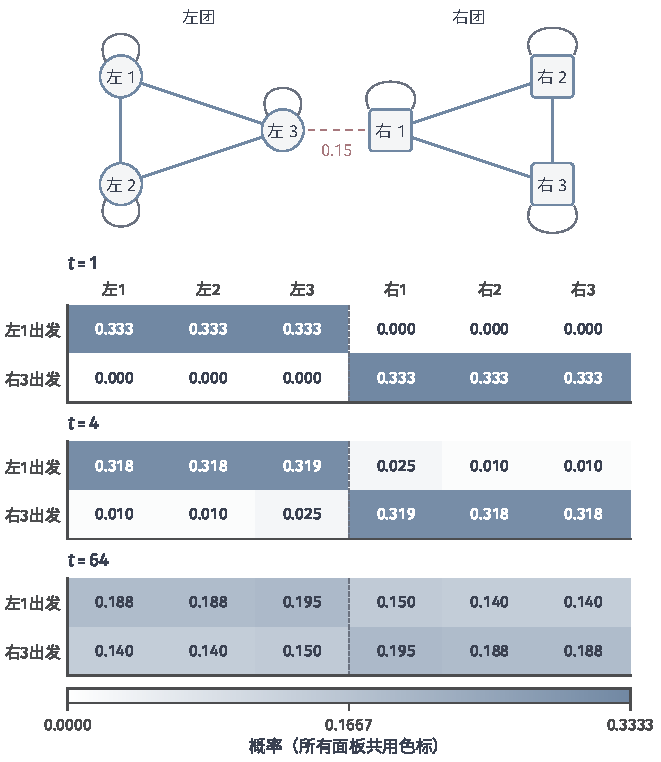
\includegraphics[width=105.412mm]{figures/04-classic-models/00-shared/matplotlib/dim-diffusion-walk/figure.pdf}
  \caption{扩散时间与跨团瓶颈。每团三个节点，团内边及所有自环权重为1，唯一跨团边权重为$0.15$。令$\alpha=0$并按行归一化，热图两行分别表示从左1、右3出发的$\bm{P}^t$对应行，六列为固定节点顺序；各时刻共用同一连续概率色标。数值由有理数矩阵乘法计算，显示三位小数，舍入后行和可能略偏离1。64步仍未充分混合；因图连通且有自环，极限分布均为$\bm{\pi}^{\top}=(20,20,21,21,20,20)/122$。}
  \label{fig:dim-diffusion-walk}
\end{figure}

\subsubsection{参数学习}

记$\bm{\Pi}=\operatorname{diag}(\pi_1,\ldots,\pi_n)$。由细致平衡，矩阵
\[
  \bm{S}=\bm{\Pi}^{1/2}\bm{P}\bm{\Pi}^{-1/2}
\]
为对称矩阵。取其欧氏单位特征向量$\bm{u}_\ell$，并令$\bm{\psi}_\ell=\bm{\Pi}^{-1/2}\bm{u}_\ell$，则
\begin{equation}
  \label{eq:dim-diffusion-eigenvectors}
  \begin{aligned}
    \bm{P}\bm{\psi}_\ell&=\lambda_\ell\bm{\psi}_\ell,\\
    \sum_i\pi_i\psi_\ell(i)\psi_r(i)&=\delta_{\ell,r}.
  \end{aligned}
\end{equation}
这些特征函数在$L^2(\bm{\pi})$内积下正交。连通图的常数特征对为$\lambda_0=1,\psi_0(i)=1$，其余特征值在$[-1,1]$内。再满足非周期性时，非平凡特征值的绝对值小于一。连通图保留正自环即可保证非周期性，无自环二部图却可能出现$-1$特征值。

非负对称权重仍可能有负特征值，应按$|\lambda_1|\geq|\lambda_2|\geq\cdots$选择扩散模态。全连接半正定核经对角缩放仍半正定，此时才可按非负特征值降序选取；稀疏截断可能破坏半正定性。$k$维扩散坐标定义为
\begin{equation}
  \label{eq:dim-diffusion-map}
  \bm{\Psi}_{t,k}(i)
  =\bigl(\lambda_1^t\psi_1(i),\ldots,
         \lambda_k^t\psi_k(i)\bigr)^{\top}.
\end{equation}
将这些坐标按行放置，得到$n\times k$矩阵。$t$对应转移矩阵的整数幂；含负特征值时，直接令$t$取任意实数将失去这一解释。

稠密矩阵的构造、存储及完整谱分解成本与核PCA同阶。稀疏权重降低矩阵向量乘成本，总求谱时间仍受$k$、谱间隔及精度影响。除邻域或带宽与$k$外，还要选择$\alpha$和$t$；同一组谱可在不同$t$下重新加权，无需重复分解。

\subsubsection{理论分析}
\label{sec:dim-diffusion-theory}

\paragraph{表达能力}
扩散映射要表达的是两个起点经过$t$步后到达分布的差异。若两个起点的到达分布相同，扩散距离就是零，表示会将它们视为同一状态，即使原空间中两点相距很远。对给定可逆转移矩阵，保留全部非平凡模态能够精确实现这一距离；保留$k$个模态后的平方失真，是未保留模态的非负贡献之和。下面的定理给出该和及上界，因此可以据谱尾部判断指定维数对这一目标是否足够。

扩散时间改变目标本身。只有需要区分的到达分布差异主要由所保留的慢模态承担，低维截断才会近似保留这些差异；若重要差异来自快速模态，增大$t$反而会把它们抹去。核、密度重加权和步数还改变转移过程，所以精确表达扩散距离并不意味着精确表达欧氏距离或测地距离。

下面在$L^2(\bm{\pi})$中展开转移概率，用正交性消去交叉项，得到有限图上的精确关系与截断界。核尺度与采样图的结构误差仍需另行检查。

\begin{theorem}[扩散映射对固定图扩散距离的表示误差界]
  \label{thm:dim-diffusion-isometry}
  设$\bm{P}$由连通的对称非负权重构造，$\pi_i>0$，特征函数按式\eqref{eq:dim-diffusion-eigenvectors}归一化。对整数$t\geq0$，全部非平凡模态给出
  \begin{equation}
    \label{eq:dim-diffusion-identity}
    D_t^2(i,j)
    =\sum_{\ell=1}^{n-1}\lambda_\ell^{2t}
      \bigl(\psi_\ell(i)-\psi_\ell(j)\bigr)^2.
  \end{equation}
  当$t=0$时按$\bm{P}^0=\bm{I}_n$约定所有模态系数为一。若按特征值绝对值排序，$k<n-1$且$i\ne j$，截断的平方距离误差$R_{t,k}$满足
  \begin{equation}
    \label{eq:dim-diffusion-tail}
    \begin{aligned}
      R_{t,k}(i,j)
        &:=D_t^2(i,j)
          -\lVert\bm{\Psi}_{t,k}(i)-\bm{\Psi}_{t,k}(j)\rVert_2^2,\\
      0\leq R_{t,k}(i,j)
        &\leq|\lambda_{k+1}|^{2t}
          \left(\frac1{\pi_i}+\frac1{\pi_j}\right).
    \end{aligned}
  \end{equation}
\end{theorem}
\begin{proof}
  对称矩阵$\bm{S}$的谱分解给出
  \[
    p_t(i,a)=\pi_a\sum_{\ell=0}^{n-1}
      \lambda_\ell^t\psi_\ell(i)\psi_\ell(a).
  \]
  令$c_\ell=\lambda_\ell^t(\psi_\ell(i)-\psi_\ell(j))$，则$c_0=0$。代入定义，展开平方并使用加权正交性：
  \[
    \begin{aligned}
      D_t^2(i,j)
        &=\sum_a\pi_a
          \left(\sum_{\ell=1}^{n-1}c_\ell\psi_\ell(a)\right)^2\\
        &=\sum_{\ell,r=1}^{n-1}c_\ell c_r
          \sum_a\pi_a\psi_\ell(a)\psi_r(a)
         =\sum_{\ell=1}^{n-1}c_\ell^2.
    \end{aligned}
  \]
  其中$\pi_a$来自分子中$\pi_a^2$除以定义中的$\pi_a$，不能再次消去。截断后余项是$\ell>k$的非负和。由绝对值排序及完整正交基关系，
  \[
    \begin{aligned}
      R_{t,k}
        &\leq|\lambda_{k+1}|^{2t}
          \sum_{\ell=1}^{n-1}
            (\psi_\ell(i)-\psi_\ell(j))^2,\\
      \sum_{\ell=0}^{n-1}\psi_\ell(i)\psi_\ell(j)
        &=\frac{\delta_{i,j}}{\sqrt{\pi_i\pi_j}},
    \end{aligned}
  \]
  对$i\ne j$展开平方，即得所述上界；$i=j$时两种距离和余项都为零。
\end{proof}

保留全部$n-1$个模态时距离精确，截取$k$维则一般有误差。式\eqref{eq:dim-diffusion-tail}同时含谱尾部与平稳概率，稀少区域可能有更大的绝对误差界。增大时间虽使该界缩小，真实扩散距离也随之缩小，不能据此保证相对精度改善。

不可约且非周期的有限链满足$|\lambda_\ell|<1$，故$t\to\infty$时，各起点的到达分布趋于$\bm{\pi}^{\top}$，距离也趋于零。混合前的较大$t$突出慢模态，过大的$t$则丢失区分。连续时间可另用$\exp[-s(\bm{I}_n-\bm{P})]$，以$e^{-s(1-\lambda_\ell)}$加权。

使用同一组对称权重时，拉普拉斯广义问题与转移矩阵满足
\[
  (\bm{D}_b-\bm{W})\bm{v}=\mu\bm{D}_b\bm{v}
  \quad\Longleftrightarrow\quad
  \bm{P}\bm{v}=(1-\mu)\bm{v}.
\]
两者因而共享特征方向。将选定模态的时间权重设为一，并调整归一化，可得到无时间加权的拉普拉斯坐标；$L^2(\bm{\pi})$与$\bm{D}_b$的归一化还差全局尺度。负谱存在时，按绝对值排序的扩散映射可能选中拉普拉斯高端模态，这一选择也需计入比较。

\paragraph{收敛性}
固定满足细致平衡的转移矩阵后，扩散坐标由谱分解求得。残差决定数值精度，谱分离和求解器影响迭代速度。游走时间$t$选择表示尺度，与求谱算法的迭代次数分别控制不同问题。

\paragraph{泛化性}
扩散映射有一个无需总体采样假设的有限图风险结论。固定转移矩阵及$t$，让$I,J$独立按平稳分布$\bm\pi$抽取，用未保留的平方扩散距离作为损失。由定理\ref{thm:dim-diffusion-isometry}及非平凡特征函数的零均值、单位$L^2(\bm\pi)$范数，得到
\begin{equation}
 \mathbb E_{I,J\sim\bm\pi}R_{t,k}(I,J)
 =2\sum_{\ell=k+1}^{n-1}\lambda_\ell^{2t}
 \leq2(n-1-k)|\lambda_{k+1}|^{2t}.
 \label{eq:dim-diffusion-graph-risk}
\end{equation}
每个舍弃模态的两点差平方期望为$2$，所以此处给出精确的平均截断损失，而非仅用最小平稳概率放大的逐点上界。风险仍只对固定图中的节点抽取，未涉及独立新对象；Nystr\"om延拓定义编码以后，还需控制经验转移算子与总体转移算子的误差，才能得到相应总体扩散风险。


密度修正要在采样极限中解释。在光滑正密度$p$、足够采样及小高斯带宽的内点极限下，生成元含有与$2(1-\alpha)\nabla_{\mathcal{M}}\log p$有关的漂移。$\alpha=1$消去主导密度漂移，使极限扩散由流形几何决定；有限样本仍可能有密度影响。$\alpha=0$保留密度作用，适用于任务本身关注该概率结构的情形。

新点可用Nystr\"om方式延拓。沿用训练核及$r_j$，计算$r(\bm{x})=\sum_j\kappa(\bm{x},\bm{x}_j)$，按训练归一化构造$p(\bm{x},j)$。当$\lambda_\ell\ne0$时，有
\begin{equation}
  \label{eq:dim-diffusion-extension}
  \psi_\ell(\bm{x})
  =\frac1{\lambda_\ell}\sum_jp(\bm{x},j)\psi_\ell(j),
  \qquad
  z_\ell(\bm{x})=\lambda_\ell^t\psi_\ell(\bm{x}).
\end{equation}
该式固定训练度和谱，将特征方程延伸到新点。小特征值的倒数会放大误差，零特征值需其他处理。错误连接对传播的影响取决于它如何改变瓶颈，使用多条路径也不能保证减弱每一条错误边的作用。

\subsubsection{优化表达能力}

\paragraph{纳入局部方向关系}

普通扩散映射比较走到哪里的概率，没有同时说明沿路径怎样保持方向。若任务还关心局部切方向在不同区域之间是否一致，就可以把邻域切空间的对齐关系放入传播。Singer与Wu的\term{向量扩散映射}（vector diffusion maps）用正交对齐矩阵记录这些关系，使路径上的方向运输参与比较\scite{dimSinger2012}。其连续对象是作用于向量场的连接拉普拉斯。由这些方向传播关系形成的距离和嵌入，可以区分仅靠标量到达概率没有刻画的局部方向关系；输出仍可采用嵌入坐标，所改进的是表示中保留的信息。

\subsubsection{小结}

扩散映射用多步传播比较样本的到达分布，适合关系需要通过多条局部路径累积的情形。核尺度决定局部联系，重加权调整采样密度的作用，传播时间选择观察粒度；时间过长还可能混合原本要区分的区域，新点延拓则需要沿用训练归一化。

向量扩散映射把切空间对齐加入传播，扩展了嵌入可以利用的几何关系。若研究对象转为图或流形上的函数，Coifman与Maggioni的扩散小波还可用扩散算子的幂构造多尺度函数基，服务于函数近似与算子压缩\scite{dimCoifmanMaggioni2006}。这已经超出本节以低维坐标表示样本的任务，函数基的压缩和正交化需要另作分析。

\subsection{随机邻居嵌入（SNE）}
\label{sec:dim-sne}

同一个距离阈值在稠密区域可能包含许多点，在稀疏区域却只包含一两个点。如果目的是显示每个样本最相关的邻居，就可以先比较它与其他点的相对接近程度，而不要求所有原始距离都按同一比例缩小。Hinton与Roweis于2002年提出\term{随机邻居嵌入}（stochastic neighbor embedding，SNE），为每个样本建立选择邻居的概率分布，再调整低维位置，尽量复现这些概率。局部带宽控制一行分布中的有效邻居数量，使不同疏密区域可以采用不同距离尺度。“随机”指邻居选择的概率模型，坐标仍由优化求得。

原论文用bank的歧义说明表示的局限：河岸与金融是不同语境，单一位置可能难以同时容纳两组邻居。因此作者也讨论了同一对象具有多个位置的混合扩展\scite{dim-hinton2002sne}本节采用单位置形式；邻域分布定义之后，还需判断低维空间能否表达这些关系。

\subsubsection{模型结构}

以$i$为中心，用高斯核将距离转为选择邻居的条件概率：
\begin{equation}
  \label{eq:dim-sne-high}
  \begin{aligned}
    p_{j\mid i}
      &=\frac{\exp(-\delta_{i,j}^2/(2\sigma_i^2))}
      {\sum_{\ell\ne i}\exp(-\delta_{i,\ell}^2/(2\sigma_i^2))},
      \qquad j\ne i,\\
    p_{i\mid i}&=0,\qquad \sum_{j\ne i}p_{j\mid i}=1.
  \end{aligned}
\end{equation}
带宽$\sigma_i>0$决定局部尺度。小带宽将概率集中到近邻，大带宽使远点获得更多权重。两点距离虽对称，条件概率通常不对称，因为各中心的带宽及归一化分母不同。

\term{困惑度}（perplexity）将分布$P_i=(p_{j\mid i})_{j\ne i}$的熵转为有效邻居数，以此校准带宽。采用自然对数时定义
\begin{equation}
  \label{eq:dim-sne-perplexity}
  \begin{aligned}
    H(P_i)&=-\sum_{j\ne i}p_{j\mid i}\log p_{j\mid i},\\
    \operatorname{Perp}(P_i)&=\exp\!\bigl(H(P_i)\bigr).
  \end{aligned}
\end{equation}
概率在$q$个邻居上均匀分配时，困惑度为$q$。一般值可以非整数，未规定固定数量的非零邻居。熵若改用以$2$为底的对数，外层应改为$2^{H_2(P_i)}$。

带宽可根据目标困惑度$\tau$二分搜索。记$\beta_i=1/(2\sigma_i^2)$、$D_j=\delta_{i,j}^2$及$B_i=\sum_{j\ne i}\exp(-\beta_iD_j)$，则
\begin{equation}
  \label{eq:dim-sne-entropy-monotonicity}
  \begin{aligned}
    H(P_i)&=\log B_i+\beta_i\mathbb{E}_{P_i}[D],\\
    \frac{\mathrm{d}}{\mathrm{d}\beta_i}\mathbb{E}_{P_i}[D]
      &=-\operatorname{Var}_{P_i}(D),\\
    \frac{\mathrm{d}H(P_i)}{\mathrm{d}\beta_i}
      &=-\beta_i\operatorname{Var}_{P_i}(D)\leq 0.
  \end{aligned}
\end{equation}
困惑度随带宽单调不减；距离不全相等时严格递增。设并列最近邻有$h_i$个，带宽从零趋向无穷时，困惑度从$h_i$趋向$n-1$，故$\tau\in(h_i,n-1)$才对应唯一有限正带宽。所有距离相等时值恒为$n-1$，重复或并列距离也会限制可达目标。

达到相同困惑度时，稀疏区域通常需更大带宽，稠密区域需更小带宽，所以校准后的邻域分布未直接保留原始密度。可从$5$至$50$探索困惑度，并结合样本数与群体规模调整。预处理仍重要：无关特征改变输入距离后，带宽搜索也会使用这些距离。

低维核尺度固定，坐标通过以下目标学习：
\begin{equation}
  \label{eq:dim-sne-low-loss}
  \begin{aligned}
    q_{j\mid i}
      &=\frac{\exp(-r_{i,j}^2)}
      {\sum_{\ell\ne i}\exp(-r_{i,\ell}^2)},\qquad q_{i\mid i}=0,\\
    C_{\mathrm{SNE}}(\bm{Z})
      &=\sum_i\operatorname{KL}(P_i\Vert Q_i)\\
      &=\sum_i\sum_{j\ne i}p_{j\mid i}
        \log\frac{p_{j\mid i}}{q_{j\mid i}}.
  \end{aligned}
\end{equation}
这里$Q_i=(q_{j\mid i})_{j\ne i}$。核$\exp(-r^2)$与方差为$1/2$、标准差为$1/\sqrt{2}$的高斯密度具有相同形状；固定带宽也就规定坐标单位。共同带宽的改变可由坐标缩放吸收，但在固定带宽下缩放坐标会改变概率与目标。

较大的$p_{j\mid i}$使近邻错置受到较大惩罚：拉远这对点会增加$-\log q_{j\mid i}$。高维远点若挤在低维近处，也会占用归一化概率，减少真正近邻的份额，因而产生排斥作用。整体KL散度非负，单个求和项仍可为负。

\subsubsection{参数学习}

先由$\bm{X}$和$\tau$求带宽并固定$P_i$，再优化坐标。令$A_i=\sum_{\ell\ne i}\exp(-r_{i,\ell}^2)$，以$i$为中心的散度展开为
\begin{equation}
  \label{eq:dim-sne-anchor-loss}
  \begin{aligned}
    C_i&=\sum_{j\ne i}p_{j\mid i}\log p_{j\mid i}
      +\sum_{j\ne i}p_{j\mid i}r_{i,j}^2+\log A_i.
  \end{aligned}
\end{equation}
第一项为常数，第二项按邻居概率拉近点对，第三项反映归一化竞争。求导时必须同时包含后两项，才能得到吸引与排斥共同作用的更新。

$\bm{z}_i$既是$C_i$的中心，也是其他$C_j$的候选邻居。两种贡献分别为
\begin{equation}
  \label{eq:dim-sne-two-roles}
  \begin{aligned}
    \nabla_{\bm{z}_i}C_i
      &=2\sum_{j\ne i}(p_{j\mid i}-q_{j\mid i})
        (\bm{z}_i-\bm{z}_j),\\
    \nabla_{\bm{z}_i}C_j
      &=2(p_{i\mid j}-q_{i\mid j})
        (\bm{z}_i-\bm{z}_j),\qquad j\ne i.
  \end{aligned}
\end{equation}
两个负项分别来自$\log A_i$与$\log A_j$的导数；后者只有含$i$的核项随$\bm{z}_i$变化。将中心与邻居两种贡献相加，得到
\begin{equation}
  \label{eq:dim-sne-gradient}
  \begin{aligned}
    \nabla_{\bm{z}_i}C_{\mathrm{SNE}}
      &=2\sum_{j\ne i}
        \bigl[(p_{j\mid i}-q_{j\mid i})\\
      &\qquad +(p_{i\mid j}-q_{i\mid j})\bigr]
        (\bm{z}_i-\bm{z}_j).
  \end{aligned}
\end{equation}
系数为正时，负梯度更新将$i$拉向$j$；系数为负时将两点推开。因此力的方向由负梯度确定，且需合计两个有向残差，它们可能相互抵消。

用正学习率$\eta_t$作更新$\bm{Z}^{(t+1)}=\bm{Z}^{(t)}-\eta_t\nabla C_{\mathrm{SNE}}(\bm{Z}^{(t)})$，也可加入动量。原工作使用逐渐减弱的随机扰动改善布局，但未保证全局最优。小随机点云能打破全部坐标重合时的对称零梯度状态。

计算完整高维距离需$O(n^2d)$时间，保存概率需$O(n^2)$空间。输出维数固定时，每轮优化为$O(n^2)$。可结合目标值、梯度或位移判断数值进展，再检查近邻保留；数值停止变化只说明当前优化状态。

\subsubsection{理论分析}
\label{sec:dim-sne-theory}

\paragraph{表达能力}
SNE能否精确匹配邻域关系，要看目标条件概率能否由同一组$k$维欧氏距离产生。目标值为零当且仅当每行$Q_i=P_i$。由式\eqref{eq:dim-sne-low-loss}取对数，精确匹配要求存在每行的常数$c_i$，使
\[
 r_{i,j}^2=-\log p_{j\mid i}+c_i\qquad(i\ne j),
\]
且这些数同时构成一个$k$维欧氏平方距离矩阵。它们必须非负、对称，并满足经典MDS的半正定与秩条件；只为每行单独安排邻居，不能保证这些条件同时成立。若高维条件概率原本由某个$k$维点集及统一带宽产生，坐标缩放便可精确匹配；逐点带宽不同或目标维数不足时，则可能留下正的KL误差。

概率目标强调邻域份额，未要求恢复原始距离或采样密度。改变各点带宽已经改变距离到概率的换算，因此即使概率匹配很好，也不能将簇间间距直接读作原空间间距。

\term{拥挤问题}（crowding problem）来自高维邻域与低维空间容量的差异。局部均匀采样于$m$维流形、尺度足够小且远离边界时，半径$r$内样本数近似随$r^m$增长，$k$维体积则随$r^k$增长。这里用的是内在维数$m$；这一比较提供直觉，实际计数还依赖数据与尺度。

$m>k$时，许多中距离关系可能争夺有限位置，高斯核快速衰减进一步限制布局。图\ref{fig:dim-neighbor-tails}中，$r=3$时高斯核约为$0.00012$，Cauchy形核为$0.1$，后者在较远位置仍保留相似度。图中是核值，归一化后的概率还取决于其他点。

\begin{figure}[htbp]
  \centering
  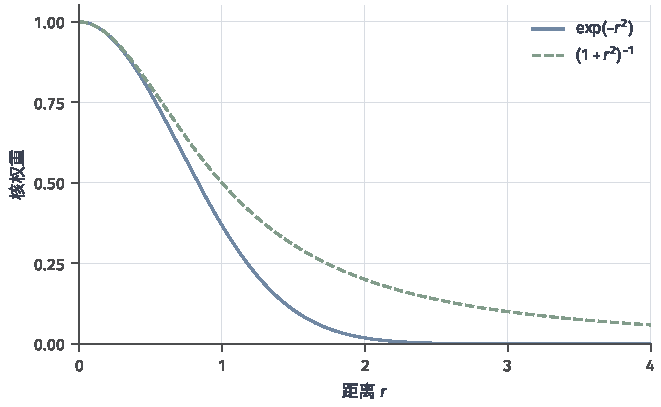
\includegraphics[width=105.412mm]{figures/04-classic-models/00-shared/matplotlib/dim-neighbor-tails/figure.pdf}
  \caption{高斯核$\exp(-r^2)$与Cauchy形核$1/(1+r^2)$的尾部。横轴$r$为无量纲距离，纵轴为未归一化核值，非概率密度、非实验结果；尾部形状本身不保证嵌入保真。}
  \label{fig:dim-neighbor-tails}
\end{figure}

\paragraph{收敛性}
坐标目标非凸，平移、旋转和反射也使坐标解不唯一。梯度光滑且步长合适时，可研究下降与趋近驻点；任意初始化的全局收敛仍无保证。即使谱方法全局解出固定图的子问题，图是否表达真实几何也要另行判断。

\paragraph{泛化性}
标准SNE没有共享输入映射，输出的是固定样本的坐标。其KL目标可以解释为该对象集上的邻居预测风险：先均匀抽取$I$，再按高维条件分布$p_{j\mid I}$抽取邻居$J$，用低维概率预测这一选择。交叉熵风险满足
\[
 R_G(\bm Z)=\mathbb E[-\log q_{J\mid I}]
 =\frac1n\sum_iH(p_{\cdot\mid i})+\frac1nC_{\mathrm{SNE}}(\bm Z).
\]
固定高维分布后，熵项不随坐标改变；若KL目标距全局最小值至多为$e_G$，就有
$R_G(\widehat{\bm Z})\leq\inf_{\bm Z}R_G(\bm Z)+e_G/n$。
该风险中的随机对象是已有样本索引，不能把训练样本间的$n(n-1)$个关系视作独立新观测。要处理新点，须另定参考邻域、旧坐标是否固定，以及新点损失；原始KL目标没有给出这种扩展的总体保证。输入关系主要来自噪声时，充分优化仍可能只是保留噪声关系。

\subsubsection{小结}

SNE先以困惑度校准邻域，再以条件概率和KL散度学习坐标。表示能力、布局优化和点对计算各有约束：更换核、改进优化与计算加速分别解决不同问题，需要分别评价。

\subsection{t-SNE}
\label{sec:dim-tsne}

SNE在低维空间用高斯距离构造邻居概率，高斯核随距离迅速衰减。高维中，一批点可以都离中心不远，彼此却分布在许多不同方向；把它们放到二维时，很难同时保留这些接近关系。若为了维持中等的相似度把许多点拉向中心，它们就会相互挤近，这就是拥挤问题的一种表现。

van der Maaten与Hinton于2008年提出\term{t-SNE}（t-distributed stochastic neighbor embedding），把低维核换为衰减较慢的重尾形式，并将逐点条件分布改为对称点对分布\scite{dim-vandermaaten2008tsne}重尾核允许中等相似度的点对在低维中相距更远，从而给重要近邻留下布局空间；对称化则让两个方向的邻居关系进入同一项损失。这些改变缓解了布局限制，却没有使二维坐标成为所有高维距离的等比例缩小。

\subsubsection{模型结构}

沿用高维条件概率与困惑度，为每对样本构造一个对称权重：
\begin{equation}
  \label{eq:dim-tsne-joint}
  \begin{aligned}
    p_{i,j}&=\frac{p_{j\mid i}+p_{i\mid j}}{2n},\qquad i\ne j,\\
    p_{i,i}&=0,\qquad p_{i,j}=p_{j,i},\qquad
      \sum_{i\ne j}p_{i,j}=1.
  \end{aligned}
\end{equation}
求和包括有序对的两个方向。$n$个条件分布各归一化为$1$，两方向相加后的总和为$2n$，因此分母取$2n$。若改按$i<j$求和，归一化及后续导数系数也需调整。

低维点对采用Cauchy形核，并在全部有序对上归一化：
\begin{equation}
  \label{eq:dim-tsne-low}
  \begin{aligned}
    u_{i,j}&=(1+r_{i,j}^2)^{-1},\qquad
      \mathcal{Z}=\sum_{a\ne b}u_{a,b},\\
    q_{i,j}&=\frac{u_{i,j}}{\mathcal{Z}},\qquad i\ne j,\\
    q_{i,i}&=0,\qquad \sum_{i\ne j}q_{i,j}=1.
  \end{aligned}
\end{equation}
$u_{i,j}$具有自由度为$1$的一维Student $t$核形状，$q_{i,j}$则是有限点对上的离散概率。重尾允许较远点获得相似度，未规定高低维距离相等，也未将$q_{i,j}$定义为$\mathbb{R}^k$上的多元Cauchy密度。

记$\bm{P}=(p_{i,j})$、$\bm{Q}=(q_{i,j})$，以点对分布间的KL散度学习坐标：
\begin{equation}
  \label{eq:dim-tsne-loss}
  C_{\mathrm{tSNE}}(\bm{Z})
    =\sum_{i\ne j}p_{i,j}\log\frac{p_{i,j}}{q_{i,j}}.
\end{equation}
全部点对共享归一化常数$\mathcal{Z}$。移动一个点会改变它和其他点的核值，也改变其余点对的概率，所以坐标要在共同概率预算下协调。

高概率近邻错置受到较大惩罚，簇间距离、面积和密度却未被要求复原。小$p_{i,j}$的吸引弱，但这些点对仍参与归一化与斥力计算，局部目标也需要考虑远点。

\subsubsection{参数学习}

代入低维核并利用$\sum_{i\ne j}p_{i,j}=1$，展开目标与归一化项的梯度：
\begin{equation}
  \label{eq:dim-tsne-gradient-derivation}
  \begin{aligned}
    C_{\mathrm{tSNE}}
      &=\text{常数}
        +\sum_{a\ne b}p_{a,b}\log(1+r_{a,b}^2)
        +\log\mathcal{Z},\\
    \nabla_{\bm{z}_i}\mathcal{Z}
      &=-4\sum_{j\ne i}u_{i,j}^2(\bm{z}_i-\bm{z}_j),\\
    \nabla_{\bm{z}_i}\log\mathcal{Z}
      &=-4\sum_{j\ne i}q_{i,j}u_{i,j}(\bm{z}_i-\bm{z}_j).
  \end{aligned}
\end{equation}
距离平方的导数贡献因子$2$，有序对的两个方向再贡献因子$2$。吸引项同理给出$4\sum_{j\ne i}p_{i,j}u_{i,j}(\bm{z}_i-\bm{z}_j)$，因此
\begin{equation}
  \label{eq:dim-tsne-gradient}
  \nabla_{\bm{z}_i}C_{\mathrm{tSNE}}
    =4\sum_{j\ne i}(p_{i,j}-q_{i,j})u_{i,j}
      (\bm{z}_i-\bm{z}_j).
\end{equation}
$p_{i,j}>q_{i,j}$时，负梯度拉近点对，反之推开。即使稀疏近似中$p_{i,j}=0$，有限距离的$q_{i,j}$仍为正，因而仍有斥力。每个点的位移由全部点对作用合成。

\term{早期夸大}（early exaggeration）在初始阶段将梯度中的$p_{i,j}$乘以$\alpha>1$，增强吸引后再恢复$\alpha=1$。原文使用$4$，后续也常用$12$，但需与学习率及样本数配合。夸大后权重和为$\alpha$，该阶段的更新已不是原归一化分布间KL散度的梯度。

初始化和动量也影响优化。缩放后的PCA坐标提供结构化起点，随机点云则不带这一信息；因此宏观布局差异可能同时来自起点与目标。动量未保证逃离局部极小值。实验应记录困惑度、学习率、初始化和夸大系数及轮数。

\subsubsection{理论分析}
\label{sec:dim-tsne-theory}

\paragraph{表达能力}
t-SNE扩大了中距离关系可以使用的布局范围，却仍通过同一组欧氏坐标耦合全部点对。若目标值为零，就必须有$q_{i,j}=p_{i,j}$；由式\eqref{eq:dim-tsne-low}可得
\[
 r_{i,j}^2=\frac{1}{\mathcal Z p_{i,j}}-1\qquad(i\ne j).
\]
因此只有存在一个共同的$\mathcal Z>0$，使这些平方距离经双中心化后得到的Gram矩阵半正定且秩至多为$k$，全部概率才能精确匹配。反过来，若这些距离可实现，核值为$\mathcal Zp_{i,j}$，全点对归一化就恰好恢复$\bm P$。重尾改变了概率对应的距离，却没有免除这一共同的几何约束。

高维高斯邻域经对称化后得到的目标概率，并不自动满足上述条件，二维或三维目标因而可能只能近似拟合。由于拟合对象是经过尺度调整的点对概率，视觉上分离的簇、簇面积和间距都可能来自布局目标，原空间未必具有相同密度或距离比例。

\paragraph{收敛性}

坐标目标仍非凸。Linderman与Steinerberger在2019年SIAM期刊论文中，针对有适当簇结构的输入相似度、集中初始点云及满足条件的步长和夸大系数，分析早期簇内收缩与谱聚类的联系\scite{dim-linderman2019clustering}结论针对该阶段和条件，未覆盖任意数据的整个训练。

初始间距小时，$u_{i,j}\approx1$。若斥力扰动相对较小并暂不计动量，更新近似为
\begin{equation}
  \label{eq:dim-tsne-spectral-approximation}
  \begin{aligned}
    \bm{Z}^{(t+1)}
      &\approx(\bm{I}-4\eta_t\alpha\bm{L}_{P})\bm{Z}^{(t)},\\
    \bm{L}_{P}&=\bm{D}_{P}-\bm{P},\qquad
    (\bm{D}_{P})_{i,i}=\sum_{j\ne i}p_{i,j}.
  \end{aligned}
\end{equation}
对角矩阵$\bm{D}_{P}$记录行和。步长合适时，图平滑抑制快速变化方向，因而与拉普拉斯谱相联系。点云展开后，核值接近$1$的近似会减弱，斥力也更不可忽略；关闭夸大后，布局仍由两种作用共同调整。

\paragraph{泛化性}
固定高维联合点对分布$p_{ij}$，抽取$(I,J)\sim p$后用$q_{ij}(\bm Z)$预测，交叉熵风险为
\[
 R_G(\bm Z)=\mathbb E_{(I,J)\sim p}[-\log q_{IJ}(\bm Z)]
           =H(p)+C_{\mathrm{tSNE}}(\bm Z).
\]
所以完整KL目标距全局最小值至多为$e_G$时，有
$R_G(\widehat{\bm Z})\leq\inf_{\bm Z}R_G(\bm Z)+e_G$。
这是固定对象集的点对风险，较小训练KL只回答该邻居预测任务；点对分布由同一批数据产生，不能据此断言独立新点上的期望风险小。参数化t-SNE虽然给出了输入映射，还需规定总体点对采样与归一化制度，并控制函数族的复杂度；前向计算本身没有提供风险界。


困惑度决定输入分布，也决定所求问题。小值强调细邻域，可能割裂连续结构；大值引入更广关系，可能模糊稀有群体。可在可达范围内比较$5$、$30$、$50$等尺度及多次初始化，寻找稳定关系。不同困惑度对应不同目标分布，其KL值不能直接用于排名。

旋转和镜像通常不改变解释，簇间距、面积及疏密却也不能直接换算为原空间量。布局可能展开大簇、压紧小簇，或将连续变化分成区域。单细胞、文本或图像特征中的分组应回到合适的高维表示验证，并分别考察内部指标、稳定性、参考标签及下游效果（参见第\ref{sec:clustering-summary}节）。

\subsubsection{优化计算能力}

原始算法每轮需$O(n^2)$计算。van der Maaten在2014年的Barnes--Hut t-SNE中将吸引图稀疏化，并用低维树聚合远点、近似斥力，二维常用四叉树。固定近邻预算及近似精度、输出维数较小时，每轮典型成本为$O(n\log n)$；建图及极端布局仍会影响时间\scite{dim-vandermaaten2014accelerating}

Linderman等在2019年的FIt-SNE中通过网格插值和快速傅里叶变换加速核求和\scite{dim-linderman2019fitsne}。固定插值阶数时，斥力成本约为$O(n+g\log g)$，其中$g$为网格节点数，此外还需计算稀疏吸引。范围与精度改变时$g$也会改变。2019年工作展示了百万级单细胞数据的处理，实际规模与收益仍依赖计算条件。

\subsubsection{支持新样本低维编码场景}

新点需要额外扩展规则。openTSNE等实现固定参考坐标，再按新点与参考样本的相似度优化新坐标\scite{dim-policar2024opentsne}。这是条件定位，与新旧样本联合训练不同；参考集未覆盖的新群体可能被安排到失真位置。

需要反复处理新样本时，可令$\bm{z}_i=f_{\bm{\theta}}(\bm{x}_i)$，按邻域目标学习共享参数。van der Maaten于2009年提出参数化t-SNE，以前向计算表示新点\scite{dim-vandermaaten2009parametric}。网络函数族限制可实现布局，批次构造与归一化也影响训练关系。

\subsubsection{小结}

t-SNE用对称点对分布和重尾核组织局部相似性，适合探索邻域。它重视保留高概率关系，簇间距离、面积和疏密却不宜直接换算成原空间量；困惑度与初始化也会改变所显示的结构。

计算加速与新点编码处理不同瓶颈。Barnes--Hut用树近似远点作用，FIt-SNE用网格插值加速核求和，两者都需选择近似精度。固定参考表示后优化新点，可以复用既有坐标；参数化t-SNE改为学习共享输入函数，减少逐点定位，同时让函数族与训练方式限制可实现布局。这些调整方便计算和使用，结构解释仍需回到原表示验证。

\subsection{UMAP}
\label{sec:dim-umap}

SNE和t-SNE把邻域相似度组成归一化概率分布，目标是匹配这些分布。另一种表示方式是直接为每条局部连接赋予强度：两个样本在各自邻域里有多接近，就决定这条连接有多强，全部点对的权重不需要加起来等于1。\term{统一流形逼近与投影}（uniform manifold approximation and projection，UMAP）先按各点的局部距离尺度建立加权邻域，再合并两端对同一连接的判断，得到一张稀疏图。低维布局随后拟合这些连接强度，让强连接的点靠近，并对其他点对施加排斥。它延续了邻域表示的目标，但改变了高维关系的构造与拟合方式。

McInnes、Healy与Melville自2018年公开的方法长文，将拉普拉斯特征映射、黎曼几何与模糊拓扑联系起来，讨论非均匀样本的局部度量及其合并\scite{dim-mcinnes2018umap}这一构造也面向较高维预处理。方法长文与同年JOSS软件论文分别描述理论构造和实现，几何解释、实现行为与可视化效果应各自评价。

\subsubsection{模型结构}

以$N_q(i)$表示不含$i$的$q$个近邻。先取互异样本、无并列最近邻及单位局部连接设置。记$\rho_i=\min_{j\ne i}\delta_{i,j}$，定义有向权重
\begin{equation}
  \label{eq:dim-umap-directed}
  \begin{aligned}
    v_{j\mid i}
      &=
      \begin{cases}
        \exp\!\left(-\dfrac{\max(0,\delta_{i,j}-\rho_i)}
        {\sigma_i}\right),&j\in N_q(i),\\
        0,&j\notin N_q(i),
      \end{cases}\\
    \sum_{j\in N_q(i)}v_{j\mid i}&=\log_2 q.
  \end{aligned}
\end{equation}
偏移$\rho_i$使最近邻权重为$1$，带宽$\sigma_i$控制其余边衰减。上述条件下，$q>2$时权重和随带宽从$1$趋向$q$，可搜索满足目标的带宽。距离可按任务更换，相应的几何解释也需要调整。

这些值是边的隶属强度，多条边可同时很强。校准目标$\log_2 q$未将行和设为$1$，也未使用熵或困惑度。重复或并列样本、其他局部连接设置可能使多条边固定为$1$，导致目标不可达，因而实现还需处理零距离、带宽下界与容差。

用模糊并将两个方向合成对称权重：
\begin{equation}
  \label{eq:dim-umap-union}
  v_{i,j}=v_{j\mid i}+v_{i\mid j}-v_{j\mid i}v_{i\mid j}.
\end{equation}
所得$v_{i,j}=v_{j,i}\in[0,1]$。一方向为$1$则合并为$1$，两方向均为$0.4$则合并为$0.64$。这是模糊集合运算，无需把两条边假定为独立事件。

\term{模糊单纯集}（fuzzy simplicial set）将点、边和三角面等组合结构赋予隶属强度，提供局部描述的组合框架。实际目标主要使用样本与加权边，即一维骨架。有限图中的环和空白是否对应真实拓扑，仍需采样与几何证据。

低维边强度由可调重尾核给出：
\begin{equation}
  \label{eq:dim-umap-kernel}
  w_{i,j}=\frac{1}{1+a r_{i,j}^{2b}},\qquad a>0,\quad b>0.
\end{equation}
由\code{min\_dist}和\code{spread}选择$a,b$，使光滑核逼近近处接近$1$、超过指定尺度后衰减的曲线。\code{min\_dist}允许控制紧凑程度，未给每对点施加硬距离下界。$a=b=1$时核形与t-SNE的$u_{i,j}$相同，但没有全局归一化，因而与$q_{i,j}$不同。

将每条边视为带软标签的二元判断，就可以匹配高低维边强度。按无序对$i<j$写完整目标：
\begin{equation}
  \label{eq:dim-umap-bernoulli}
  \begin{aligned}
    C_{\mathrm{B}}(\bm{Z})
      &=\sum_{i<j}\left[
        v_{i,j}\log\frac{v_{i,j}}{w_{i,j}}\right.\\
      &\qquad\left.+
        (1-v_{i,j})\log\frac{1-v_{i,j}}{1-w_{i,j}}
        \right].
  \end{aligned}
\end{equation}
该式求和逐边Bernoulli分布的KL散度。去掉只依赖高维权重的常数，得到二元交叉熵：
\begin{equation}
  \label{eq:dim-umap-cross-entropy}
  \begin{aligned}
    C_{\mathrm{CE}}(\bm{Z})
      &=-\sum_{i<j}\left[
        v_{i,j}\log w_{i,j}\right.\\
      &\qquad\left.+
        (1-v_{i,j})\log(1-w_{i,j})\right].
  \end{aligned}
\end{equation}
采用$0\log0=0$。两式对坐标有相同梯度，所以与t-SNE的核心区别在匹配对象：这里逐边二元匹配，t-SNE匹配全局归一化的点对分布。

正边项吸引，非边项排斥。$v_{i,j}=0$只说明局部图未保留这条连接，未区分稍远与极远的点对，因此该目标未规定全局距离保真。

\subsubsection{参数学习}

连接强度取决于点对距离，因此学习坐标时可以沿损失的负梯度移动点。为了看清一次更新怎样拉近或推开一对样本，分别记吸引损失$\ell^+_{i,j}=-\log w_{i,j}$与排斥损失$\ell^-_{i,j}=-\log(1-w_{i,j})$。把前面给出的$w_{i,j}$代入，对$\bm z_i$求导；当点对距离$r_{i,j}>0$时，得到
\begin{equation}
  \label{eq:dim-umap-pair-gradient}
  \begin{aligned}
    \nabla_{\bm{z}_i}\ell^+_{i,j}
      &=\frac{2ab r_{i,j}^{2b-2}}
        {1+a r_{i,j}^{2b}}(\bm{z}_i-\bm{z}_j),\\
    \nabla_{\bm{z}_i}\ell^-_{i,j}
      &=-\frac{2b}
        {r_{i,j}^2(1+a r_{i,j}^{2b})}
        (\bm{z}_i-\bm{z}_j).
  \end{aligned}
\end{equation}
两项负梯度分别拉近与推开点对，完整目标再按$v_{i,j}$与$1-v_{i,j}$加权。接近重合时排斥项奇异，计算需稳定处理并控制更新幅度。

全点对计算仍为二次规模。\term{负采样}（negative sampling）按正边权重安排吸引，再为中心点抽$s$个排斥对象，抽样未逐个检查它们是否为非邻居。若图有$O(nq)$条边，每边每轮更新次数有界、$k$固定，一轮约需$O(nq(1+s))$；近似线性还要求$q,s$固定，并未包含建图和总轮数。

中心的更新频率取决于正边权重，负样本频率取决于采样分布。缺少重要性修正时，期望更新一般不同于完整交叉熵梯度，吸引与排斥的相对强度也随之改变。

Damrich与Hamprecht于2021年分析有效更新。令$\omega_i=\sum_{j\ne i}v_{i,j}$。在均匀负采样且排斥更新双端的模型下，略去共同正常数，有效目标为
\begin{equation}
  \label{eq:dim-umap-effective-loss}
  \begin{aligned}
    \widetilde C(\bm{Z})
      &=\sum_{i<j}\left[
        v_{i,j}\ell^+_{i,j}
        +\gamma_{i,j}\ell^-_{i,j}\right],\\
    \gamma_{i,j}&=\frac{s(\omega_i+\omega_j)}{2n}.
  \end{aligned}
\end{equation}
排斥系数由样本数、加权度和采样数决定，已不同于$1-v_{i,j}$。原文分析的非参数实现只移动排斥对的一端，其期望更新一般甚至没有对应的标量损失；上式仅适用于补上双端更新的版本\scite{dim-damrich2021umaploss}

暂将各$w_{i,j}$视为独立变量，其最优值为$v_{i,j}/(v_{i,j}+\gamma_{i,j})$。正边权重远大于排斥系数时，该值接近$1$，解释了部分紧凑布局倾向。实际坐标耦合全部边强度，未必能同时达到这些逐边最优值。负采样改变了吸引与排斥的比例，因此其逐边偏好也不同于完整目标中的$v_{i,j}$。

实现先搜近邻、估计尺度、合并图，再初始化并作采样更新。可取谱或随机初始化；断连分量之间缺少相对位置约束。学习率衰减、负样本数和排斥强度也影响布局，需与主要参数一起记录。

\code{n\_neighbors}控制连接尺度，较大值加入更广关系。\code{min\_dist}小允许紧凑群组，大则通常更分散，但这些变化未保证评价指标单调改善。\code{umap-learn}常用$q=15$、\code{min\_dist=0.1}作为起点；还需记录度量、维数、轮数、种子及版本\scite{dim-mcinnes2018umapsoftware}

\subsubsection{理论分析}
\label{sec:dim-umap-theory}

\paragraph{表达能力}
UMAP的低维候选边强度由一组$k$维坐标共同决定，不能逐边独立设置。对$0<v_{i,j}<1$的边，完整Bernoulli匹配误差为零要求$w_{i,j}=v_{i,j}$，对应距离为
\[
 r_{i,j}=\left(\frac{v_{i,j}^{-1}-1}{a}\right)^{1/(2b)}.
\]
这些距离还须共同满足欧氏几何及维数限制。权重为$1$的边要求端点重合；例如一条三点链的两条边权重均为$1$，两次重合会迫使首尾也重合，便不能同时表达首尾权重为$0$。权重为$0$又要求无限远才能使重尾核严格为零，所以常见稀疏图在有限坐标中一般只能近似匹配完整目标。

局部图只提供连接尺度，未规定全局距离、密度或可逆性。图中没有保留的远距离信息，也不能由布局补回。

\paragraph{收敛性}

完整交叉熵及有效采样目标都对坐标非凸，近邻近似、有限轮更新和梯度裁剪还会改变求解行为。趋近驻点的条件结论仅涉及给定目标，未保证最佳拓扑布局。负采样分析解释有效吸引与排斥，也未建立与非负矩阵分解的等价或相对t-SNE的普遍优势。

\paragraph{泛化性}
完整交叉熵对应一个明确的有限图任务。令$N=n(n-1)/2$，均匀抽取无序节点对$(I,J)$，再抽取$A_{IJ}\sim\operatorname{Bernoulli}(v_{IJ})$，以$w_{IJ}(\bm Z)$预测边是否存在。其期望对数损失为
\[
 R_G(\bm Z)=\mathbb E[-A_{IJ}\log w_{IJ}
                  -(1-A_{IJ})\log(1-w_{IJ})]
           =C_{\mathrm{CE}}(\bm Z)/N.
\]
若完整交叉熵的求解误差为$e_G$，则
$R_G(\widehat{\bm Z})\leq\inf_{\bm Z}R_G(\bm Z)+e_G/N$。
采样分布在此由冻结的图规定，并非未知总体中的独立新对象。常用负采样的期望更新与完整交叉熵不同，也没有给出其全局求解误差，因而不能将这一结论直接归给默认实现。


局部流形、尺度调整和模糊拼接说明图如何构造。有限样本结果仍依赖光滑几何、合适度量与足够采样；理论构造、近似建图和采样求解各有条件，不能直接将一层的保证用于另一层。

\subsubsection{优化计算能力}

样本很多时，可以先用子样本拟合参考布局，再定位其余点，减少联合优化的位置数。子样本需要覆盖稀有群体等重要关系；若参考表示已经遗漏这些关系，后续定位就缺少相应依据。节省拟合计算的同时，还需计入剩余样本的近邻查询与定位成本。

\subsubsection{支持新样本低维编码场景}

\code{transform}先在训练集找新点邻居，以邻居坐标初始化，再固定参考表示优化新点。这是给定参考图的条件定位。新数据接近训练分布时可借此放入同一图；新类别或分布漂移却可能使位置失真。

共享输入函数提供另一种扩展。Sainburg、McInnes与Gentner的参数化UMAP以正负样本训练网络，支持小批次和半监督学习\scite{dim-sainburg2021parametricumap}。它通过前向计算处理新点，与固定参考图后优化位置不同；分布外泛化及对非参数布局的复现仍需验证。

\subsubsection{小结}

UMAP按局部尺度构造加权邻域图，再以可调核安排坐标。边强度、完整匹配目标与采样更新承担不同作用；度量、近邻近似、初始化及采样都会影响参考表示，需要按所用实现记录并解释。

接收新样本时，固定参考图后的条件定位与参数化UMAP是两条路线。前者复用参考邻域，却仍需求新点位置，并依赖参考集覆盖；后者用共享网络前向编码，减少逐条优化，也增加函数族、训练和布局复现的限制。用于下游预测时，应将这些表示学习步骤放入训练划分，并直接评价任务效果。

\subsection{最大方差展开（MVU）}

卷起的纸展开时，纸面上的内在距离保持不变；在足够小的区域内，空间中的直线距离可以近似这一长度。将局部边长保持作为约束，有助于展开时让隔着不同卷层的点分开。\term{最大方差展开}（maximum variance unfolding, MVU）把这一关系直接写成约束：固定近邻边的长度，同时尽量增大整批坐标的总方差。

\subsubsection{模型结构}

MVU不先用最短路径估计远距离，而是优化未知Gram矩阵$\bm{B}$：
\[
  \begin{aligned}
    \max_{\bm{B}\succeq0}\quad&
      \operatorname{tr}(\bm{B}),\qquad \bm{B}\bm{1}=\bm{0},\\
    \text{满足}\quad&
      \bm{B}_{i,i}+\bm{B}_{j,j}-2\bm{B}_{i,j}
      =\lVert\bm{x}_i-\bm{x}_j\rVert_2^2,\quad(i,j)\in E.
  \end{aligned}
\]
中心化时，增大迹就是在保持局部边长下增大总方差。

\subsubsection{参数学习}
先求解上述凸半正定规划，再对最优Gram矩阵作特征分解，以特征向量乘相应特征值平方根构造坐标。若只输出$k$维，就保留前$k$个方向；这一步截断与半正定规划是两个不同步骤\scite{dimWeinberger2006}。

\subsubsection{理论分析}

\paragraph{表达能力}
任意中心化欧氏坐标都对应一个半正定Gram矩阵。若目标坐标保持全部指定边长，它就在未限制秩的可行集中；要在$k$维中精确表示，还要求存在秩至多为$k$的可行矩阵。原始坐标本身总能提供一个可行解，却不保证低维可行解存在。最优矩阵若秩大于$k$，截断通常缩短一些边，原先精确满足的局部距离约束便可能失效。即使边长全部保持，稀疏图也可能允许多种折叠，目标几何未必唯一。

\paragraph{收敛性}
若邻域图连通，任意两点的距离受连接路径的边长之和控制，所有坐标又要求中心化，故可行Gram矩阵有界。可行集非空且闭，线性迹目标就能取得最大值。图若断连，则可沿相反方向平移不同分量并保持整体中心化，边长约束不变而迹无限增大，原问题可能无有限最优值。连通情形可用凸半正定求解器计算原始、对偶可行解及间隙；给定可行性与间隙容差才有可核查的求解精度。若额外加入秩不超过$k$的约束，就不再是原来的凸问题，不能继续沿用凸求解保证。

\paragraph{泛化性}
MVU只为当前对象优化坐标，没有直接给出新点映射。因而训练边长全部保持，仍不足以估计未见点对的几何误差。若部署时另外冻结一个编码器$f$，可以对独立的新点对$(\bm X,\bm X')$评价距离失真。假设输入范数至多为$r$、输出范数至多为$a$，采用
\[
 \ell_f(\bm X,\bm X')=
 \left(\lVert f(\bm X)-f(\bm X')\rVert_2^2
            -\lVert\bm X-\bm X'\rVert_2^2\right)^2,
 \qquad R(f)=\mathbb E\ell_f.
\]
损失不超过$B=16\max\{r^4,a^4\}$。对独立于拟合过程的$m$个独立同分布点对，以至少$1-\delta$的概率有
\[
 R(f)\leq\widehat R_m^{\mathrm{val}}(f)
        +B\sqrt{\frac{\log(1/\delta)}{2m}}.
\]
这是冻结编码器的期望几何误差估计，并非MVU训练约束推出的保证。同一批点构成的全部点对相互依赖，不能将其数量直接代入这里的$m$；若目标是内在测地距离，也需把损失中的欧氏距离换成相应目标并重新核对有界条件。

\subsection{模型对比与总结}
\label{sec:dim-manifold-comparison}
\label{sec:dim-neighbors-comparison}

基于邻域的方法首先要决定局部关系怎样约束整体。Isomap把可信邻域串成路径，再用MDS安排全局坐标；它回应欧氏直线会穿过弯曲结构、不能表示沿曲面距离的问题。代价是许多远点距离都依赖图路径，一条错误连接就可能改变大量点对关系。LLE不估计全局路径，改为保留每个样本由邻居重构的仿射关系，局部矩阵是否稳定及邻域是否充分重叠因而成为关键。

局部重构还可以按展开要求细化。Hessian LLE约束坐标函数的二阶变化，LTSA估计各块切空间，再用重叠样本协调局部坐标。前者需要更充分的局部采样来估计曲率，后者把误差集中到切方向估计和坐标拼接；两者都没有通过增加算法步骤消除邻域本身缺少的信息。

拉普拉斯特征映射与扩散映射从另一种局部关系进入：边权只表明哪些点应相近。前者使坐标沿强连接平缓变化，后者把连接组织成随机传播，再比较给定时间内到达各处的概率。扩散时间提供了局部与较大尺度之间的调节，密度归一化则决定传播主要保留采样密度还是几何；两项选择也可能削弱任务希望保留的差异。表\ref{tab:dim-manifold-comparison}汇总这些保留对象和新点机制，MDS与核PCA在其中作为全局关系的参照。

\begin{table*}[htbp]
  \centering
  \small
  \begin{tabularx}{\linewidth}{@{}>{\RaggedRight\arraybackslash}p{22mm}>{\RaggedRight\arraybackslash}X>{\RaggedRight\arraybackslash}X>{\RaggedRight\arraybackslash}X@{}}
    \toprule
    方法 & 输入与保留对象 & 核心求解 & 样本外使用与主要限制 \\
    \midrule
    MDS & 给定差异；经典型拟合内积，应力型拟合距离或顺序
      & 经典型取正谱；度量及非度量应力通常迭代求解
      & 需要到训练点的差异；非欧氏性与目标维数限制保真程度 \\
    核PCA & 正定核；特征空间方差
      & 中心化核矩阵的主特征方向
      & 核投影有明确公式；依赖训练中心化、核尺度和谱隙 \\
    Isomap & 邻域图；全局测地距离的估计
      & 最短路径后做经典MDS
      & 接入图后做距离扩展；短路、断连及不可展开几何会失真 \\
    LLE & 邻居与局部重构权；仿射重构关系
      & 局部线性方程与全局低端谱
      & 局部权重插值；病态邻域、多零模态与噪声需诊断 \\
    Laplacian Eigenmaps & 对称非负邻域权重；图上平滑性
      & 度加权广义特征值问题
      & 可作谱延拓；度、密度、断连影响低频表示 \\
    Diffusion Map & 对称权重及重加权；给定步数的扩散距离
      & 满足细致平衡的转移矩阵谱与时间加权
      & Nystr\"om延拓；截断、带宽和过度混合限制区分能力 \\
    \bottomrule
  \end{tabularx}
  \caption{六类方法在本节所述标准构造下的比较。MDS一行区分经典型与应力型，不能把二者的目标和求解混同。样本外一栏均指固定训练表示后的扩展，不代表加入新样本重新训练的等价结果，也不是预测性能保证。}
  \label{tab:dim-manifold-comparison}
\end{table*}

如果目标主要是展示邻居关系，可以直接匹配高维与低维的相似性，而不要求恢复流形距离。SNE采用逐点条件邻居分布，低维高斯核却难以给中等相似的邻居同时留下足够空间。t-SNE改用对称点对分布与重尾低维核，让这类关系在更远位置仍有相似性，缓解拥挤；它仍没有要求簇间距离、面积或密度复原。

UMAP也使用吸引与排斥安排邻域，但先用逐点尺度构造稀疏模糊图，低维边权不作t-SNE式的全局概率归一化。其交叉熵与常用负采样还需分别解释。因此，UMAP与t-SNE是对邻域关系的不同建模和求解，不能仅凭图形相似就认定它们优化同一个目标。表\ref{tab:dim-neighbors-comparison}列出这些差别；困惑度与建图邻居数$q$都影响尺度，但并非可以直接互换的参数。

大规模布局还可以改变计算或关系的覆盖。Barnes--Hut与FIt-SNE近似t-SNE的远点作用，LargeVis联合近似建图与概率布局\scite{dim-tang2016largevis}。它们减少的计算步骤及近似目标各不相同。

只靠近邻难以确定不同局部区域的相对位置，PaCMAP让中距离关系也参与分阶段定位\scite{dim-wang2021pacmap}。TriMap改用跨尺度三元组比较相对远近，为区域之间增加距离顺序约束\scite{dim-amid2019trimap}。增加跨尺度约束改变了重点保留的关系，也增加配对或三元组选择的影响，仍需检查实际输入中这些关系是否可信。

\begin{table*}[tbp]
  \centering
  \small
  \begin{tabularx}{\linewidth}{@{}p{0.13\linewidth}>{\RaggedRight\arraybackslash}X>{\RaggedRight\arraybackslash}X>{\RaggedRight\arraybackslash}X@{}}
    \toprule
    比较方面 & SNE & t-SNE & UMAP \\
    \midrule
    高维对象 & 逐点条件邻居概率 & 对称联合点对概率 & 稀疏模糊邻域图权重 \\
    低维对象 & 行归一化高斯核 & 全局归一化重尾核 & 不作概率归一化的可调重尾权重 \\
    建模依据 & 条件分布匹配 & 点对分布匹配 & 局部几何与模糊图构造 \\
    优化目标 & 条件KL散度之和 & 联合KL散度 & 逐边交叉熵；负采样改变有效目标 \\
    邻域尺度 & 困惑度及逐点带宽 & 困惑度及逐点带宽 & 邻居数$q$、局部距离偏移和带宽 \\
    布局控制 & 初始化、学习率等 & 初始化、夸大、学习率等 & 初始化、核形状、采样和排斥等 \\
    迭代代价 & 稠密计算$O(n^2)$ & 稠密$O(n^2)$；树或插值可加速 & 固定嵌入维数下约$O(nq(1+s))$ \\
    全局解释 & 不保证距离或密度保真 & 簇间距、面积不宜直接解释 & 图连接提供约束，但不保证全局保真 \\
    新样本 & 需另定义扩展 & 参考图扩展或参数化版本 & \code{transform}或参数化版本 \\
    \bottomrule
  \end{tabularx}
  \caption{三种邻域降维方法。复杂度指固定嵌入维数下的一轮优化，不含建图和总轮数；$s$为每次正边更新的负采样数。}
  \label{tab:dim-neighbors-comparison}
\end{table*}

比较速度时应固定近邻搜索、近似精度、硬件、线程及优化预算，才能解释差异。预处理、初始化、版本与并行方式也影响复现。固定种子便于重跑，多种子和多尺度则用于检查结构稳定性。

探索图形可以用于提出假设或展示已有分析支持的结构，簇数、大小与间隔仍需在原始或合适的高维表示中检验。用于下游特征时，嵌入不必固定为二维，应按任务选择维数，并检查不同尺度与初始化下的结果。

\section{基于概率的降维}
\label{sec:dim-probabilistic}

概率降维先规定低维因素如何生成观测，再用观测推断这些因素。PPCA、FA与GPLVM分别改变映射、噪声或未知量的处理方式，均沿用$n,d,k$及输入矩阵$\bm{X}$。这一生成视角与第\ref{sec:classic-overview-probabilistic}节的潜变量建模相联系。

\subsection{概率主成分分析（PPCA）与因子分析}
\label{sec:dim-ppca}

回到多个传感器测量共同状态的例子。PCA选出了重构误差较小的子空间，却没有单独说明共同信号与读数噪声怎样生成。如果希望推断一个带噪读数背后的状态，或根据已有传感器读数估计缺失读数，就需要给出观测的概率模型。\term{概率主成分分析}（probabilistic principal component analysis, PPCA）以低维高斯状态生成线性信号，再叠加同方差高斯噪声。给定观测后，模型可以反过来计算潜在状态的后验，而不仅给出一次正交投影。

PPCA要求各观测坐标的噪声方差相同；如果一个传感器精度较高，另一个读数波动较大，这一设定就难以分别描述它们的误差。高斯\term{因子分析}（factor analysis, FA）把噪声协方差放宽为对角矩阵，允许各坐标有不同噪声方差，而共同变化仍由少数潜变量解释。“因子”就是这些解释共同变化的潜变量。历史可追溯到Spearman于1904年的一般智力研究，现代多因子模型的含义和范围已不同于当时的心理测量假说\scite{spearman1904intelligence}

Tipping与Bishop在1999年为PCA引入与因子分析相关的概率模型，以似然刻画主子空间并研究EM估计\scite{tipping1999}在同一似然下，谱解与潜变量迭代可以比较，噪声及缺失观测也可以纳入统计推断。

\subsubsection{模型结构}
\label{sec:dim-ppca-structure}

令$\bm{z}\in\mathbb{R}^k$为潜变量，$\bm{W}\in\mathbb{R}^{d\times k}$为载荷，$\bm{\mu}\in\mathbb{R}^d$为均值。PPCA取$1\leq k<d$，以独立的潜变量和噪声生成观测：
\begin{equation}
\label{eq:dim-ppca-generative}
\begin{aligned}
\bm{z}&\sim\mathcal{N}(\bm{0},\bm{I}_k),\\
\bm{x}&=\bm{\mu}+\bm{W}\bm{z}+\bm{\epsilon},\\
\bm{\epsilon}&\sim\mathcal{N}(\bm{0},\sigma^2\bm{I}_d),
\qquad \bm{\epsilon}\perp\bm{z},\quad \sigma^2>0.
\end{aligned}
\end{equation}
各向同性约束噪声方向，观测的总方差仍可不同。给定潜变量时，条件负对数似然含平方残差$\lVert\bm{x}-\bm{\mu}-\bm{W}\bm{z}\rVert_2^2/(2\sigma^2)$；拟合边缘似然则还要将潜变量积分掉。

图~\ref{fig:dim-latent-model}区分两个方向：生成时抽取潜变量并加噪声，编码时给定观测求潜变量后验。
\begin{figure}[htbp]
  \centering
  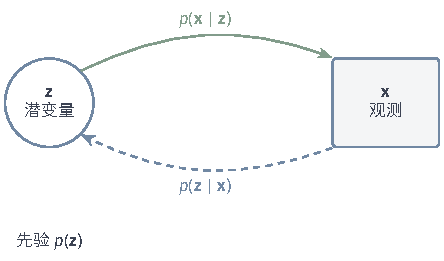
\includegraphics[width=75.188mm]{figures/04-classic-models/00-shared/tikz/dim-latent-model/figure.pdf}
  \caption{概率生成与后验推断的结构示意。实线表示$\bm{z}\to\bm{x}$的生成方向；虚线表示$\bm{x}\to\bm{z}$的后验推断，不是额外的生成依赖。图中节点与箭头只说明变量角色和条件关系，不表示实测数据、网络层数或计算流程；噪声描述观测对信号的偏离，不是新增的潜变量维数。}
\label{fig:dim-latent-model}
\end{figure}

独立高斯量线性组合仍为高斯量，将潜变量积分后得到
\begin{equation}
\label{eq:dim-ppca-marginal}
\begin{aligned}
p(\bm{x})&=\mathcal{N}(\bm{x};\bm{\mu},\bm{C}),\\
\bm{C}&=\bm{W}\bm{W}^\top+\sigma^2\bm{I}_d.
\end{aligned}
\end{equation}
信号协方差的秩至多为$k$，正噪声使$\bm{C}$正定；样本不足导致经验协方差奇异时，模型协方差仍可正定。

FA将噪声改为$\bm{\Psi}=\operatorname{diag}(\psi_1,\ldots,\psi_d)$，其中$\psi_j>0$为方差，故$\bm{C}=\bm{W}\bm{W}^\top+\bm{\Psi}$。给定因子，各维条件独立，跨维协方差由共同因子产生。独特方差也可包含特征自身的变化，解释时需结合测量机制；标准化会同时改变同方差假设的含义。

图\ref{fig:dim-ppca-fa-noise}固定载荷，只比较条件噪声。给定一个潜变量值，PPCA允许观测沿各方向等幅偏离均值，FA允许沿某坐标偏离更多。圆与椭圆均表示条件噪声；再混合不同潜变量值，才会加入信号协方差并形成总体分布。

\begin{figure}[htbp]
  \centering
  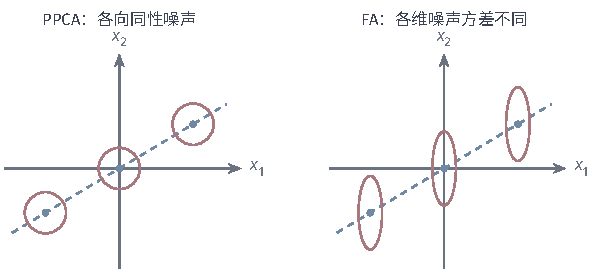
\includegraphics[width=101.840mm]{figures/04-classic-models/00-shared/tikz/dim-ppca-fa-noise/figure.pdf}
  \caption{PPCA与FA的条件噪声示意。设$d=2$、$k=1$、$\bm{\mu}=\bm{0}$、$\bm{W}=(1,0.6)^\top$，三个实心点对应$z=-1,0,1$的条件均值。左图取$\sigma=0.28$，右图取$\bm{\Psi}=\operatorname{diag}(0.16^2,0.50^2)$；每条轮廓到其中心的平方Mahalanobis距离均为$1$。坐标为无量纲构造值，轮廓是条件等密度线，不是总体数据云或置信区域。}
  \label{fig:dim-ppca-fa-noise}
\end{figure}

载荷的正交旋转$\bm{W}\bm{R}$不改变协方差。载荷满列秩且除旋转外局部可识别时，可扣除$k(k-1)/2$个旋转自由度：PPCA与FA的协方差参数数目分别为$dk+1-k(k-1)/2$及$dk+d-k(k-1)/2$，均值另有$d$个。FA还需排除载荷与噪声间的额外歧义。相较自由协方差的$d(d+1)/2$个参数，低秩约束可以降低估计方差，也可能带来模型偏差。

\subsubsection{参数学习}
\label{sec:dim-ppca-learning}

设样本独立同分布，均值为$\bar{\bm{x}}$，中心化量为$\bm{y}_i=\bm{x}_i-\bar{\bm{x}}$，记$\bm{S}=n^{-1}\sum_i\bm{y}_i\bm{y}_i^\top$。固定$\bm{C}$时，均值梯度$n\bm{C}^{-1}(\bar{\bm{x}}-\bm{\mu})$与负定二阶导数给出$\hat{\bm{\mu}}=\bar{\bm{x}}$。代回最大似然目标得
\begin{equation}
\label{eq:dim-ppca-likelihood}
\ell=-\frac{n}{2}\left[
d\log(2\pi)+\log|\bm{C}|
+\operatorname{tr}(\bm{C}^{-1}\bm{S})\right].
\end{equation}
对数行列式惩罚过大的协方差体积，迹项则惩罚在数据有较大变化的方向上赋予过小方差。

对$\bm{S}$作谱分解$\bm{U}\bm{\Lambda}\bm{U}^\top$，按$\lambda_1\geq\cdots\geq\lambda_d\geq0$排列。令$\bm{U}_k$包含前$k$个方向，$\bm{\Lambda}_k=\operatorname{diag}(\lambda_1,\ldots,\lambda_k)$。

证明需要比较两组谱的配对。Birkhoff--von Neumann分解说明：行和、列和均为$1$的非负方阵，即双随机矩阵，可以写成置换矩阵的凸组合\scite{birkhoff1946}因此双随机矩阵上的线性目标至少为某个置换取值的最小值。

最大似然解以PCA主方向构造载荷，以舍弃特征值的均值估计噪声，载荷内部保留旋转自由。下面先证明样本谱与模型谱同序配对最优，再优化谱值，从而说明全局最优性；奇异点及高维统计保证仍需另外讨论。

\begin{theorem}[PPCA最大似然解的存在条件与闭式表示]
\label{thm:dim-ppca-mle}
设$1\leq k<d$，尾谱均值$\tau=(d-k)^{-1}\sum_{j=k+1}^d\lambda_j$满足$\tau>0$且$\lambda_k>\tau$。在$\sigma^2>0$的PPCA模型中，以下参数达到全局最大似然：
\begin{equation}
\label{eq:dim-ppca-mle}
\begin{aligned}
\hat{\bm{\mu}}&=\bar{\bm{x}},\qquad
\hat{\sigma}^2=\tau,\\
\hat{\bm{W}}&=\bm{U}_k(\bm{\Lambda}_k-\tau\bm{I}_k)^{1/2}\bm{R}.
\end{aligned}
\end{equation}
其中$\bm{R}$为任意$k$阶正交矩阵。截断处有重根时，$\bm{U}_k$可在对应特征子空间内选取不同正交方向。
\end{theorem}

\begin{proof}
需最小化$F(\bm{C})=\log|\bm{C}|+\operatorname{tr}(\bm{C}^{-1}\bm{S})$。写$s=\sigma^2$，由信号半正定且秩至多为$k$，可行协方差的谱满足
\[
c_1\geq\cdots\geq c_k\geq s,\qquad
c_{k+1}=\cdots=c_d=s>0.
\]
允许$c_j=s$便包括载荷秩不足$k$的情况。

固定谱，设$\bm{p}_b$为$\bm{C}$的第$b$个单位特征向量，则
\[
\operatorname{tr}(\bm{C}^{-1}\bm{S})
=\sum_{a=1}^d\sum_{b=1}^d
\frac{\lambda_a}{c_b}(\bm{u}_a^\top\bm{p}_b)^2.
\]
平方内积构成非负且各行各列和为$1$的双随机矩阵，可写成置换矩阵的凸组合，所以上式不小于置换配对的最小值。若$\lambda_a\geq\lambda_b$、$c_a\geq c_b$，同序配对减去交换配对等于
\[
(\lambda_a-\lambda_b)
\left(\frac{1}{c_a}-\frac{1}{c_b}\right)\leq0.
\]
消去逆序配对即得$\operatorname{tr}(\bm{C}^{-1}\bm{S})\geq\sum_j\lambda_j/c_j$，取$\bm{p}_j=\bm{u}_j$达到等号。对数行列式只依赖谱，故同序对齐是固定谱下的全局最优。

对齐后，目标化为
\[
\begin{aligned}
F&=\sum_{j=1}^k\left(\log c_j+\frac{\lambda_j}{c_j}\right)\\
&\quad+(d-k)\log s+\frac{(d-k)\tau}{s}.
\end{aligned}
\]
暂去$c_j\geq s$及排序约束。对$a>0$，函数$g_a(v)=\log v+a/v$的导数为$(v-a)/v^2$，在$a$左侧为负、右侧为正，故$v=a$为唯一全局最小点。各首部项因此在$c_j=\lambda_j$处最小，尾部$(d-k)g_\tau(s)$在$s=\tau$处最小。

由$\lambda_k>\tau>0$，此解满足原约束。式~\eqref{eq:dim-ppca-mle}构造的协方差恰与$\bm{S}$同序对齐，首$k$个特征值为$\lambda_j$，其余为$\tau$，达到上述共同下界，故是全局最优。正交$\bm{R}$不改变载荷乘积；重根配对差为零，允许所述的不唯一性。
\end{proof}

边界情形要区分处理。$\lambda_k=\tau>0$时，同一公式仍给出最优协方差，但载荷降秩，满秩自由度与常规渐近分析不再直接适用。$\tau=0$时，样本协方差秩至多为$k$，未占据方向的方差可趋零使似然无界，正噪声模型中没有有限极大值。零噪声高斯分布奇异，已没有$d$维普通密度。

PPCA与PCA联系在主子空间，编码坐标还要由后验确定。生成模型的联合分布为
\begin{equation}
\label{eq:dim-ppca-joint}
\begin{bmatrix}\bm{z}\\ \bm{x}\end{bmatrix}
\sim\mathcal{N}\left(
\begin{bmatrix}\bm{0}\\ \bm{\mu}\end{bmatrix},
\begin{bmatrix}
\bm{I}_k&\bm{W}^\top\\
\bm{W}&\bm{C}
\end{bmatrix}\right).
\end{equation}
高斯条件公式给出后验均值$\bm{W}^\top\bm{C}^{-1}(\bm{x}-\bm{\mu})$与协方差$\bm{I}_k-\bm{W}^\top\bm{C}^{-1}\bm{W}$。记$\bm{M}=\bm{W}^\top\bm{W}+\sigma^2\bm{I}_k$，由$\bm{C}\bm{W}=\bm{W}\bm{M}$得到$\bm{W}^\top\bm{C}^{-1}=\bm{M}^{-1}\bm{W}^\top$，于是
\[
\bm{I}_k-\bm{M}^{-1}\bm{W}^\top\bm{W}
=\sigma^2\bm{M}^{-1}.
\]
将两项合并，后验写为
\begin{equation}
\label{eq:dim-ppca-posterior}
p(\bm{z}\mid\bm{x})
=\mathcal{N}\left(
\bm{M}^{-1}\bm{W}^\top(\bm{x}-\bm{\mu}),
\sigma^2\bm{M}^{-1}\right).
\end{equation}
即使参数已知，正噪声下的因子后验也仍有非零方差。后验均值编码给出一个点估计，却不能确定每个观测背后唯一的真实潜变量。
在最大似然解中取$\bm{R}=\bm{I}_k$，后验均值的第$j$个坐标为
\begin{equation}
\label{eq:dim-ppca-score}
\mathbb{E}[z_j\mid\bm{x}]
=\frac{\sqrt{\lambda_j-\tau}}{\lambda_j}
\bm{u}_j^\top(\bm{x}-\bar{\bm{x}}).
\end{equation}
该坐标是PCA得分的缩放。再映回观测空间时，第$j$方向的系数为$1-\tau/\lambda_j$，而正交投影的系数为$1$。教学谱$(9,1,1)$取$k=1$，有$\tau=1$、载荷$\sqrt8\bm{u}_1$、后验方差$1/9$及重构系数$8/9$。

线性同方差假设使后验协方差不随完整观测值改变，它也未计入参数估计误差。固定满列秩载荷、令噪声趋零时，重构趋向列空间正交投影，潜在坐标仍受载荷尺度影响。

FA通常用迭代估计。\term{期望最大化}（expectation-maximization, EM）在E步求潜变量后验矩，在M步最大化完全数据对数似然的后验期望\scite{clust-dempster1977}“完全数据”包含观测与潜变量，是似然构造的对象，未表示潜变量已经测得。

各维均已观测时，可固定$\bm{\mu}=\bar{\bm{x}}$。第$t$轮E步计算
\begin{equation}
\label{eq:dim-fa-estep}
\begin{aligned}
\bm{V}^{(t)}
&=\left[\bm{I}_k+
(\bm{W}^{(t)})^\top(\bm{\Psi}^{(t)})^{-1}
\bm{W}^{(t)}\right]^{-1},\\
\bm{m}_i^{(t)}
&=\bm{V}^{(t)}(\bm{W}^{(t)})^\top
(\bm{\Psi}^{(t)})^{-1}\bm{y}_i,\\
\bm{Q}_i^{(t)}
&=\bm{V}^{(t)}+\bm{m}_i^{(t)}(\bm{m}_i^{(t)})^\top.
\end{aligned}
\end{equation}
$\bm{m}_i^{(t)}$、$\bm{V}^{(t)}$与$\bm{Q}_i^{(t)}$分别为均值、协方差与二阶矩。将它们汇总为
\[
\bm{A}^{(t)}=\frac1n\sum_i\bm{y}_i(\bm{m}_i^{(t)})^\top,
\qquad
\bm{B}^{(t)}=\frac1n\sum_i\bm{Q}_i^{(t)}.
\]
M步由这些统计量更新载荷及噪声：
\begin{equation}
\label{eq:dim-fa-mstep}
\begin{aligned}
\bm{W}^{(t+1)}&=\bm{A}^{(t)}(\bm{B}^{(t)})^{-1},\\
\bm{\Psi}^{(t+1)}
&=\operatorname{diag}\left[
\bm{S}-\bm{W}^{(t+1)}(\bm{A}^{(t)})^\top
\right].
\end{aligned}
\end{equation}
$\operatorname{diag}$保留对角元。将载荷正规方程代入期望残差协方差，就得到噪声更新，实际只需$\bm{S}$的对角。二阶矩必须包含后验协方差$\bm{V}^{(t)}$，否则会低估噪声。PPCA的EM则对各维残差方差再取平均。

可用PPCA载荷及正对角残差初始化，再交替两步。对角逆用除法，其他逆由线性方程求解。若约束$\psi_j\geq\varepsilon>0$并将更新截到下界，应明确这是受约束估计。停止诊断可用
\begin{equation}
\label{eq:dim-fa-stopping}
\begin{aligned}
r_\ell^{(t)}
&=\frac{|\ell^{(t+1)}-\ell^{(t)}|}{1+|\ell^{(t)}|},\\
r_C^{(t)}
&=\frac{\lVert\bm{C}^{(t+1)}-\bm{C}^{(t)}\rVert_{\mathrm{F}}}
{1+\lVert\bm{C}^{(t)}\rVert_{\mathrm{F}}}.
\end{aligned}
\end{equation}
两项残差连续若干步低于容差时停止，并设置最大轮数。协方差残差不受载荷旋转影响，达到轮数上限却仅表示预算耗尽。

\subsubsection{理论分析}
\label{sec:dim-ppca-analysis}

\paragraph{表达能力}
PPCA能精确表达的观测分布是均值任意、协方差为$\bm W\bm W^\top+\sigma^2\bm I_d$的高斯分布。给定真实高斯协方差$\bm C_\star$，存在这样的表示，当且仅当能选$\sigma^2>0$，使$\bm C_\star-\sigma^2\bm I_d$半正定且秩至多为$k$。必要性来自信号协方差，充分性则由这个半正定矩阵的谱平方根构造$\bm W$。这意味着至多$k$个方向可在共同噪声方差之上再增加变化；剩余方向必须有相同方差。异质传感器噪声不满足这一条件时，PPCA即使优化充分，也只能用受限协方差近似它。

FA将条件改成存在正对角$\bm\Psi$，使$\bm C_\star-\bm\Psi$半正定且秩至多为$k$，因而可以精确表达由$k$个高斯共同因素及各坐标独立高斯扰动生成的数据。它扩大了噪声范围，跨坐标协方差仍必须由有限个共同因素产生。两种模型的边缘分布都是单个高斯；即使均值和协方差完全匹配，一个具有不同峰或非高斯尾部的真实分布也未必被精确表达。正噪声还使观测分布充满整个空间，低维的是信号而非每个带噪观测。

恢复真实因子是另一项限制。正交旋转$\bm W\bm R$保持观测分布不变，FA中信号对角方差与独特方差还可能有额外歧义；精确拟合观测密度不等于辨认唯一的物理因素。

\paragraph{收敛性}

条件满足时，PPCA谱解达到全局最大似然。FA的精确EM提高当前似然的相切下界，使似然不下降；有上界时似然值收敛。参数趋近驻点还需连续性与迭代有界等条件，全局最优仍无保证。弱因子与近零独特方差可能使更新缓慢。

\paragraph{泛化性}
PPCA与FA都给出观测密度，新样本的对数损失因此是与训练最大似然对应的风险。载荷可以旋转而不改变密度，直接比较风险也省去了为参数一致性选择唯一载荷的步骤。

\begin{theorem}[PPCA与因子分析在非退化有界参数下的期望对数风险界]
 \label{thm:dim-ppca-fa-risk}
设$D_n$独立同分布于$P$，$\lVert\bm X\rVert_2\leq r$几乎处处。训练前固定潜维数$k$，限制均值$\lVert\bm\mu\rVert_2\leq A$，并要求观测协方差
$\bm C=\bm W\bm W^\top+\bm\Psi$满足
$a\bm I\preceq\bm C\preceq b\bm I$，其中$0<a\leq b$。
PPCA保留$\bm\Psi=\sigma^2\bm I$，FA保留正对角$\bm\Psi$；两种协方差结构分别组成候选集$\Theta_k$。$P$不必属于这些高斯族。
定义$R(\bm\mu,\bm C)=\mathbb E_P[-\log\mathcal N(\bm X;\bm\mu,\bm C)]$，将经验平均对数损失距$\Theta_k$内全局最优的差记为$e_n$。令
\[
 \begin{aligned}
 p_0&=d+d(d+1)/2,& B_0&=\sqrt{A^2+db^2},\\
 M_0&=\tfrac d2\log(b/a)+\tfrac{(r+A)^2}{2a},\\
 L_0^2&=\frac{(r+A)^2}{a^2}
      +\frac14\left(\frac{(r+A)^2}{a^2}+\frac{\sqrt d}{a}\right)^2.
 \end{aligned}
\]
这些常数分别控制均值--协方差参数的维数与半径、对数损失区间和参数扰动。协方差下界保证逆矩阵与损失有界，上界及均值限制保证候选集的有限覆盖。与GMM相同的高斯密度的导数计算，配合引理\ref{thm:clustering-cover-risk}，对两种学习器均给出
\begin{equation}
 \begin{aligned}
 \mathbb E_{D_n}R(\widehat{\bm\mu},\widehat{\bm C})
 &\leq\inf_{(\bm\mu,\bm C)\in\Theta_k}R(\bm\mu,\bm C)\\
 &\quad+\frac{4L_0B_0}n
       +2M_0\sqrt{\frac{p_0\log(1+2n)+\log2}{2n}}\\
 &\quad+\mathbb E_{D_n}e_n.
 \end{aligned}
 \label{eq:dim-ppca-fa-risk}
\end{equation}
\end{theorem}

概率至少为$1-\delta$的版本将$\log2$换成$\log(2/\delta)$。本界使用完整协方差族的覆盖数，因此对PPCA和FA都是有效但保守的上界；它没有利用低秩结构获得更小的维数常数。若真实密度有有限熵，减去熵后就是相对该候选族最佳高斯密度的KL风险界。

训练均值与协方差估计使经验对数损失接近总体对数损失，受约束经验优化再把这一偏差转成所选密度的超额风险。精确求解使$e_n=0$，FA的局部EM解保留这一项。前述PPCA谱公式解决原最大似然问题；加入这里的边界约束后，需确认谱解仍可行或重新求解受约束目标。参数渐近正态性及Fisher信息描述另外的估计问题，不能直接代替这个新样本风险结论。

维数$k$也需选择。常规正则模型可比较
$\mathrm{AIC}=-2\hat\ell+2p$与$\mathrm{BIC}=-2\hat\ell+p\log n$，$p$为均值与可识别协方差的参数数目；奇异点需其他证据近似或独立验证。这些准则本身没有给出式\eqref{eq:dim-ppca-fa-risk}中的有限样本保证。所选$k$受噪声及用途影响，未必等于内在维数$m$。

若样本$i$只观测坐标集$O_i$，其似然使用已观测子向量的边际分布：
\begin{equation}
\label{eq:dim-linear-missing}
\bm{x}_{i,O_i}\sim
\mathcal{N}(\bm{\mu}_{O_i},\bm{C}_{O_i,O_i}).
\end{equation}
训练将各样本的边缘对数似然相加。E步只用$\bm{W}_{O_i,:}$与$\bm{\Psi}_{O_i,O_i}$，后验协方差随观测模式改变。M步按实际观测更新各维，或将缺失值和潜变量一并作为未观测量，求必要的一、二阶矩。

补全可用高斯条件均值，同时保留条件协方差或作条件采样以传播不确定性。若只填均值并视作真实观测，后续分析会低估误差。

忽略缺失机制通常需要\term{随机缺失}（missing at random, MAR）：给定已观测值，缺失概率不再依赖未观测值，且机制参数与数据参数可独立取值。若指标越严重越容易未被记录，仅用观测边缘似然仍可能有偏，需模型化缺失机制\scite{rubin1976missing}

概率模型把补全、表示与似然统一起来，PCA也可以构造其他补全方案。多个局部线性结构可进一步组成混合PPCA，其识别与退化需另查。

\subsubsection{优化表达能力}

\paragraph{组合多个局部线性分布}
一个全局线性子空间难以重构圆周，较短的圆弧却可以分别近似为直线。Tipping与Bishop的\term{混合PPCA}（mixture of PPCA）采用多个局部线性模型，以非负且和为$1$的权重混合它们的密度\scite{tipping1999mixture}。像高斯混合模型一样，它引入成分变量和责任度，每个成分又有低秩信号及噪声。EM共同估计责任度与载荷，联系软聚类和局部降维（参见第\ref{sec:clustering-gmm}节）。多个局部模型并不自动拼成连续坐标，局部坐标间的衔接、分量坍缩与零噪声退化仍需处理。它能精确表达的是有限个受PPCA协方差约束的高斯密度的混合。更多成分允许覆盖更多局部线性区域，却没有使固定成分数的模型自动精确拟合任意弯曲分布。

\paragraph{表示非高斯观测分布}
PPCA用高斯噪声解释重构误差，计数或二值观测则有不同取值范围和波动规律。\term{指数族PCA}对分布的自然参数施加低秩结构，以条件似然取代平方损失：计数可用泊松分布，二值可用伯努利分布，正连续数据可用满足参数域的Gamma观测。它把前文GLM的观测分布选择带入低秩表示。Collins、Dasgupta与Schapire的推广未必设置潜变量先验，因此还需区分低秩分解和完整生成模型\scite{collins2001exponential}。精确表达要求真实条件分布属于所选指数族，且其自然参数矩阵满足指定的低秩约束。均值是自然参数的非线性函数，所以自然参数低秩不等于观测均值低秩；例如低秩Logit经Sigmoid变换后，一般不再是同秩矩阵。

\subsubsection{优化泛化能力}

潜在方向需要保留多少，也可以交给带先验的估计。Bishop的\term{贝叶斯PPCA}给载荷列加分层先验，例如$\bm{W}_{:,r}\mid\beta_r\sim\mathcal{N}(\bm{0},\beta_r^{-1}\bm{I}_d)$，其中$\beta_r>0$。数据若不足以支持某一方向，较大的$\beta_r$会把该列载荷压向零，按各列的收缩程度调整实际使用的复杂度\scite{bishop1999bayesian}。算法也可采用证据最大化，把离散的维数比较转为超参数估计，同时增加先验选择与近似推断的成本。所选复杂度受模型与推断影响，并不保证恢复真实维数。给载荷加先验没有扩大固定参数下的线性高斯协方差族；对参数积分可以增加预测分布的不确定性，但仍须区分后验预测与已知参数时的观测模型。

\subsubsection{小结}
\label{sec:dim-ppca-summary}

PPCA与FA用线性潜在因素解释共同变化，分别采用同方差与特征特异噪声。高斯条件推断可以组织编码与缺失值处理，前提是噪声及缺失机制与观测相符。模型选择需同时考虑潜在维数、测量误差和实际编码用途。

一个全局子空间不足时，混合PPCA使用多个局部成分，同时增加责任度、成分数及坐标衔接的处理。维数不明确时，载荷先验让复杂度参与估计，同时增加先验和推断选择。计数或二值输入则需要改变观测分布，自然参数上的低秩结构也要按相应含义解释。这些扩展分别回应几何、复杂度与取值机制，不能仅凭都采用潜变量就混用假设。

\subsection{高斯过程潜变量模型（GPLVM）}
\label{sec:dim-gplvm}

概率PCA和因子分析都用线性映射把潜在状态转成观测，少量状态控制的变化却未必沿直线展开。一个简单的构造例子是转动角度$z$生成观测$(\cos z,\sin z)$：潜在状态只有一维，观测却沿圆周变化，一维线性生成模型的无噪声信号只能沿一条直线变化。\term{高斯过程潜变量模型}（Gaussian process latent variable model, GPLVM）为低维状态到各观测坐标的函数设置GP先验，用核规定允许的非线性变化，再从观测反求未知状态坐标。它与高斯过程回归共享核协方差及边缘似然计算；回归输入已知，本节输入也是待估计量（参见第\ref{sec:regression-gpr}节）。

Lawrence于2003年提出GPLVM，2005年系统论述其模型\scite{lawrence2005gplvm}。推导从概率PCA的对偶表述出发，将载荷积分掉、转而估计潜在坐标，再以GP引入非线性函数先验。映射的不确定性被积分，坐标仍可作点估计，两者处理方式由此不同。

\subsubsection{模型结构}
\label{sec:dim-gplvm-structure}

\term{高斯过程}（Gaussian process, GP）规定有限输入处的函数值联合为高斯，核控制相关性与变化尺度。这里$\bm{X}$按训练均值中心化，生成时加回均值，$\bm{Z}\in\mathbb{R}^{n\times k}$按行存坐标。设
\begin{equation}
\label{eq:dim-gplvm-generative}
\begin{aligned}
f_j&\sim\mathcal{GP}(0,\kappa_{\bm{\theta}}),
\qquad j=1,\ldots,d,\\
x_{i,j}&=f_j(\bm{z}_i)+\epsilon_{i,j},
\qquad \epsilon_{i,j}\sim\mathcal{N}(0,\sigma^2).
\end{aligned}
\end{equation}
各输出函数独立并共享核参数$\bm{\theta}$，同一函数跨样本的值由核相关。噪声相互独立且独立于函数。非参数先验未预先限定固定有限基函数，核与噪声仍有待学习参数。

固定坐标并积分函数值。定义$\bm{K}_{i,h}=\kappa_{\bm{\theta}}(\bm{z}_i,\bm{z}_h)$及$\bm{C}_Z=\bm{K}+\sigma^2\bm{I}_n$，得到
\begin{equation}
\label{eq:dim-gplvm-likelihood}
\begin{aligned}
p(\bm{X}\mid\bm{Z})
&=\prod_{j=1}^d
\mathcal{N}(\bm{X}_{:,j};\bm{0},\bm{C}_Z),\\
\ell&=-\frac{nd}{2}\log(2\pi)
-\frac{d}{2}\log|\bm{C}_Z|\\
&\quad-\frac{1}{2}
\operatorname{tr}(\bm{C}_Z^{-1}\bm{X}\bm{X}^\top).
\end{aligned}
\end{equation}
$\bm{C}_Z$跨样本，为$n$阶；PPCA的协方差则跨观测维，为$d$阶。基本GPLVM优化$\bm{Z},\bm{\theta},\sigma^2$，保留坐标点估计。加独立标准高斯坐标先验后，目标多出$-\lVert\bm{Z}\rVert_{\mathrm{F}}^2/2$，最大后验估计仍只取坐标的一个值。

线性核$\kappa(\bm{z},\bm{z}')=\bm{z}^\top\bm{z}'$对应标准高斯载荷的线性函数先验。积分载荷并估计坐标，得到$\bm{C}_Z=\bm{Z}\bm{Z}^\top+\sigma^2\bm{I}_n$，称为\term{对偶PPCA}。它与PPCA交换积分和估计的对象，联合模型也随之改变。

对$\bm{G}=\bm{X}\bm{X}^\top/d$作谱分解，记有序特征值为$\rho_i$，前$k$个特征向量为$\bm{V}_k$，$\bm{D}_k=\operatorname{diag}(\rho_1,\ldots,\rho_k)$。无坐标先验惩罚，且$k<n$、$\eta=(n-k)^{-1}\sum_{i>k}\rho_i>0$、$\rho_k>\eta$时，同一谱证明给出
\begin{equation}
\label{eq:dim-gplvm-dual}
\begin{aligned}
\hat{\sigma}_{\mathrm{dual}}^2&=\eta,\\
\hat{\bm{Z}}&=\bm{V}_k(\bm{D}_k-\eta\bm{I}_k)^{1/2}\bm{R}.
\end{aligned}
\end{equation}
这里按$d$归一化，而PPCA按$n$归一化。左右奇异向量将两者联系到PCA，缩放、噪声估计及条件分布却不同。坐标先验改变目标后，也需重新求解。

平方指数、Matérn等核允许非线性生成，并规定相应平滑性。核选择限制可表达的函数。核PCA在已知观测上计算核，GPLVM在待学习坐标上计算核，二者核化的对象不同。

\subsubsection{参数学习}
\label{sec:dim-gplvm-learning}

在固定互异潜在坐标上，严格正定核的有限协方差为正定，函数值先验便在全部有限观测值邻域上赋予正概率；这只说明有限数据可以被拟合，未说明学得了真实流形或正确的样本外映射。

坐标目标非凸，可用PCA初始化后，以L-BFGS或共轭梯度优化负对数似然。比较多次初始化时，固定训练划分与优化预算，考察最终对数似然。部分核有平移、旋转或坐标尺度与长度尺度的补偿对称，坐标解因而可能不唯一。

样本外检验时固定训练模型，遮住新样本的部分观测坐标，仅用其余坐标反求潜在位置，再计算被遮坐标的平均条件预测对数密度；值越大表示模型对这些未用于编码的观测赋予的密度越高。

微分行列式与逆矩阵，先得协方差梯度，再用链式法则传到参数：
\begin{equation}
\label{eq:dim-gplvm-gradient}
\begin{aligned}
\bm{H}&:=\frac{\partial\ell}{\partial\bm{C}_Z}\\
&=\frac12\bm{C}_Z^{-1}\bm{X}\bm{X}^\top\bm{C}_Z^{-1}
-\frac d2\bm{C}_Z^{-1},\\
\frac{\partial\ell}{\partial a}
&=\operatorname{tr}\left(
\bm{H}^\top\frac{\partial\bm{C}_Z}{\partial a}\right).
\end{aligned}
\end{equation}
$a$可表示坐标、核超参数或噪声方差，第二式将似然梯度传到具体未知量。

一个坐标同时改变核矩阵的行与列，求导需计入两者；正参数可在对数空间优化。

用Cholesky分解$\bm{C}_Z=\bm{L}\bm{L}^\top$代替显式求逆，以$2\sum_i\log L_{i,i}$计算对数行列式，用三角求解计算逆的作用。数值抖动用于稳定求解，应与统计噪声分别记录。

每轮更新潜在坐标后都要处理核矩阵，稠密GPLVM需要$O(n^3)$时间及$O(n^2)$存储。

给定潜在坐标，GP条件分布可以预测观测，方差含函数不确定性与观测噪声。给定新观测要编码时，坐标仍未知，需要反求
\begin{equation}
\label{eq:dim-gplvm-encoding}
\hat{\bm{z}}_*=\argmax_{\bm{z}}
\left\{\log p(\bm{x}_*\mid\bm{z},\bm{X},\bm{Z})
+\log p(\bm{z})\right\},
\end{equation}
无先验版本删去先验项。反问题可能多解，需初始化或近似坐标后验。有噪声时，位置后验还可能重叠。正向GP预测本身未给出直接编码器，学习反向映射属于额外扩展。

输出$j$只在$I_j$处观测时，用$\mathcal{N}(\bm{X}_{I_j,j};\bm{0},(\bm{C}_Z)_{I_j,I_j})$计算似然。各输出缺失模式不同，就不能共用一次完整分解。给定坐标可预测缺失值，但尚未传播坐标不确定性，仍需满足缺失可忽略条件。

\subsubsection{理论分析}
\label{sec:dim-gplvm-theory}

\paragraph{表达能力}
GPLVM把线性信号空间换成核允许的函数$\bm f:\mathbb R^k\to\mathbb R^d$的像。若真实无噪声观测确实由这样的$\bm f$及$k$维坐标生成，就不再要求所有观测落在一个线性子空间；例如一个允许相应周期变化的函数先验能够描述$(\cos z,\sin z)$的圆周。这里说的是生成函数的范围，核的平滑性与潜变量支持仍决定哪些曲线或曲面可被描述，并非任意核都能表示任意流形\scite{lawrence2005gplvm}。

正观测噪声使生成分布围绕函数像扩散，因此带噪记录一般不严格落在$k$维曲面上。若$\bm f$在潜变量支持上不是单射，不同潜在位置还可生成同一无噪声观测。对各向同性距离核，整体平移或旋转潜在坐标保持核矩阵不变；同时缩放坐标与核长度尺度也可能保留同一矩阵。这些对称性说明，即使观测拟合很好，潜在坐标的原点、朝向或单位仍不能仅由似然辨认。



\paragraph{收敛性}
若潜在坐标与核参数限制在紧致域内，且噪声方差有严格正的下界，核矩阵保持正定，负对数似然连续，因而存在最小值。去掉这些限制后，不能仅凭似然形式断言解存在或唯一；坐标平移、旋转等对称性已经给出非唯一情形。

对光滑核，在一个凸紧致参数域$\Theta$上令负对数似然为$F$，其梯度的Lipschitz常数为$L>0$。投影梯度步$\bm\theta^{(t+1)}=\Pi_\Theta(\bm\theta^{(t)}-\nabla F(\bm\theta^{(t)})/L)$满足
\[
 \min_{0\leq t<T}\lVert L(\bm\theta^{(t)}-\bm\theta^{(t+1)})\rVert_2^2
 \leq\frac{2L[F(\bm\theta^{(0)})-\min_\Theta F]}{T}.
\]
该式由每步至少下降$\tfrac L2\lVert\bm\theta^{(t+1)}-\bm\theta^{(t)}\rVert_2^2$并求和得到。它给出趋近一阶约束驻点的速度，不是全局目标差的速度，也不自动适用于前面列举的任意拟牛顿实现。稠密更新每步仍需承担核矩阵分解的成本。

\paragraph{泛化性}
GPLVM的训练似然涉及整批未知坐标与一个共享随机函数，不能当作固定点密度的$n$项独立同分布损失。提高这项联合似然或ELBO，并未直接界定独立新观测的对数风险。要评价预测密度，先固定训练后得到的GP预测分布及潜变量先验，并对潜变量积分：
\[
 q_j(\bm x)=\int p_j(\bm x\mid\bm z,D_n)
                    p_j(\bm z\mid D_n)\,\mathrm d\bm z.
\]
基本版本可预先指定潜变量先验，贝叶斯版本则使用所声明的后验预测制度。仅将新观测的最优潜在坐标代入条件似然，不一定得到积分为一的观测密度，不能替代$q_j$。

一个可直接成立的风险结论针对独立验证选出的预测器。

\begin{theorem}[GPLVM在预测密度有界与独立验证下的期望风险界]
 \label{thm:dim-gplvm-validation-risk}
取预定的置信参数$\delta\in(0,1)$。
条件于训练集及训练随机性，冻结$J$个候选密度$q_1,\ldots,q_J$。假设它们在$P$的支持上均满足$0<q_-\leq q_j(\bm x)\leq q_+<\infty$，令$M=\log(q_+/q_-)$。用独立于训练的$m$个独立同分布验证观测选择平均对数损失最小的$\widehat j$，允许验证求解误差$e_m$。则以至少$1-\delta$的验证抽样概率，
\begin{equation}
 \mathbb E_P[-\log q_{\widehat j}(\bm X)]
 \leq\min_{1\leq j\leq J}\mathbb E_P[-\log q_j(\bm X)]
     +2M\sqrt{\frac{\log(2J/\delta)}{2m}}+e_m.
 \label{eq:dim-gplvm-validation-risk}
\end{equation}
\end{theorem}

对冻结候选的验证损失作Hoeffding界与并集界，再用验证最优性承担两次偏差，就得到此式；验证抽样平均的版本将$\log(2J/\delta)$换成$\log(2J)$。条件于训练集的结论也可再对训练集取平均。

这里保证的是在已训练候选中的预测密度选择，未保证原GPLVM联合优化得到总体最佳生成模型。参数、坐标的求解与反向编码误差仍影响候选本身；密度上下界也是明确的附加条件。若任务改为缺失坐标预测，还需在相同缺失制度下定义条件损失并使用独立验证。

\subsubsection{优化泛化能力}

候选潜在维数较大时，并非每个坐标都需要参与观测生成。自动相关性确定（automatic relevance determination, ARD）为各潜在方向学习独立长度尺度。逆长度尺度平方$\alpha_r$控制该方向差异对相关性的作用。小$\alpha_r$表示核对该方向差异不敏感，可用于筛选有效方向。判断仍受先验、尺度、噪声及优化影响，也不能将筛选结果直接视为真维数。

\subsubsection{优化计算能力}

样本量较大时，稀疏GPLVM改用$b\ll n$个\term{诱导点}及其函数值概括训练信息，让许多观测通过这组较小的变量联系起来。核心矩阵计算由此降为$O(nb^2+b^3)$，输出与核计算另计；节省的计算以近似误差为代价\scite{lawrence2007sparse}。

\subsubsection{支持潜在位置后验估计场景}

基本GPLVM为每个样本选定一个潜在位置。观测噪声较大或部分坐标缺失时，多种位置都可能解释同一记录，只保留一个点就忽略了这部分不确定性。Titsias与Lawrence于2010年提出\term{贝叶斯GPLVM}\scite{titsias2010gplvm}。该模型用变分分布表示可能的坐标，再优化对数边缘似然的\term{证据下界}（evidence lower bound, ELBO）：
\begin{equation}
\label{eq:dim-gplvm-elbo}
\begin{aligned}
q(\bm{Z})&=\prod_i\mathcal{N}(\bm{z}_i;\bm{\nu}_i,\bm{S}_i),\\
\log p(\bm{X})&\geq\mathcal{L},\\
\mathcal{L}
&=\mathbb{E}_{q(\bm{Z})}[\log p(\bm{X}\mid\bm{Z})]\\
&\quad-\operatorname{KL}(q(\bm{Z})\Vert p(\bm{Z})).
\end{aligned}
\end{equation}
均值$\bm{\nu}_i$与正定协方差$\bm{S}_i$为变分参数，KL表示Kullback--Leibler散度。将边缘似然写为$q$下的期望，再用Jensen不等式将对数移入期望，得到上述下界：期望对数似然衡量观测拟合，KL惩罚近似后验偏离先验。等价地，
\[
  \log p(\bm{X})-\mathcal{L}
  =\operatorname{KL}\bigl(q(\bm{Z})\Vert p(\bm{Z}\mid\bm{X})\bigr)
  \geq0.
\]
下界不超过对数边缘似然，二者差距为近似与真实坐标后验的KL散度；只有两种后验一致，差距才为零。

随机核矩阵的逆与行列式使第一项仍难积分。原方法借助诱导函数值再构造可计算下界，使适当核与高斯变分分布所需的期望有解析式。诱导点位置、核参数及噪声通常继续作优化变量，尚未对全部未知量作贝叶斯积分。

可在同一留出规则下比较预测对数密度，并将后验预测区间在留出观测上的覆盖率与标称概率对照，检查变分模型的预测和不确定性估计。

\subsubsection{小结}
\label{sec:dim-gplvm-summary}

GPLVM把生成函数的输入也视为未知，借助GP函数先验描述潜在状态与观测之间的非线性关系。基本版本估计各样本的坐标，再作条件函数预测；给定新观测反求坐标却是另一个优化问题。姿态、运动或构象任务可以加入领域先验，核选择与局部求解仍影响学得的关系。

大样本的稠密核计算可用诱导点近似，节省矩阵计算同时引入近似误差。位置不确定时，贝叶斯GPLVM用变分分布代替单个坐标，增加了后验近似与下界优化。两者处理的是计算规模和坐标不确定性，新点的反向编码预算仍需另行安排。

\subsection{模型对比与总结}
\label{sec:dim-probabilistic-comparison}

概率降维先用生成机制解释观测变化，再从观测推断潜在状态。PPCA把所有观测坐标的剩余误差放在同一个噪声尺度下；传感器精度不同时，同方差假设就可能把部分测量误差吸收到共同信号中。FA保留线性潜在因素，改用各坐标自己的噪声方差，回应异质测量误差的问题，同时增加协方差分解的自由度和数值拟合。

噪声方差的调整没有改变线性生成关系。弯曲的观测变化需要多个局部线性成分，或一个允许非线性变化的共享函数。混合PPCA采用前一条路线，让成分责任度连接局部生成与软分组；GPLVM采用后一条路线，对潜在坐标到观测的函数设置GP先验。前者需要处理成分数和局部坐标衔接，后者需要选择核并联合求潜在坐标，二者并非只把同一个协方差估计器换成不同求解器。

潜变量不确定性又与函数不确定性不同。PPCA和FA在固定参数下可以计算线性高斯条件分布，基本GPLVM则为训练样本保留坐标点估计，并积分生成函数。贝叶斯GPLVM再用近似后验描述可能的坐标，增加下界求解和近似误差。表\ref{tab:dim-probabilistic-comparison}据此区分生成、学习和新观测编码，避免把GP预测方差直接当作潜在位置方差。

\begin{table*}[htbp]
\centering
\small
\begin{tabularx}{\linewidth}{@{}>{\RaggedRight\arraybackslash}p{20mm}>{\RaggedRight\arraybackslash}X>{\RaggedRight\arraybackslash}X>{\RaggedRight\arraybackslash}X@{}}
\toprule
比较方面 & PPCA & FA & GPLVM \\
\midrule
生成映射 & 线性，共享各向同性噪声 & 线性，各观测坐标独立噪声 & GP函数先验；非线性取决于核，基本噪声为同方差高斯 \\
学习方法 & 协方差谱分解或EM & EM或其他数值优化 & 优化坐标和超参数；贝叶斯版本优化变分下界 \\
潜变量不确定性 & 给定参数后的高斯条件推断 & 给定参数后的高斯条件推断 & 基本版本为坐标点估计；需后验近似才能量化位置不确定性 \\
新观测编码 & 一次线性变换 & 一次线性变换 & 通常需反求新坐标，GP正向预测本身不是编码 \\
缺失观测 & 观测子协方差边际化 & 观测子协方差边际化 & 按输出的观测索引选取核子矩阵 \\
主要用途 & 线性压缩、去噪、受约束协方差估计 & 异质测量误差、共同因子建模 & 非线性生成关系、给定潜变量的输出预测 \\
\bottomrule
\end{tabularx}
\caption{概率降维模型比较。后验以固定参数为条件；GPLVM的函数预测方差不是潜在坐标方差。缺失值处理均要求正确边际化及可忽略的缺失机制。}
\label{tab:dim-probabilistic-comparison}
\end{table*}

完整稠密数据下，PPCA构造协方差并完整分解约需$O(nd^2+d^3)$，截断SVD或EM另有成本。FA利用对角噪声，每轮约为$O(ndk+nk^2+dk^2+k^3)$，总成本再乘轮数$T$。稠密GPLVM每轮通常为$O(n^3+n^2d+n^2k)$。比较时应同时规定$n,d,k$和求解器。

\term{混合PPCA}（mixture of PPCA）以非负且和为$1$的权重混合多个局部PPCA密度\scite{tipping1999mixture}像高斯混合模型一样，它引入成分变量和责任度，每个成分又有低秩信号及噪声。EM共同估计责任度与载荷，联系软聚类和局部降维（参见第\ref{sec:clustering-gmm}节）。局部坐标间的连续性尚需额外构造，分量坍缩与零噪声退化也需控制。

\term{贝叶斯PPCA}可给载荷列加分层先验，例如$\bm{W}_{:,r}\mid\beta_r\sim\mathcal{N}(\bm{0},\beta_r^{-1}\bm{I}_d)$。较大$\beta_r$压缩载荷，以ARD调整复杂度\scite{bishop1999bayesian}算法也可采用证据最大化，所选复杂度受模型与推断影响，未保证恢复真实维数。

观测类型还决定适合的分布。\term{指数族PCA}约束自然参数的低秩结构，以条件似然取代平方损失。泊松适合计数，伯努利适合二值，正连续数据可用满足参数域的Gamma观测。Collins、Dasgupta与Schapire的推广未必设置潜变量先验，因此还需区分低秩分解和完整生成模型\scite{collins2001exponential}

谱分解、潜变量迭代与核矩阵计算需要不同预算。比较时应固定样本数、观测维数、潜在维数与求解器，并同时记录每轮成本和总轮数。

概率降维用生成假设解释误差，并组织编码与缺失值推断。线性信号可用PPCA或FA，非线性函数先验可用GPLVM；选择时要判断数据机制、预测目标及预算，并核对模型保留了哪些不确定性。

逐条反求坐标的成本也可以通过共享编码器处理。\term{变分自编码器}（variational autoencoder, VAE）用网络参数化生成分布与近似后验，以摊销推断复用编码计算\scite{kingma2013}。它同时改变生成函数族、后验近似与训练目标，属于另一类潜变量模型；相关神经表示入口参见\BookSectionRef{sec:neural-learned-representations}{卷五“模型：神经网络模型”的“从人工特征到可学习的表示”节}。共享编码减少逐条优化，仍需评价近似后验和生成模型的误差。

\Needspace{18\baselineskip}
\section{本章小结}
\label{sec:dim-summary}

降维需要以较少坐标保留当前用途所需的信息。PCA与核PCA按所选几何提取全局变化，距离法拟合点对差异，邻域法让局部关系约束坐标，概率法用低维因素解释观测生成。监督方向、稀疏约束、污染分解和非线性映射分别改变保留目标、允许的组合或观测假设，不能仅凭坐标更少或二维图更清楚判断调整是否合适。

内在维数$m$描述给定尺度、噪声和结构假设下的局部自由度，表示维数$k$是按任务选取的输出规模，显示维数$k_{\mathrm{vis}}\in\{2,3\}$只反映画图限制。应根据重构、距离、邻域或下游任务选择$k$，再检查核尺度、邻居数和初始化改变时，结论是否保持。邻域诊断还要区分新增的错误邻居与丢失的原有邻居，\term{信任度}（trustworthiness）检查低维新增邻居是否可信，\term{连续性}（continuity）检查原有邻居是否保留。这里“连续性”是邻域指标；二维图上的分组仍需在原表示中检验，并由任务信息解释其含义。

训练布局与共享编码回答不同问题。只有训练坐标时，结论针对这批对象；处理新记录还需要固定参考表示后的插值、定位或参数映射。直接矩阵编码、约束系数推断和逐点反求坐标也需要不同预算，应把表示与模型存储、编码与解码，以及训练的总迭代成本一起计算。

表示用于回归、分类或聚类时，均值、尺度、特征选择、核参数、字典及邻域图都应在训练划分内拟合，与后续模型共同验证，冻结规则后再用独立数据评价。预测用途可比较同一学习器使用原始输入、简单PCA与所选表示的结果；聚类用途还需在原特征或已验证表示中检查群组稳定性及外部证据。探索图形可以提出假设，保留了哪些关系及这些关系是否有用，仍由相应数据和指标回答。

\paragraph{扩展阅读}
进一步阅读可围绕生成解释与几何压缩的联系，比较同一表示在重构、邻域保留和预测任务中的作用，并核对所采用的噪声、映射与编码假设\scite{bishop2006,hastie2009}。
